% ---------------------------------------
%
%    Diplomarbeit Thomas Plotkowiak
%
%    - text kann gel{\"o}scht, und mit eigenen 
%    Inhal\emph{}ten gef{\"u}llt werden.
%
% ---------------------------------------
\documentclass[
    smallheadings,  % kleinere {\"U}berschriften
    %oneside,        % einseitig, nur rechte seiten
    liststotoc,     % listen in inhaltsverzeichnis aufnehmen
    bibtotoc,       % literaturverzeichnis in inhltsvz. aufnehmen
    headsepline,     % trennlinie unter kopfzeile
    11pt,
    a4paper,
    oneside,
    ]{scrbook}

\usepackage{a4}  %a4 Seitenformat benutzen
%\usepackage[margin=2cm]{geometry}
%\usepackage{a4wide}
%\usepackage{geometry}                           %Seitenr�nder
%\geometry{a4paper,left=30mm,right=20mm, top=30mm, bottom=20mm}
%\usepackage[a4paper,left=3cm, right=2cm, top=3cm, bottom=2cm]{geometry}

\usepackage[ngerman,english]{babel} %Verwende deutsche, bzw. amerikanische Silbentrennung
%\usepackage[utf8]{inputenc} %damit k{\"o}nnen Umlaute ganz normal geschrieben werden. 
\usepackage[ansinew]{inputenc}
\usepackage{amsmath}

%\usepackage{subfigure} %f{\"u}r mehrteilige Grafiken
\usepackage{epsfig}    %damit funktioniert das einbinden von grafiken {\"u}ber epsfig.
\usepackage{graphicx}     % zum einbinden von grafiken
\graphicspath{{grafiken}{../}{kapitel}} %da sind m{\"o}gliche bilder fuer den includegraphics-Befehl zu finden (man muss dann nicht den ganzen Pfad bei includegraphics angeben. 

\usepackage{multirow}     %fuer kompliziertere Tabellen
\usepackage{framed}
\usepackage{scrpage2}     % paket f{\"u}r kopf- und fu{\ss}zeilen
\pagestyle{scrheadings}   % kopzeilenseitenstil
\usepackage{natbib}       % Literaturverzeichnis
\citestyle{plain} 
\usepackage{listings}
\usepackage{setspace}
\usepackage{booktabs}
\usepackage{microtype}
\usepackage{picinpar}
\usepackage{appendix}
\usepackage{subfloat}
\usepackage[font=small,labelfont=bf]{caption}
\usepackage[font=small,labelfont=bf]{subfig}
\usepackage{url}         % fuer urls: schreibweise ist z.B. \url{http://www.uni-mannheim.de}


\setlength{\parindent}{0pt}
\setlength{\parskip}\medskipamount % besser als explizite Angabe in pt


%\onehalfspacing


% kapitel{\"u}berschriften in schriftart mit serifen
\setkomafont{sectioning}{\normalfont\normalcolor\bfseries}

% gestaltung der kopfzeilen
\ohead{\pagemark}
\cfoot{}
\cohead{}
\ihead{\headmark}
\setkomafont{pagehead}{\normalfont\bfseries}
\setkomafont{pagenumber}{\normalfont\bfseries}
\automark{section}

%---------- Worttrennung etwas lockerer handhaben ----------

\hyphenpenalty=500
\tolerance=800

% ----- ende der pr{\"a}ambel ----------------------------------

\begin{document}  % dokument f{\"a}ngt an
\selectlanguage{ngerman} %deutsche Silbentrennung
\frontmatter      % vorspann, kapitel r{\"o}misch nummeriert

% Die Titelseite der Arbeit

\begin{titlepage}

\begin{center} % zentrieren

  % Logo der Universit{\"a}t Mannheim
  \begin{figure}[ht]
    \centering
    \includegraphics{grafiken/unilogo}
  \end{figure}
  
  % Vertikaler Zwischenraum
  \bigskip
  \vfill 
  \begin{framed}
  % Titel der Arbeit und Typ der Arbeit, umrandet
    \begin{center}
      \textsc{{\Large Hier steht der Titel der Arbeit \\ M{\"o}glicher Untertitel\\}}
                                % Letztes \\ ist wichtig, beginnt eine neue Zeile f{\"u}r die Art der Arbeit
  
      \bigskip
  
                                % Art der Arbeit, ggf. auszutauschen gegen Seminar- oder Doktorarbeit
      \textbf{Diplomarbeit}
    \end{center}
    \end{framed}
    \vfill
    \vfill
  
  % Daten des Erstellers, Einreichungsdatum
  % in einer Tabelle ausgerichtet
  \begin{tabular*}{0.62\textwidth}{r@{\extracolsep{\fill}}l}
    eingereicht im: & Januar 2004\\\\
    von: & Martin Mustermann\\
    & geboren am 23.  M{\"a}rz 1979\\
    & in Mannheim\\
    \\
    Matrikelnummer: & 012345\\
  \end{tabular*}
  \vfill
  \vfill
  
  % Unten: Kontaktdaten des Lehrstuhls f{\"u}r Wirtschaftsinformatik 1
  
  \rule{\textwidth}{.4pt}\\ % vertikale Linie
  Universit{\"a}t Mannheim\\
  Lehrstuhl f{\"u}r ABWL und Wirtschaftsinformatik\\
  D -- 68131 Mannheim\\
  Telefon: +49 621 1811691, Fax +49 621 1811692\\
  Internet: \url{http://www.bwl.uni-mannheim.de/wifo1}
\end{center}

\end{titlepage} % Ende des Titelblatts

%%% Local Variables: 
%%% mode: latex
%%% TeX-master: "~/Documents/DA-Vorlage/beispiel/da-beispiel"
%%% End: 
        % titelseite einbinden
\newpage\thispagestyle{empty}~ % Seite 2 (links leer) bis auf ein Leerzeichen			
\thispagestyle{empty}
\vspace*{\fill}
\section*{\centering \abstractname}
\begin{raggedsection}
\begin{centering}
\small
Die vorliegende Arbeit entwickelt einen verbesserten, itegrierten, distanzbasierten Ansatz f�r Sprachkommunikation in Mehrspieler-Computerspielen basierend auf einer Evaluation bestehender L�sungen.
Solche bieten bisher wenig Kontrolle �ber die Konversation und sind mit hohen Betreiberkosten verbunden, da sie nicht in das Spiel integriert und serverbasiert sind. Im Gegensatz dazu werden in dieser Arbeit Audioverbindungen auf Peer-to-Peer-Basis eingesetzt, die Bandbreite und Rechenleistung der Teilnehmer nutzen und ihnen daf�r die lokale Kontrolle �ber alle eingehenden Audiostr�me erlauben. Durch einen distanzbasierten Audio-Mischvorgang wird die Metapher der Luft�bertragung von Sprache im Spiel erzeugt, die f�r den Spieler eine intuitive Sprachkommunikation erm�glicht. Basierend auf dieser Metapher werden Konzepte der Proxemik aus der wirklichen Welt analog im virtuellen Raum umgesetzt und dort ein maximaler H�rradius definiert. Indem so nicht mehr mit jedem Teilnehmer Verbindungen aufgebaut werden und die Qualit�t des Audisignals von der Entfernung abh�ngig gemacht wird, kann effektiv Bandbreite eingespart werden. Durch die Kombination einer 3D-Engine mit einem auf dem SIP-Protokoll basierenden VoIP-Protokollstapel wird ein 3D-Echtzeitspiel-Prototyp erstellt, der die Umsetzbarkeit dieser Konzepte demonstriert.
 \end{centering}
\end{raggedsection}
\vfill  % Abstract
\newpage\thispagestyle{empty}~
\tableofcontents            % inhaltsverzeichnis
%%-------------------------------------
%
%    Stichwortverzeichnis (ca. 5-10 Stichworte, welche den Inhalt der Arbeit beschreiben
%
%-------------------------------------

\chapter{Stichwortverzeichnis} % beachte addchap
\begin{labeling}{1234567890}
        \item Voice over IP
        \item Sprachkommunikation in Computerspielen
        \item Session Initiation Protocol
        \item Proxemik Zonen
        \item Distanzbasierte Sprachverbindungen
        \item Peer-to-peer Spiele
\end{labeling} 


\begin{sloppypar}
	
\end{sloppypar}  % Stichwortverzeichnis
\listoffigures              % abbildungsverzeichnis
\listoftables               % tabellenverzeichnis
%-------------------------------------
%
%    minimales abk�rzungsverzeichnis
%
%-------------------------------------

\addchap{Abk\"{u}rzungsverzeichnis} % beachte addchap
\begin{labeling}{1234567890}
\item[3GPP] 3rd Generation Partnership Project
\item[API] Application Programming Interface
\item[CAN] Content Addressable Network 
\item[CMC] Computer-mediated communication,
\item[CSCP] Computer Supported Cooperative Play
\item[CSRC] Computer Security Resource Center
\item[DHT] Distributed hash table
\item[DICE] Distributed Immersive Communication Environment
\item[DPM] Distributed Partial Mixing
\item[DSL] Digital Subscriber Line
\item[FGW] Forschungsgruppe Wahlen
\item[FPS] First-person shooter
\item[HRTF] Head-related Transfer Function
\item[HTTP] Hypertext Transfer Protocol
\item[ICE] Interactive Connectivity Establishment
\item[I-ETS] Interim European Telecommunications Standard 
\item[IMPS] Instant Messaging and Presence Services
\item[IMTC] International Multimedia Telecommunications Consortium
\item[IP] Internet-Protokoll
\item[IPA] Integrated Payload Analysis
\item[ITU-T] International Telecommunication Union-Telecommunication
\item[IVE] Immersive Virtual Environments
\item[LAN] Local Area Network
\item[Megaco] Media Gateway Control (IETF working group)
\item[MGCP] Media Gateway Control Protocol
\item[MICE] Mobile Immersive Communication Environment 
\item[MMORPG] Massively Multiplayer Online Role-Playing Game
\item[MOS] Mean Opinion Score
\item[MUD] Multi-User Dungeon 
\item[NAT Network Address Translation
\item[NTP] Network Time Protocol
\item[P2P] Peer-to-Peer
\item[PCM] Pulse-Code Modulation 
\item[PINT] PSTN Internet Internetworking
\item[PT] Payload Type
\item[PwC] PricewaterhouseCoopers 
\item[RFC] Request For Comment
\item[RR] Receiver Report
\item[RR] Sender Report
\item[RTP] Real-Time Protocol
\item[SDES] Source Description
\item[SDP] Session Data Protocol
\item[SIP] Session Initiation Protocol
\item[SIMPLE] Session Initiation Protocol for Instant Presence Leveraging Extensions
\item[SSRC] Synchronization Source
\item[STUN] Simple Traversal of UDP Through NATs
\item[TCP] Transmission Control Protocol
\item[PTSN] Public Telephone Switched Network
\item[TURN] Traversal Using Relay NAT
\item[UA] User Agent
\item[UAC] User Agent Client
\item[UAS] User Agent Server
\item[UDP] User Datagram Protocol
\item[URI] Uniform Resource Identifier
\item[URL] Uniform Resource Locator 
\item[VoIP] Voice over Internet Protocol
\item[WoW] World of Warcraft 
\item[XMPP] Extensible Messaging and Presence Protocol
\end{labeling}   % beispiel eines handerstellten                        %verzeichnisses
\mainmatter       % hauptteil, kapitel lateinisch nummeriert

\chapter{Einf�hrung}
\label{chap:einleitung}
%Dieses Kapitel gibt zun�chst einen Einblick auf Entwicklung der Sprachkommunikation in Mehrspieler-Computerspielen, die neue Herausforderungen das Kommunikationsmedium stellen. Anhand dieser wird die Motivation f�r die Arbeit hergeleitet und die Marktrelevanz dieses Themas verdeutlicht. Abschlie�end werden konkrete Ziele f�r eine Umsetzung einer distanzbasierten Sprachkommunikation gestellt und eine �bersicht �ber den Aufbau der Arbeit gegeben.

%\section{Virtuelle Welten}

\section{Motivation}
Aktuelle 3D-Mehrspieler-Computerspiele betonen vor allem die Interaktion des Spielers mit dem Spiel, indem die 3D-Welten immer fotorealistischer und detailgetreuer werden. Die Sprachkommunikation der Spieler untereinander ist allerdings zum gro�en Teil nicht in diese Spiele integriert und wird nur mit Hilfe von unflexiblen, st�ranf�lligen und kostenpflichtigen Drittanbieter-L�sungen erm�glicht, bei denen die Konversation nicht mit den Avataren auf dem Bildschirm des Spielers verkn�pft ist. 

Durch die rasante Entwicklung von Mehrspieler-Computerspielen sind mittlerweile Millionen\footnote{Blizzard Entertainment: World of Warcraft User Statistics, Seite besucht 15.03.2008, http://blizzard.co.uk/press/080122.shtml} von geografisch verteilten Nutzern in der Lage miteinander zu spielen und zu kommunizieren. Neben dem klassischen konkurrenzbetonten Charakter tritt auch der soziale Charakter von Spielen, die in virtuellen Welten wie There\footnote{Makena Technologies, Seite besucht 22.03.2008, http://www.there.com/}, Active Worlds\footnote{Activeworlds Inc., Seite besucht 22.03.2008, http://www.activeworlds.com/} und Second Life\footnote{LindenResearch Inc. , Seite besucht 22.03.2008, http://secondlife.com/} stattfinden, immer mehr in den Vordergrund. 

Lange Zeit war die Textkommunikation das einzige integrierte Kommunikationsmedium, das eine Verst�ndigung in Mehrspieler-Computerspielen erlaubte. Textkommunikation stellte aber aufgrund ihrer nicht ausreichenden Medienreichhaltigkeit (Mediarichness\footnote{Siehe Abschnitt \ref{mediarichness}}) \citep{rice92}, ein unzureichendes Kommunikationsmedium dar, um komplizierte Telekooperationsaufgaben, wie z. B. das taktische Befehligen von mehreren Spielern in Echtzeit zu l�sen \cite{carter03}, \cite{pena04}, \cite{thon06}. Deswegen wurde sie zunehmend von der Sprachkommunikation abgel�st. 

Auf der Seite der Spielehersteller wird jedoch eine integrierte Sprachkommunikation bei den wenigsten Spielen unterst�tzt, da der Betrieb serverbasierter Konferenzserver f�r alle Spieler mit immensen Betreiberkosten f�r das Datenaufkommen und die Rechenleistung verbunden ist. Aufgrund des hohen Bedarfs an derartigen L�sungen bieten Drittanbieter seit einigen Jahren erg�nzende Konferenzl�sungen speziell f�r Spiele an. Diese sehen vor, dass dedizierte Server mit einer hohen Bandbreite und Rechenleistung von Spielergruppen eingekauft werden, um darauf Audiokonferenzen abzuhalten. Da Sprache eine schnelle, pr�zise und einfache Koordination bei komplexen Aufgabenstellungen untereinander erlaubt, wurde ihr Einsatz zunehmend f�r den Spielerfolg entscheidend. Diese Tatsache f�hrte letztendlich zu einer schnellen Verbreitung und Popularit�t solcher L�sungen. 

Der Hauptnachteil solcher L�sungen liegt vor allem darin, dass sie nicht in das Spiel integriert sind und daher kein unmittelbarer Zusammenhang zwischen den Teilnehmern einer Konferenz und den Teilnehmern des Spieles besteht. Die Teilnehmer solcher Massenkonferenzen sind nicht in der Lage, zu bestimmen, welchen Spieler sie adressieren m�chten und haben auch keine Kontrolle dar�ber, wessen Audiosignal sie empfangen m�chten. Benutzer finden es schwer, das Gesprochene in den Kopfh�rern mit den Avataren auf ihren Monitoren zu verkn�pfen. Da alle Spieler einen gemeinsamen Sprachkanal benutzen, wird dieser schnell unverst�ndlich, wenn zu viele Teilnehmer gleichzeitig sprechen. Die Teilnahme an solchen Konferenzen muss schon vor dem Spiel konfiguriert werden und erlaubt deswegen auch keine spontane Kommunikation mit einem beliebigen Teilnehmer w�hrend des Spiels. Da die meisten Anwender dar�ber hinaus selbst kaum �ber die Bandbreiten- und Rechenkapazit�ten verf�gen, um privat solche Konferenzserver zu betreiben, sind sie auf den Einsatz kostenpflichtiger dedizierter Konferenzserver angewiesen. 

Der Eifer, mit der die Sprachkommunikation f�r Mehrspieler-Computerspiele trotz dieser Probleme adoptiert wurde, zeigt eindeutig wie hoch der Bedarf an solchen L�sungen ist. Bei den potenziellen Nutzern derartiger Anwendungen spricht man von einer Spielergemeinde, die der Industrie allein in Deutschland einen Umsatz von 2,14 Milliarden Euro beschert hat. Es wird erwartet, dass der Umsatz noch im laufenden Jahr jenen der Musikbranche �bertreffen wird \cite{ErnstYoung:07}, \cite{pwc:07}. 

Obwohl die Steuerung von Konferenzen mittlerweile seit Jahren erforscht wird, existieren bislang keine innovativen Methoden, die bei einem so gro�en Markt Anwendung gefunden h�tten. Dies ist darauf zur�ckzuf�hren, dass die oben genannten Probleme zwar weitgehend durch medienpsychologische Studien bekannt sind, dennoch nahezu keine Schnittmenge aus existierenden Ans�tzen vorhanden ist, die sich mit der technischen Seite der Realisierung von Audiokonferenzen und den Bed�rfnissen der Spielergemeinde befasst. Die Industrie hingegen verl�sst sich auf propriet�re klassische L�sungen, die nicht in der Lage sind, die genannten Probleme zu adressieren.

\section{Ziel der Diplomarbeit}

In dieser Diplomarbeit wird eine Implementierung einer integrierten Sprachkommunikation f�r Spiele entwickelt, die im Gegensatz zu bisherigen L�sungen keinen zentralen Konferenz-Server zum Mischen des Audiostroms benutzt. Die Audioverbindung erfolgt auf Peer-to-Peer-Basis, wobei nach M�glichkeit bereits bestehende VoIP-Komponenten verwendet werden. Ein solcher Ansatz soll nicht Kosteneinsparungen erm�glichen, indem die Bandbreite und Rechenleistung von Teilnehmern gestellt wird, sondern ihnen auch eine bessere Kontrolle �ber Audiokonferenzen geben. 

Anhand eines Prototyps wird untersucht, wie eine integrierte Sprach\-kommuni\-kations\-l�sung sinnvoll in Computerspielen eingesetzt werden kann. Dazu werden im theoretischen Teil der Arbeit bisherige Studien der Sprachkommunikation ausgewertet und sukzessive Verbesserungsvorschl�ge abgeleitet. Dar�ber hinaus wird beim Entwurf einer solchen L�sung der Einfluss verschiedener Netzwerkarchitekturen und Sprach\-�bertragungs\-standards auf die Um\-setz\-bar\-keit ber�ck\-sichtigt. Als Echtzeit-Spiel wird eine offene 3D-Engine genutzt, die es dem Spieler erlaubt, sich in einer 3D-Welt mit seinen Mitspielern zu bewegen und mit ihnen in Kontakt zu treten.  

Im Gegensatz zu bisherigen Alternativen, die eine feste Auswahl von Konferenz\-teilnehmern vorsehen, ist das Ziel, die Sprach\-kommunikation derart zu implementieren, dass der Anwender spontan im Spiel mit jedem seiner Mitspieler kommunizieren kann. Dazu werden zwischen Mitspielern dynamisch Konferenzen aufgebaut, falls sich diese in einer zu definierenden "H�rn�he" befinden. Sobald sie diese wieder verlassen, findet ein Abbau entsprechender Konferenzen statt. Hierbei gilt es zu �berlegen, verschiedene Verbindungsstufen aufrechtzuerhalten. Im Schlussteil der Arbeit werden die Auswirkungen einer solchen L�sung untersucht und Konsequenzen abgeleitet. 

%Ein solches Szenario erm�glicht sowohl eine interpersonelle Kommunikation zwischen Mitspielern, indem sich nur 2 Spieler in H�rn�he befinden, als auch eine Massenkommunikation, bei der mehrere Spieler in gemeinsamer N�he miteinander sprechen k�nnen.

\section{Aufbau der Arbeit}
\label{sec:aufbau-der-arbeit}

Die vorliegende Arbeit gliedert sich wie folgt:

Zun�chst werden in \textit{Kapitel 2} die Grundlagen der Kommunikation vorgestellt. Diese werden in \textit{Kapitel 3} genutzt, um die Ergebnisse von Untersuchungen bisheriger Sprachkommunikationsl�sungen einzugliedern, gemeinsame Ursachen f�r Probleme zu finden und innovative Konzepte f�r eine bessere L�sung zu erarbeiten. So sollen in dieser Arbeit nicht nur technische Herausforderungen einer integrierten Sprach\-kommunikations\-l�sung diskutiert werden, sondern auch Schw�chen in der Benutzer\-freundlichkeit bisheriger Programme durch die Einf�hrung von Sprach\-�bertragungs\-metaphern und Mehrkanal-Modellen kompensiert werden. 

Die f�r eine technische Umsetzung notwendigen Grundlagen und wichtige Bestandteile des gew�hlten Protokolls werden in Kapitel \textit{Kapitel 4} vorgestellt. \textit{Kapitel 5} bietet eine �bersicht relevanter Arbeiten im Bereich der Sprachkommunikation in Mehrspieler-Computerspielen und zeigt ihre Vor- und Nachteile. Dieses Kapitel erfordert technische VoIP-Grundlagen aus \textit{Kapitel 4}. 

Da die Umsetzung einer Sprachkommunikation auch an die darunter liegende Architektur gekn�pft ist, aber noch keine strukturierte Analyse von SIP-Protokoll-basierten L�sungen und ihrer Tauglichkeit f�r Sprachkommunikationsl�sungen existiert, wird diese in \textit{Kapitel 6} vorgenommen und eine Empfehlung f�r die Implementierung eines hybriden Unicast-Ansatzes getroffen. Dieses Kapitel geht auch auf die resultierenden Bandbreitenprobleme der gew�hlten Architektur ein und stellt eigene Konzepte vor, wie anhand eines Partial-Mesh-Ansatzes, bei dem nur relevante Audioverbindungen etabliert werden, Bandbreite eingespart werden kann. 

\textit{Kapitel 7} befasst sich mit der Implementierung eines Spiel-Prototyps auf Basis eines hybriden SIP Unicast-Ansatzes und pr�sentiert ausgew�hlte Details und Probleme bei der Umsetzung. Hauptaugenmerk liegt dabei auf der technischen Umsetzung der in \textit{Kapitel 3} vorgestellten distanzbasierten Sprachkommunikation, dem Einfluss der Zonenkonzepte auf die verwendete Bandbreite und der Zusammenarbeit der 3D-Welt mit der VoIP-Anwendung. 

Da sich bereits in \textit{Kapitel 6 und 7} abzeichnet, dass das gew�hlte Protokoll auch f�r mehr als VoIP nutzbar ist, wird in \textit{Kapitel 8} gezeigt, wie das gew�hlte SIP-Protokoll als Netzwerkschicht eingesetzt werden kann. Dabei wird auch die Implementierung der SIP-basierten Netzwerkschnittstelle des Prototypen erl�utert.

In Kapitel \textit{Kapitel 9} wird das Resultat der Umsetzung anhand von Messergebnissen erfasst. \textit{Kapitel 10} fasst die Aufgaben, die in dieser Arbeit geleistet wurden, noch einmal zusammen und geht auf noch offene Fragen und Verbesserungs\-m�glichkeiten ein.

%\section{Zwei schnell wachsende M�rkte: VoIP und Computerspiele}
%\section{Von "`Tennis for Two"' bis zur Kommunikationsplattform}
%Ihre hohe Beliebtheit und Marktrelevanz haben Computerspiele vor allem ihrem stetigen Wandel zu verdanken. Sie entwickelten sich vom akademischen, nichtkommerziellen Nebenprodukt zu einer ausgereiften kommerziellen Spiele- und Kommunikationsplatform. Die akademischen Anf�nge finden sich im Jahr 1958, als der Physiker Willy Higinbotham das Spiel "`Tennis for Two"' entwickelte, welches auf einem Osziloskop gespielt wurde. Diesem sollte im Jahre 1961 das Spiel "`Spacewar"' folgen, das an der Universit�t Stanford von Steve Russell entwickelt wurde \cite{CHM}. Erst weitere Jahre danach entstanden die ersten kommerziellen Computerspiele. "`Pong"' das im Jahre 1972 auf dem Atari System ver�ffentlicht wurde, wurde zur Sensation und zum ersten kommerziellen Erfolg. Als kommerzielle Produkte wurden Computerspiele in den 80er Jahren haupts�chlich in Spielhallen gespielt oder von Spielern auf einfachen Konsolen zu Hause. Dabei besa�en die bekanntesten Vertreter der ersten Generation wie Pacman oder Space Invaders nur einen Einzelspieler Modus. Das einzige Ziel des Spiels war das Erreichen der H�chstpunktzahl. 
%Ende der 80er Jahre verlagerte sich das Zentrum der Spieleindustrie nach Japan wo die ersten Generationen von Konsolenspielen gro�en kommerziellen Erfolg erreichten. Ein Hauptfaktor f�r den Erfolg war vor allem die M�glichkeit zuhause mit mehreren Freunden zeitgleich gegeneinadner zu spielen. Mitte der 90 er Jahre wurde der Personal Computer als Spieleplatform entdeckt. Vor allem durch das Konzept der Tastatur und Maus wurden neue Spielegenres erm�glicht, die durch durch eine "`point and click "' Steuerung mit Hilfe der Maus durch ihre Bedienfreundlichkeit �berzeugten.  Zwar hatten sich Tastatur und Maus sich als sehr ergonomisches "`Single-Player-Interface"' behauptet, erm�glichten jedoch im Vergleich zu Spielekonsolen nur sehr eingeschr�nkte lokale Mehrspieler M�glichkeiten. 

%triggerhappy buch als quelle zu schwach.
%TODO ABSTRACT. 

%\section{Alte Motivation}
%Mit dem Aufkommen von Mehrspieler-Spielen wurde es auch zum ersten Mal n�tig die Spielezust�nde der Mitspieler miteinander auszutauschen. Dies f�hrte zur Einf�hrung der Client- und Server-Architektur, in der ein zentraler Server die Spielelogik verwaltete und an Clients verteilte. Da man sich in LANs befand, musste ein solcher Server die Daten von 2 bis zu 1000 Spielern verwalten. 
%Mundane metaverses communicating vy voice in virtual worlds ---> INTRO
%\cite{wadley08}

%\section{Altes Ziel der Arbeit}
%In dieser Diplomarbeit sollen ein P2P basiertes Verfahren zur Sprachkommunikation f�r Spiele entwickelt werden. Statt propri�teren L�sungen wie Skype, soll ein offenes und bereits etabliertes Protokoll genutzt werden. Dabei sollen und Probleme und Chancen des Einsatzes eines solchen Protokolls zu er�rtert und L�sungsvorschl�ge erarbeitet werden. Zum Einsatz soll das SIP Protokoll kommen, das bisher im Bereich des VoIP zu einem offenen Standard entwickelt hat, der auf Software- und Hardware-Ebene seit mehreren Jahren genutzt wird. Obwohl es sich im Ansatz um ein Client-Server-rotokoll handelt, bietet SIP zahlreiche M�glichkeiten es auch im P2P Modus zu betreiben, und es finden sich viele An�tze das Protokoll komplett dezentral einzusetzen.  
%Bisher ist der Einsatz von SIP im Bereich von Multispieler-Spielen noch nicht tiefgehend erforscht. Es soll  untersucht werden wie das SIP-Protokoll sinnvoll f�r eine standardisierte P2P-Schnittstelle zwischen Clients eingesetzt werden kann. Ebenfalls soll der zuk�nftige Einsatz von P2PSIP soll untersucht werden...TODO.
%Es soll eine Spiele-Implementierung entwickelt werden, die mit dem SIP Protokoll, den Datenaustausch zwischen Spielern erm�glicht. Dieser soll mit Hilfe des SIP-SIMPLE-Protokolls implementiert werden.Die Mehrspieler-Kommunikation, die bisher mit propri�terer Software gel�st wird und nicht mit der Spielelogik verzahnt ist, soll im Rahmen der Diplomarbeit in das Spiel integriert werden. So sollen zwischen Mitspielern dynamisch Konferenzen aufgebaut werden, falls sich diese in einer zu definierten "H�rn�he" befinden. Falls sich ein Mitspieler au�erhalb der H�rn�he befindet, sollen entsprechende Konferenzen abgebaut werden, wobei zu �berlegen ist, aber verschiedene Verbindungsstufen aufrechtzuerhalten. Zur Abblidung von Lokalen Audioereignissen soll eine weiteren Audiorendering-Engine in das Spiel integriert werden, die es erm�glichen kann  lokale Soundquellen zu positionieren und Audiodaten, die nicht �ber das Netzwerk zu �bertragen sind, lokal zu verwalten. Die Implementierung soll mit Skype und Multicast-Sockets Netzwerklayern verglichen werden, es soll untersucht werden inwiefern die verschiedenen zugrunde liegenden Systeme miteinander vergleichbar sind. Unter diesem Aspekt soll analysiert werden, wie sich die Performace dieser Systeme in einem direkten Benchmark miteinander verh�lt.

%\subsection{Komplett neue Intro}
%Virtuelle Welten
%Voip in Virtuellen Welten
%DAS PROBLEM:
%DIE L�SUNG:

%%% Local Variables: 
%%% mode: latex
%%% TeX-master: "..\\da-beispiel"
%%% End: 
\cleardoublepage

\chapter{Computerspiele}

\section{Zwei schnell wachsende M�rkte: VoIP und Computerspiele}

Eine von Ipoque \cite{ipoque:2007} durchgef�hrte Studie bei der drei Petabyte anonymer Daten, erhoben von mehr als einer Million Nutzern in Australien, Deutschland, dem Nahen Osten, Ost- und S�deuropa, in die Auswertung eingeflossen sind zeigt, dass P2P Anwendungen im Internet mehr Verkehr als alle anderen Anwendungen zusammen erzeugen. Dabei zeigt die Studie, dass Voice over IP (VoIP) mittlerweile zu einer weitgenutzten Anwendung geworden, nicht zuletzt aufgrund des enormen Erfolges von Skype mit seiner einfachen Nutzung auch unter restriktiven Netzwerkumgebungen hinter Firewalls oder bei Verwendung von Network Address Translation (NAT). 
Unter den Privatpersonen ist die Internet-Telefonie besonders bei den 18- bis 24-J�hrigen beliebt. In dieser Gruppe verwende fast jeder Vierte seinen Breitbandanschluss, um mit Freunden und Bekannten zu sprechen, das zeigten aktuelle Studien der FGW Online und des E-Business-Watch \cite{E-Business:08}. 

Parallel zur Entwicklung des VoIP Markets zeigen gleich mehrere gro�e Studien belegen die zunehmende Marktrelevanz von Computerspielen, die vor allem bei den gleichen Zielgruppen beliebt sind. So zeigt die Studie von Ernst\&Young "Digitale Spiele in Deutschland" \cite{ErnstYoung:07}, dass der Umsatz mit Konsolen-Spielen und PC-Spielen 2007 um 21 Prozent auf 2,14 Milliarden Euro, allein in Deutschland klettert. 2006 lag der Wert noch bei 1,77 Milliarden Euro, 2005 bei 1,57 Milliarden. Damit wird im laufenden Jahr erstmals die Marke von 2 Milliarden Euro erreicht. Ebenfalls erwartet eine die Studie German Entertainment and Media Outlook 2007-2011 von PriceWaterhouseCoopers (PwC) \cite{pwc:07}, dass in Deutschland im Jahr 2007 erstmals mehr Geld f�r Computer- und Videospiele als f�r Musik ausgegeben wird. Bis 2011 k�nnte der Umsatz der Ausgaben f�r Online- und Mobile-Games um j�hrlich 6,6 Prozent auf gut zwei Milliarden Euro wachsen. Weltweit wird der Umsatz der Unterhaltungs- und Medienindustrie bis 2010 auf 1,8 Billionen US-Dollar steigen. 

\section{Von "`Tennis for Two"' bis zur Kommunikationsplattform}

Der hohen Marktrelevanz von Computerspielen haben sie vor allem ihrem stetiger Wandel vom Computerspiel als akademisches, nichtkommerzielles Nebenprodukt zu einer ausgereiften kommerziellen Spiele- und Kommunikationsplatform zu verdanken: Die akademischen Anf�nge finden sich im Jahr 1958, wo der Physiker Willy Higinbotham ein Spiel das sich "Tennis for Two" nannte entwickelte, welches auf einem Osziloskop gespielt wurde. Diesem sollte im Jahre 1961 das Spiel "`Spacewar"' folgen, das an der Universit�t Stanford von Steve Russell entwickelt wurde \cite{CHM}. Erst weitere Jahre danach entstanden die ersten kommerziellen Computerspiele, so wurde "`Pong"' das im Jahre 1972 auf dem Atari System ver�ffentlicht wurde zur Sensation und zum ersten kommerziellen Erfolg.Als kommerzielles Produkte wurden Computerspiele in den 80er Jahren wurden haupts�chlich in Spielhallen gespielt oder von Spielern auf einfachen Konsolen zu Hause. Dabei bestanden bekannte Vertretern der ersten Generation wie Pacman oder Space Invaders einzig aus einem Einzelspieler Modus mit dem Ziel des Erreichens der H�chstpunktzahl. 
Ende der 80er Jahre verlagerte sich das Zentrum der Spieleindustrie nach Japan wo die ersten Generationen von Konsolenspielen gro�en kommerziellen Erfolg erreichten. Ein Hauptfaktor f�r war vor allem die M�glichkeit lokal mit mehreren Spielern zeitgleich auf dem Spielesystem zu spielen. Mitte der 90 er Jahre wurde der Personal Computer als Spieleplatform entdeckt. Vor allem durch das Konzept der Tastatur und Maus wurden neue Spielegenres erm�glicht, die durch durch eine "`point and click "' Steuerung mit Hilfe der Maus durch ihre Bedienfreundlichkeit �berzeugten.  Zwar hatten sich Tastatur und Maus sich als sehr ergonomisches "`Single-Player-Interface"' behauptet, erm�glichten jedoch im Vergleich zu Spielekonsolen nur sehr eingeschr�nkte lokale Mehrspieler M�glichkeiten. Durch den fr�hen Zugang des Personal Computers zu lokalen und globalen Netzwerken Ende der 90er Jahre bestand die M�glichkeit beliebteste Spielegenres mit Spielern auf der ganzen Welt zu spielen. Erste erfolgreiche kommerzielle Anbieter konnten 1997 bereits bis zu 750 000 Abonnenten. \citep{uo08}. Die Tendenz zum Spiel als Kommunikationsplattform wird heutzutage durch etliche gro�e Anbieter best�tigt, die Spiele mit online Mehrspieler Funktionalit�t anbieten, bei denen bis zu 10 Millionen Spieler in Spielergruppen miteinander spielen und kommunizieren \citep{wow2.2}. Aus akademischen Anf�ngen, �ber das streben des einzelnen Streben nach der H�chstpunktzahl ist heutzutage eine soziale Erfahrung geworden, die vor allem durch durch Kommunikation erst erm�glicht wird. \citep{triggerhappybuch}

\section{Kommunikation }

\subsection{Modell der Kommunikation}

Das Wort "`Kommunikation"' kann sehr umfangreich definiert werden. Die Ans�tze unterscheiden sich grunds�tzlich anhand der Frage, ob die Teilnehmer einer Kommunikation ausschlie�lich als Menschen bestimmt werden, oder allgemeiner als Lebewesen, zu denen dann auch die Tiere gez�hlt werden, oder ob die Teilnehmer einer Kommunikation als technische Ger�te (z.B. Computer) angesehen werden. 

Das allgemeine Modell von Shannon und Weaver  \citep{shannon48}, den Begr�ndern der Informationstheorie, besteht aus den folgenden Komponenten:
\begin{itemize}
	\item Einer Informationsquelle die eine Nachricht produziert.
	\item Einem Transmitter aus der Nachricht ein Signal generiert das durch einen Kanal geschickt werden kann. 
	\item Einen Kanal der das Medium bildet �ber welches das Signal �bertragen wird. 
	\item Einen Empf�nger, der das Signal wieder zu einer Nachricht transformiert. 
	\item Einem Ziel, einer Person oder Maschine, an die die Nachricht gesendet wurde.
\end{itemize}

Obwohl es nicht prim�r das Ziel des Modell war menschliche Kommunikation zu beschreiben, sondern die Daten�bertragung mithilfe technischer Faktoren optimieren, reicht dieses Modell vollkommen aus um die auftretenden Probleme aufzuzeigen:

\begin{itemize}
	\item Stufe 1: Wie genau k�nnen die Symbole der Kommunikation �bertragen werden? (Technisches Problem)
	\item Stufe 2: Wie pr�zise entsprechen die �bertragenen Symbole der urspr�nglich gew�nschten Bedeutung (Semantisches Problem)
	\item Stufe 3: Wie effektiv wird die empfangene Nachricht in eine gew�nschte Handlung umgesetzt (Effektivit�ts Problem)
\end{itemize}

Das technische Problem befasst sich mit der Genauigkeit der �bertragenen Symbole vom Sender zum Empf�nger eines Signals wie Schrift oder Sprache. Das Semantische Problem befasst sich mit der Interpretation der Bedeutung durch den Empf�nger im Vergleich zur urspr�nglichen Interpretation. So kann auch bei der einfachsten Nachricht eine Ver�nderung des Inhaltes oder der Bedeutung entstehen, falls die Semantik nicht eingehalten wird. Das Effektivit�ts Problem befasst sich mit der Aussicht, dass der Empf�nger tats�chlich das gew�nschte Verhalten einnimmt. 

Das bestehende Modell wurde sp�ter von Willbur Schramm \citep{schramm54} unter anderem um das Feedback erg�nzt, dass er als unentbehrlich bei der Kommunikation betrachtete. F�r Schramm gibt es nicht nur das Feedback durch eine Antwort oder durch Signale wie Kopfnicken, sondern es gibt auch eine Art von Eigenfeedback als Antwort zur selbst gesendeten Nachricht. Dabei ist eine kurze Antwortzeit und somit ein schnelles Feedback essentiell f�r eine erfolgreiche Kommunikation. So unterscheiden sich die schriftliche und verbale Kommunikation bei ihrer Antwortzeit, die bei der einen fast null ist bei der anderen sehr lange dauern kann. Je k�rzer die Antwortzeit, desto nat�rlicher erscheint eine Kommunikation.

\subsection{Interpersonelle vs. Massenkommunikation}

Die interpersonelle Kommunikation beinhaltet mindestens zwei Kommunizierende die beabsichtigt miteinander kommunizieren wobei beide sind Sender und Empf�nger zugleich sind. Dabei werden immer immer abwechselnd einzelne Nachrichten ausgetauscht. Unser allt�glicher Umgang miteinander im Alltag ist oft als interpersonelle Kommunikation zu verstehen. 

Bei einer Massenkommunikation kommuniziert ein Sender an viele verschiedene Empf�nger. Damit ist eine �ffentliche, indirekte, einseitige, technische Verbreitung von professionalisierter, strukturell und funktional 
ausdifferenzierter Kommunikation an ein disperses Publikum zu verstehen \citep{maletzke98}. 
Im Alltag findet eine Massenkommunikation Veranstaltungen statt, bei denen ein Redner vor einem Publikum redet, wobei das Fernsehen und Radio auch als Massenkommunikation verstanden wird. 

\subsection{Interaktivit�t und Lebhaftigkeit}
Im Bereich der Sozialwissenschaften spricht man von Interaktivit�t, wenn zwei Individuen miteinander im Kontakt sind und sich in ihren wechselseitigen Handlungen gegenseitig beeinflussen. Interaktivit�t oder auch die Wechselwirkung von Handlungen unterschiedlicher Personen aufeinander, kann unmittelbar zwischen Personen  oder vermittelt durch Medien wie Telefon, E-Mail oder Chat geschehen.

Interaktivit�t erh�ht die Qualit�t mit der wir das Kommunizierte verstehen. \citep{jensen98} Liest man Texte deren Sachverhalt nicht Grafiken weiter veranschaulicht wird, kann es vorkommen das man Teile des Erkl�rten nicht versteht, l�sst man sich dagegen den Stoff von einem Experten vortragen und kann z.B. durch Fragen Interaktiv den Stoff diskutieren so hat man oft ein besseres Verst�ndnis der Materie. 

Eng verbunden mit der Interaktivit�t ist die Lebhaftigkeit des Kommunizierten. So sind B�cher und Emails nicht besonders Lebhaft, weil man keine weitere Information wie ein Bild oder einen Ton mit dem gelesenen verkn�pft. Ein anderes Beispiel ist das Fernsehen, das sehr Lebhaft ist aber nicht besonders Interaktiv. In der Medienpsychologie wird die Lebhaftigkeit im Bezug zur Interaktivit�t als Begriff der Media-Richness-Theorie definiert. \citep{rice92}

% Grafik Interaktivit�t vs. Lebhaftigkeit
% Sekund�rliteratur MP2

Den Reichtum ('Richness') eines Mediums kann man daran messen, wie unmittelbar das Feedback ist, wie viele 
Kan�le wie viele Hinweise geben, wie pers�nlich die Kommunikation ist und wie vielf�ltig die vermittelte Sprache ist. Die Verwendung von besser geeigneten Medien f�hrt zu h�herer Effektivit�t der Aufgabenerf�llung. Reichwald  \citep{reichswald98} entwickeln daraus ein Media-Richness-Modell f�r die Telekooperation 
(vgl. Abbildung). In Abh�ngigkeit davon, wie mehrdeutig die Telekooperationsaufgabe ist, sind andere 
Medien zu bevorzugen. Dabei ist es nicht so, da� reiche Medien per se 'besser' geeignet sind und arme Medien schlechter. Vielmehr gibt es einen Bereich effektiver Kommunikation. Die Wahl zu reicher Medien f�hrt zu einer �berkomplizierung ('Overcomplication') der Situation. Anstatt Fakten zu suchen, werden die Teilnehmer 
durch den Reichtum des Mediums abgelenkt; es wird interpretiert und m�glicherweise Mehrdeutigkeit k�nstlich erzeugt. Die Verwendung zu armer Medien f�hrt zu einer zu starken Vereinfachung ('Oversimplification'): Das Medium eignet sich nur f�r die Informationssuche, obwohl ein gemeinsames Verst�ndnis durch gemeinsame Interpretation gefragt ist. Wegen mangelnden Feedbacks und Unpers�nlichkeit des Mediums kann nicht gemeinsam interpretiert werden. 

\subsection{Nonverbale Kommunikation}

Als nonverbale Kommunikation (deutsch Verst�ndigung ohne Worte) wird der Teil der Kommunikation des Menschen bezeichnet, der nicht mittels einer gesprochenen, geb�rdeten oder geschriebenen Sprache erfolgt, sondern durch nichtlinguistische Mittel wie K�rperhaltung, Gesten, Mimik, stattfindet. Die Kinesik ist die Wissenschaft, die sich mit der nichtsprachlichen Verst�ndigung befasst.
Dabei wird bei der Nonverbalen Kommunikation zwischen der Unbewussten (z.B. Aufnahme von Pheromonen) , Teilbewussten (z.B. Schweissbildung) und der Bewussten nonverbalen Kommunikation (z.B. L�cheln, Gestik) unterschieden. 

Dabei wird der Raum in drei Distanzzonen eingeteilt \citep{hall05}: Intime Distannz(50cm), Nahdistanz(1-3m), �ffentliche Distanz(mehr als 3m). Die Nahdistanz oder Soziale Zone hat sich auf Grund der mittleren Reichweite normal gesprochener Sprache gebildet. Hier kann von lebhafter Kommunikation ausgegangen werden, die andererseits nicht unmittelbar bedrohlich (handgreiflich) werden kann. In der �ffentlichen Distanz bewegen wir uns relativ sicher. Die "Obacht" l�sst nach, da potenzielle Gegner aus dem Umfeld eine gewisse Distanz zu �berbr�cken haben, bis sie uns erreichen. Verbale Kommunikation ist mit erhobener Stimme m�glich, oft werden Gesten zur Verst�ndigung eingesetzt. Distanzzonen finden sich bisher nicht in der Text-, Sprach- und Telekooperation, da die Kollaboration nicht an eine Repres�ntation des eigenen Ichs in der virtuellen Umsetzung gekoppelt ist. 

\section{Kommunikation in Computerspielen}

Mehrspieler-Computerspiele spielen in detaillierten, realistischen virtuellen 3D Welten durch die man mittels einer Spielfigur navigiert. In diesen Welten, kommunizieren Spieler miteinander aus verschiedenen Gr�nden wie z.B. um die Stragegie zu besprechen, Hilfe zu rufen, die Leistung des anderen zu bewerten oder um einfach nur zu plaudern. Dabei sind meistens in einem Spiel mehrere Wege der Kommunikation m�glich.

\subsection{Spielegenre}

Computerspiele lassen sich in 5 Hauptkategorien klassifizieren, wobei die Zuordnung keinen strengen Richtlinien folgt und ein Spiel auch mehreren Genres angeh�ren kann.

\begin{itemize}
	\item Actionspiele: Spiele in denen die Spielmechanik �berwiegend die Geschicklichkeit und Reaktionsschnelligkeit des Spielers fordert. Dies geht in der Regel mit einer starken Betonung des Echtzeit-Aspekts einher. In den meisten Actionspielen lenkt der Spieler eine einzelne Spielfigur. Dieses Genre wird dominiert durch Ego- oder First-Person-Shooter.
	
	\item Rollenspiele: Spiele die sich durch eine komplexe Handlung in einer erdachten oder adaptierten Welt verschiedenster kultureller, sozialer und zeitlicher Hintergr�nde auszeichnen. Sie  bieten die M�glichkeit einen oder mehrere Charaktere zu erschaffen, auszustatten und durch im Spielverlauf gesammelter Erfahrung sich entwickeln zu lassen. 
	Eine immer st�rker vertretene Klasse dieses Genres sind sog. MMORPGs (Massive-Multiplayer-Online-Roleplaying-Games) bei denen einen Schwerpunkt auf die Interaktion zwischen m�glichst vieln Spielern und Spielergruppen gelegt wird. Der Echtzeit-Aspekt spielt hier im Gegensatz zu klassischen Rollenspielen eine wichtige Rolle, da Aufgaben und R�tseln meist nur durch eine kollektive synchronisierte Zusammenarbeit mehrerer Spielergruppen gel�st werden k�nnenn. 
	
	\item Strategiespiele: Spiele dessen Bew�ltigung vor allem strategisches oder taktisches Geschick erfordert. Dabei �bernimmt der Computer entweder die Rolle eines Gegenspielers oder er bietet eine Plattform, auf der mehrere Spieler mit- bzw. gegeneinander spielen k�nnen. Stretegiespiele k�nnen sowohl Runden- als auch Echtzeitbasiert sein. 
	
	\item Simulationsspiele: Spiele bei denen die Durchf�hrung einer Simulation mit Hilfe eines Computers im Mittelpunkt steht. Dabei kann der Spieler Parameter der Simulation ver�ndern und deren Auswirkung auf das Simulationsmodell ausprobieren. Gegenst�nde von Simulationen k�nnen Fahrzeuge, Flugzeuge, Sportarten als auch Wirtschaftssysteme sein. Wegen des oft betr�chtlichen zeitlichen Aufwands bis zum Durchlauf einer kompletten Simulation wird dieses Spielgenre haupts�chlich im als Einspieler-Spiel gespielt. 
		
	\item Puzzlespiele: Spiele deren prim�res Ziel ist L�sungen f�r komplexe Ausgangsfragestellungen zu erarbeiten. Dabei sind vor allem im Vordergrund die Effizienz und Optimalit�t der L�sung sowie die ben�tigte Zeit. Die Zeitliche Spanne eines Spiels kann wenige Sekunden als auch mehrere Wochen betragen. Zeitlich begrenzte Puzzlespiele werden oft als Echtzeit Spiele gegeneinander gespielt. 
	
\end{itemize}

\subsection{Textkommunikation in Spielen}
Spieler k�nnen sich �ber Tastatur unterhalten, wobei die ausgetauschten Nachrichten bei Rollenspielen �ber dem Kopf des Avatars angezeigt werden oder bei First-Person-Shootern als Lauftext kurz eingeblendet werden. In Strategiespielen werden die Nachrichten nur an Spieler der gleichen Seite �bertragen. Generell spielt Textkommunikation vor allem bei Rollen- und Strategiespielen eine besondere Rolle, da sie essentieller Teil des Spielens ist. Bei First-Person-Shootern dagegen spielt Text-Kommunikation nur eine Nebenrolle, da diese Spiele bereits viele Tastatureingaben ben�tigen um die Spielfigur zu steuern. Da es unm�glich ist die Figur zu steuern und per Text zu kommunizieren, werden oft nur kurze Nachrichten zum Zweck der Koordination ausgetauscht. 

\subsection{Non-verbale Kommunikation in Spielen} 
Eine weitere Form der Kommunikation kann das gezielte Steuern des eigenen Avatars darstellen, indem man diesen in verschiedene Bewegungsabl�ufe bringen kann um so z.B. Freude, durch Springen und Armheben der Spielfigur zu kommunizieren. Vor allem in Avatarbasierten Action und Rollenspielen Spielt die Animation des Avatars eine wichtige Rolle, da sie essentielle Informationen �ber den Zustand und Absichten des Mitspielers preisgibt. 

\subsection{Sprachkommunikation in Spielen}
Spieler k�nnen sich mittels eines Mikrofons und Kopfh�rer unterhalten, wobei die ins Mikrofon gesprochene Nachricht an alle Teilnehmer des Empfangskanals gesendet wird. Sprachkommunikation wird mittels zus�tzlicher Sprachserver erm�glicht, auf denen sich Mitspieler zun�chst vor Spielbeginn einloggen und einen gemeinsamen Kanal beitreten. Vor allem Actionspiele bed�rfen eines hohen Anteils an Sprachkommunikation, um im Mehrspieler-Modus, die fehlende Textkommunikation zu kompensieren. Strategie-, Simulations- und Puzzlespiele verzichten auf die Sprachkommunikation wegen eines Rundenbasierten Spielmodus oder dem fehlendem Mehrspielercharakters des Spiels. 

Rollenspiele nehmen eine Sonderl�sung ein, da einerseits in Echtzeit-Mehrspieler-Spielen Sprachkommunikation bei befreundeten Spielegruppen zunehmend genutzt wird, jedoch bei noch fremden Mitspielern wegen fehlender direkter Implementierung der Sprachkommunikation ins Spiel nicht m�glich ist. Eine durchgehend in alle Spielegenre integrierte Sprachkommunikation bietet als einziges System bisher XBox-Live Konsole, die aufgrund Fehlender Tastatureingabe einzig die Kommunikation �ber das Mikrofon und Kopfh�rer erm�glicht. 


\section{Vor und Nachteile der Text-Kommunikation}
Untersucht man die Textkommunikation bez�glich ihrer Interaktionsm�glichkeiten so ist festzustellen, dass sich Verbal-Verhalten gut abbilden l�sst, weil die Schriftform die Kinesik und Stimm-F�hrung komplett ausblenden kann. Einfach gehaltene Textnachrichten dienen oft der Koordination im Spiel und werden von den Spielern nur im Hintergrund des Spiels gelesen. Lange Interpersonelle Kommunikation findet oft nicht im Spiel statt sondern au�erhalb in Chatrooms vor der Spielesession oder nach danach. Die Massenkommunikation �berwiegt meist, da eine gezielte Addressierung der Mitspieler oft nicht m�glich oder aus Effizienzgr�nden nicht gewollt ist. Betrachtet Textkommunikation unter den Problemkategorien der Kommunikation so kann man feststellen, das das technische Problem der reinen Daten�bertragung bereits durch verl�ssliche zugrundeliegende Netzwerkschichten minimiert wird, dagegen das Semantische- und Effektivit�tsProblem oft unabh�ngig vom Spielegenre weiterhin ein offenes Thema sind. So ist sind mit bei der Texkommunikation spieler durch ihre Schreibgeschwindigkeit limitiert und gerade bei Echtzeit basierten Spielen bereits durch das Spielgeschehen so eingenommen,dass eine detaillierte semantisch korrekte Kommunikation oft unm�glich ist. Durch fehlende Semantik und eine lange Reaktionszeit sowie fehlendes Feedback verschlechtert sich ingsgesamt auch die die Effektivit�t der Kommunikation. Gerade bei den Hauptgenres des Mehrspielerspiels ist ein Spagat zwischen dem Eintauchen in die Spielewelt und der daraus resultierenden konstantem Spielerinteraktion mit dem Spiel und der Spielerinteraktion der Spieler untereinander nicht l�sbar. So ergeben sich durchgehend Feedbackzeiten bei Antworten auf Textnachrichten von mehr als 2 Sekunden. Die Interaktivit�t solcher Konversationen wird dadurch stark Eingeschr�nkt, weil das gewohnte Tempo nicht eingehalten werden kann und Verz�gerungen an der Tagesordnung sind. Die Reduzierung der zwischenmenschlichen Kommunikation auf die reine Textkommunikation f�hrt zu einer geringen Lebhaftigkeit der erlebten Kommunikation. Die Schlichtheit einer Textkommunikation kann oft mit einer grafisch opulenten Darbeitung der Spielewelt nicht mithalten und verk�mmert so zu einer unbedeutenden Nebenrolle im Spielgef�ge. 

Allerdings bietet die Text-Kommunikation laut \citep{Turkle and Reid} gerade trotz ihrer technischen Einfachheit auch neue M�glichkeiten. Was passiert wenn Mitspieler sich anders darstellen als sie sich in realen Situationen darstellen w�rden? Studien haben gezeigt, dass Menschen neue parallele Identit�ten erschaffen k�nnen um f�r sich mit Sexualit�t, Rasse, Geschlecht und Macht zu experimentieren. Solche Identit�ten k�nnen aktiv online gelebt werden, ohne dass das Gegen�ber die Wahre Identit�t des Spielers erf�hrt, da durch die Textkommunikation essentielle Details ausgeblendet werden k�nnen, und gerade das ist das was sie immer so attraktiv macht. 

\section{Vor und Nachteile der Nonverbalen-Kommunikation}
Untersucht man die Nonverbale Kommunikation bez�glich der von uns definierten Kommunikationseigenschaften so sind viele unserer Kriterien nur bedingt einsetzbar. Bez�glich der Interaktionsm�glichkeiten bietet sie keinerlei Verbal-Verhalten und bietet auch keine M�glichkeiten einer Stimmf�hrung kann jedoch den Apekt der Kinesik abbilden. So sind gerade in Rollenspielen mehrere vordefinierte Animationsm�glichkeiten der eigenen Spielfigur m�glich um die Text-Kommunikation durch die Fehlende Kinesik zu erg�nzen. Man muss jedoch betonen, dass vorhandene Systeme die die Mimik eines zwischenmenschlichen Gespr�ches nur in einem sehr groben Detail abbilden k�nnen, weil die zugrundeliegenden Modelle das komplexe Zusammenspiel aller Bewegungen nur rudiment�r abbilden kann. Nonverbale Kommunikation im Spiel kann sowohl als Massen- als auf Interpersonelle-Kommunikation verstanden werden, hier ist lediglich der Sichtradius der Mitspieler der ausschlaggebende Faktor. Unter dem Spakt der Problemkategorien sind f�hrt vor allem der gro�e Interpretationsspielraum einer Nonverbalen Kommunikation zu gro�en semantischen Problemen und somit verbundenen Effizienzproblemen. Die M�glichkeit der Interaktivit�t auf nonverbalem Level wird wegen ihrer kaum vorhandenen Semantik kaum genutzt trotzdem tr�gt die nonverbale Kommunikation stark zur Erh�hung der Lebhaftigkeit der Kommunikation dar. So liegt der Hauptvorteil der Nonverbalen Kommunikation in Spielen bisher vor allem in der Erh�hung der Lebhaftigkeit der Textkommunikation und Aspekte der Kinesik dagegen sind vor allem durch komplizierte filigrane menschliche Bewegungsvorg�nge noch nicht in der Detailstufe abbildbar und Steuerbar, als das sie die Semantische Ebene der Text-Kommunikation erweitern k�nnten. 

\section{Vor und Nachteile der Sprachkommunikation}
Die Sprachkommunikation ist bei der zwischenmenschlichen Interaktion die dominierende Kommunikationsart. In der zwischenmenschlichen Interaktion in Computerspielen jedoch ist sie noch kein Integraler Bestandteil geworden. Trotzdem soll eine Untersuchung bez�glich der definierten Kenngr��en zeigen, wie weit sie mit den  bereits evaluierten Kommunikationsmethoden vergleichbar ist. Bez�glich der Interaktionsm�glichkeiten l�sst sich feststellen, dass sowohl Verbal-Verhalten als auch die Stimmf�hrung ohne weiters m�glich sind. Das Mittel der Kinesik ist jedoch in der reinen Sprachkommunikation nicht m�glich, da keine �bertragung der eigenen Bewegungen m�glich ist. Die Sprachkommunikation wird in Computerspielen aufgrund technischer Einschr�nkungen meistens nur als Massenkommunikation genutzt bei der sich bis zu mehrere Spieler einen gemeinsamen Kanal teilen. Da bereits eine Kollision von 2 Sprach�bertragungen ausreicht um das gesprochene nicht mehr verstehen zu k�nnen, unterliegen werden solche Kan�le stark reglementiert und die Sprachkommunikation von einzelnen Spielern zur Koordination der Gruppe benutzt. Interpersonelle gespr�che auf diesen Kan�len sind somit fast ausgeschlossen. Obwohl die Interpersonelle Sprachkommunikation im zwischenmenschlichen Bereich im Alltag als fest etabliert ist, und sowohl Telefone, Mobiltelefone und Voice-Over-IP L�sungen sehr verbreitet sind, findet in Spielen eine personalisierte Nutzung des Mediums aus oben genannten Gr�nden nicht Statt. Das gro�e Potenzial von Spielen als interpersonelles Kommunikationsmedium wird somit nicht voll ausgenutzt. Der Gr�nde f�r eine solches Vers�umniss liegen vor allem im technischen Bereich. 
Untersucht man die Problemkategorien der Sprachkommunikation, so ist im Gegensatz zur Textkommunikation ein hoher technischer Aufwand notwendig um eine funktionierende Sprachkommmunikation aufrecht zu erhalten. So k�nnen schon auf der niedrigsten Stufe technische Probleme auftreten die das Gesprochene f�r das Gegen�ber unverst�ndlich machen. Schon auch die Einstellungen an Mikrofon und Lautsprechern oder Hintergrundger�usche k�nnen zu einer starken Beintr�chtigung der Kommunikation f�hren. Trotz Probleme im technischen Bereich hat die Sprachkommunikation geringere Probleme bei den h�hren Stufen in der Semantik und Effizienz. Da kein Medienbruch wie bei der Textkommunikation stattfindet, wird das semantische Problem auf ein das gleiche semantisches Problem reduziert, dass wir auch in der zwischenmenschlichen Kommunikation in unserem Alltag finden. Durch eine starke Verk�rzung der Feedback Zeiten bei der Sprachkommunikation gekoppelt mit einer einfach verst�ndlichen Semantik kommt es zu einer starken Erh�hung der Effizienz der Kommunikation. So k�nnen Spieler in sekundenbruchteilen auf �nderungen im Spielfluss reagieren und andere Spieler warnen oder Hilfe anfordern. 

Da die Sprachkommunikation in Echtzeit verl�uft, gilt die Wiedergabe eines Sprachsignals am Ziel asl qualitativ schlecht, wenn sie einem zu gro�en Zeitverzug erfolgt. F�r die Ende-zu-Ende-Verz�gerung $T_{EE}$(End-to-End-Delay) des Sprachsignals werden daher Grenzwerte gesetzt. Nach dem ITU-T-Dokument G.114 wird die VoIP-Qualit�t wie flogt klassifiziert:
\begin{itemize}
	\item $T_{EE}$ kleiner als 150ms: akzeptabel f�r alle Benutzer,
	\item $T_{EE}$ zwischen 150ms und 300ms: akzeptabel, aber mit Einschr�nkungen (nicht f�r empfindliche Benutzer), 
	\item $T_{EE}$ gr��er als 300ms: nicht akzeptabel. 
\end{itemize}

Zwar ist bei der Textkommunikation der Zeitverzug weitaus� h�her, schon bedingt durch den limitierenden Einfluss der pers�nlichen Schreibgeschwindigkeit der Gespr�chspartner, trotzdem werden diese Antwortzeiten nicht als Hinderniss wahrgenommen. Im Gegensatz zur Sprachkommunikation findet hier eine abstrahierte asynchrone Kommnunikation statt, w�hrend bei der Sprachkommnuikation jegliche Asynchronit�t als eine Unterbrechnung des Kommunikationsflusses gesehen wird. Bei den Kenngr��en der Interaktivit�t dominiert die Sprachkommunikation jedoch durch die direkte intuitive R�ckkanalm�glichkeit die vergleichenen Kommunikationsarten. Die Lebhaftigkeit von gesprochener Kommunikation wird weithin als hoch angesehen und so wird einzig die Video-Kommunikation und ein "`Face-to-Face"' Gespr�ch als noch lebhafter wahrgenommen. Da der Spieler mittels der Sprachkommunikation noch tiefer in das Spielgeschehen eintaucht wird das erlebte noch lebhafter wahrgenommen. Trotz ihrer technischen Einschr�nkungen vor allem in Bezug auf die interpersonelle Kommunikation in Spielen ist die Sprachkommunikation in weiten Bereichen den anderen Kommunikationsarten stark �berlegen. Da Sprache auch unsere Kommunikation im Alltag bestimmt, liegt es Nahe, dass dieses Medium auch die vorherrschende Kommunikationsmethode in Computerspielen werden kann. Dar�ber hinaus bietet sie im Vergleich zur reinen Textkommunikation noch weitere Vorteile die ihr als Alleinstellungsmerkmal dienen:

\subsection{Potenzielle Alleinstellungsmerkmale der Sprachkommunikation}

\subsubsection{Integration von Sprachkommunikation in das Computerspiel}
Obwohl der Status Quo der Sprachkommunikation heutzutage immernoch nur durch den Einsatz von zus�tzlicher Software erm�glicht werden kann, ist es absehbar dass die Sprachkommunikation direkt in das Spiel integriert und verzahnt werden kann. Durch so eine Verzahnung sind neue M�glichkeiten M�glich Sprache als Teil des Spielens zu verstehen und Spiele zu Kommunikationsplattformen aufzubauen. Einige Vorreiter im Kosolenbereich bieten bereit einen Aboservice an wie z.B. die XBox Live, das in k�rzester Zeit zu einem der profiliertesten und popl�rsten Sprachkommunikations Spielportal wurde. Obowhl das System mit vielen Kinderkrankheiten zu k�mpfen hat ist die Zukunft der Sprachkommunikation als ausgereiftes Kommunikationsmedium absehbar. 

\subsubsection{Erh�hung der Lebendigkeit}
Dadurch dass Spieler nicht mehr zwischen dem Spiel selbst und Texteingabefeldern hin und herschalten m�ssen, k�nnen sie sich vollkommen auf das Spielgeschehen konzentrieren. Ausgestattet mit einem Headset k�nnen sie so mit ihren Mitspielern in die Spielewelt eintauchen und so die Lebhaftigkeit enorm erh�hen. 

\subsubsection{Schnellere Reaktion}
Durch eine direkte Sprachkommunikation ist es viel einfacher f�r Mitspieler auf das Spielgeschehen zu reagieren. Vor allem bei den Hauptvertretern der Multispieler Spieler, wie den Ego-Shootern und Echtzeit-Rollenspielen ist die Reaktionszeit eine wichtige Komponente. Durch die Sprachkommunikation reduziert sich die Reaktionszeit im Vergleich zur Textkommunikation auf ein Minimum.  

\subsubsection{Spiel als Kommunikationsplattform}
Die weite Verbreitung von VoIP im privaten Bereich, hat zu einer Revolution unserer Kommunikationsgewohnheiten gef�hrt. So sind wir in der Lage Freunde direkt und kostenlos anzurufen. Durch eine Integration der bestehenden VoIP Standarts in Computerspiele w�ren wir in der Lage, dies auch direkt aus dem Computerspiel zu erledigen. Somit w�rde die Grenzen zwischen dem Spiel als Entertainment Platform und Spiel als Kommunikationsplattform nicht mehr existieren. So wird das finden von Mitspielern f�r ein Spiel bereits Teil des Spiels. --> PS3 

\subsubsection{Keine H�nde}
Obwohl es trivial ist, ben�tigt man im Gegensatz zur Textkommunikation keine H�nde. Der Spieler kann sich voll und ganz auf das Steuern des Avatars konzentrieren, ohne dass er das Spielgeschehen dauernd unterbrechen m�sste. Computerspiele und ihre KOmmunikation sind ebenfalls somit nicht mehr auf die Tastatur als Kommunikationsger�t angewiesen, und wie schon bei der XBox Live Konsole gezeigt, scheint die Einfachheit einer solchen Kommunikation auf weite Akzeptanz zu sto�en. 

\subsubsection{Erh�hter Realismus}
Obwohl es ausnahmen gibt, bei denen man die Textkommunikation als Mittel nutzen kann um seine Identit�t neu auszuleben, erh�ht die Sprachkommunikation den Realismus eines Spiels. Gerade durch die Stimmf�hrung sind kann die Sprachkommunikationen das Spielerlebniss zwischen zwei Spielern stark beinflussen. 

\subsubsection{Mobile Einsatzbereiche}
Ein untersch�tztes Nebenprodukt der Sprachkommunikation ist, dass man aufgrund nicht ben�tigter Tastatur auch bei mobilen Ger�ten die M�glichkeit hat miteinander zu Kommunizieren. So ist es vorstellbar auf tragbaren Konsolen Mittels VoIP und WLan Spiele miteinander zu spielen und gleichzeitig Miteinander zu telefonieren. 

\subsubsection{Talking with People from All Over}
Mittels VoIP ist es bereits heute m�glich und �blich mit Freunden und bekannten auf der ganzen welt kostenlos zu telefonieren. Obwohl soziale Netzwerke im Internet ein Spiegel der real existieren Netzwerke sind, bieten Spiele die M�glichkeit sich �ber die Methode des gemeinsamen Erlebens Freundschaften zu Entwickeln. Gerade im Spielebereich ist eine starke Bindung zu Spielergruppen �blich. Bisher findet Kommunikation innerhalb solcher Gruppen einzig in Textform statt, mit Sprachkommunikation k�nnen st�rkere Bindungen der Spieler untereinader erfolgen, und mittels einer Interpersonellen Sprachkommunikation im Spiel auch pers�nliche Themen diskutiert werden, w�hrend man gemeinsam seine Freizeit im Third Place verbringt.
--> Theory of third place
-->  Increased Talking Abilities --> Talk to anyone

\subsubsection{Kein Hin- und Her-Schalten zwischen Applikationen}
Obwohl Sprachkommunikation bereits seit einigen Jahren Teil von Computerspielen ist, wird sie oft nur vereinzelt von technisch versierten Benutzern genutzt. Oft ist es erforderlich gerade in zeitkritischen Spielen zwischen verschiedenen Applikationen hin und herzuschalten um mit neuen Teilnehmern des Spiels eine Sprachkommunikation aufzubauen. Durch eine Integration der Sprachkommunikation in das Spiel ist es auch technisch unterfahrenen Nutzern m�glich einfach und komfortabel immer mit Mitspielern Sprachverbindungen aufzubauen. 
--> H�rden beim Benutzen von Computern

\subsubsection{Einfache Koordination}
Will man mit mehreren Teammitgliedern Sprechen so sind gerade die in Spielen vorgesehenen Sammelphasen, die bis zu 10 Sekunden dauern optimal um mittels Sprachkommunikation die weitere Vorgehensweise zu besprechen. W�hrend bei der Textkommunikation diese kurze Zeit oft nur f�r unzureichende Strategische anweisungen ausreicht oder die Spielstrategie wegen unzul�nglicher Kommunikation nicht ge�ndert wird, kann mittels Sprachkommunikation eine weit aus bessere Koordination im Spiel erreicht werden. 

\subsubsection{Stimmverfremdungen}
Es is auch vorstellbar, dass man die eigene Stimme verfremden kann, um einen bestimmten Effekt zu erreichen der den Mitspieler noch weiter in das Spiel eintauchen l�sst. So k�nnte die Stimmlage an die Avatare angepasst werden oder eine d�stere Stimmlage erzeugt werden, um dadurch andere Spieler zu verschrecken. 

\subsubsection{Standardisierung}
Obwohl mehrere Sprachkommunikations L�sungen auf Basis von propri�teren Technologie existieren, ist es durchaus vorstellbar, dass die Standardisierung die im VoIP bereits weit gediegen ist, auch im Spielebereich Einsatz h�lt. So ist es vorstellbar, dass Sprachkommunikation auf einem offenen Protokoll wie z.B. SIP basieren kann und Anbieterl�sungen somit kompatibel werden.

\subsubsection{Sprache als Vergleichendes Kriterium}
Obwohl die Interaktion in einem Computerspiel im Rahmen der gegebenen M�glichkeiten passiert, und der Gewinn eines Spieles dadurch durch die Eigenen F�higkeiten entschieden wird, kann auch Sprache zu einer Spielentscheidenden F�higkeit werden, indem man seine Mitspieler verunsichert oder in die Irre f�hrt. Ebenso sind auch Spiele vorstellbar die einzig durch Sprache gesteuert und ausgetragen werden k�nnen. 

\subsubsection{Vertrauen}
\subsection{Nachteile von Audiokommunikation}
\subsection{�bertragung}
\subsection{Reichhaltigkeit}
\subsection{Verwandte Arbeiten}
\subsubsection{XBox Live und Konsolen}

\chapter{Folgerungen und Ziele}

Aus den Studien der Kommunikation in Computerspielen ergeben sich Folgerungen und Ziele die wir Anhand der gestellten Kriterien modellieren wollen. Dabei soll vom theoretischen Ansatz ausgegangen werden und sukzesive daraus praktische Empfehlungen f�r eine Sprachkommunikationsl�sung abgeleitet werden. 

\section{Ziele}

\subsection{Mehrkanal Modell}
Da der Hauptaspekt der Arbeit die Herstellung einer Sprachkommunikation besteht, sollte diese auch entsprechend des Kommmunikationsmodell von Shannon und Weaver \cite{shannon48} erfolgen. Wie in den vorgestellten Studien gezeigt wurde,
basieren viele der der unten genannten Probleme auf der Verwendung von genau einem Kanal zur Sprach�bertragung, der von mehreren Sendern und Empf�ngern gleichzeitig genutzt wird.  Ein Gro�teil der St�rungen resultierte genau dieser Unzul�nglichkeit des �bertragungskanals, der nicht vorgesehen war mehrere gleichzeitige Audiostr�me zu �bertragen. Dies f�hrte zu folgenden Hauptproblemen:
%Bild des Problems

\begin{itemize}

	\item Limitierter Kanal: Vor allem durch die Beschr�nkte Nutzung eines einzigen Kanals der durch alle Spieler genutzt wurde, nutzten Teilnehmer diesen Kanal zur reinen aufgabenorientieren Koordinierung des Teams. Der gew�nschte soziale Aspekt der Kommunikation dagegen blieb �ber weite Strecken vollst�ndig aus. 
	
	\item St�rungen durch Interferenzen: Durch �berlagerung von mehreren gleichzeitigen sich Audiostr�men nahm die Qualit�t des Mediums kontinuierlich ab, bis zu dem Punkt an dem viele Spieler die Sprachkommunikation als st�rend empfanden.
	
		\item Geringe Audioqualit�t: Durch eine geringe Audioqualit�t, hohe St�
rger�usche und Latenzen waren Spieler nicht in der Lage erfolgreich miteinander zu kommunizieren. Spieler waren nicht in der Lage ist problematische Audioquellen, die mit St�rungen behaftet sind zu meiden. 

	\item Keine Kontrolle �ber Empf�nger der Nachricht: In den gezeigten Studien wurde festgestellt dass eine gezielte Adressierung der Teilnehmer nicht gel�st wurde.  So konnten nur alle Teilnehmer gleichzeitig angesprochen werden, und der Empf�nger konnte nur aus dem Kontext erkennen, dass die Nachricht f�r ihn bestimmt ist. 
	
		\item Keine Kontrolle �ber Empfang der Nachrichten: Analog zum Adressierungsproblem waren Spieler genauso wenig in der Lage zu kontrollieren, welche Sprachnachrichten sie empfangen m�chten. Oft f�hrte dies dazu dass ein Gro�teil der Sprachkommunikation auf den Kan�len als L�rm empfunden wurde. 
		
\end{itemize}

Ersetzen wir einen Kanal durch mehrere parallele Kan�le so k�nnen wir viele der genannten Probleme l�sen: Wird nun zwischen jedem Spielerpaar nur ein Kanal aufgebaut, k�nnen keine St�rungen durch Interferenzen mehr auftreten und jeder Spieler ist in der Lage genau zu bestimmen an wen seine Nachricht gehen soll. Dazu m�ssen wir dazu in der Lage sein mehrere gleichzeitige 1:1 Gespr�che zu f�hren ohne dass sich Teilnehmer gegenseitig bei ihren �bertragungen st�ren.  Auch der Feedback entsprechend dem Modell \cite{schramm54} kann so nun gezielt erfolgen. 
%BILD vom Mehrkanal System

\subsection{Gleichzeitige Interpersonelle und Massenkommunikation}
Probleme die im ersten Kapitel geschildert wurden lassen sich auch auf die fehlende Differenzierung zwischen Interpersonnellen und Massenkommuikation zur�ckf�hren.
Spieler sind nicht in der Lage selbst zu bestimmen an wen ihre Nachrichten gehen, da der einzige �bertragungsmodus oft nur die Massenkommunikation ist, in der jeder Teilnehmer der Gruppe s�mtliche Konversationen der Mitglieder h�rt. Dies f�hrt dazu dass das Medium entweder stark reglementiert werden muss und nur die allerwichtigsten Informationen �ber den Kanal ausgetauscht werden oder so genannte Channel Leader �ber Sprachrechte verf�gen w�hrend alle anderen Spieler nur zuh�ren k�nnen. M�chten zwei Teilnehmer gleichzeitig noch ein interpersonelles Gespr�ch f�hren ist das bisher nicht m�glich gewesen. Einige kommerzielle L�sungen verf�gen �ber einen Fl�stermodus, der es erlaubt eine private Konversation mit einzelnen Spielern zu erm�glichen. Der Nachteil ist jedoch dass diese Konfiguration vorher definiert werden muss und starren Regeln folgt, somit und keine spontane Adressierung eines beliebigen Spielers erlaubt. 

Deswegen fordern wir f�r unseren Ansatz dass ein Ziel sein soll, dass Teilnehmer in der Lage sein sollen sowohl pers�nliche Gespr�che zu f�hren, als auch an der Massenkommunikation teilzunehmen. Obwohl diese Forderung trivial erscheint verf�gen wenige der existierenden Sprachkommunikationsl�sungen �ber beide Ans�tze. So ist es entweder m�glich, dass alle Teilnehmer der Kommunikation auf einem gemeinsamen Kanal kommunizieren, das einer Massenkommunikation gleichkommt, und gleichzeitig  eine interpersonelle Kommunikation auf diesem Kanal ausschlie�t oder es ist m�glich dass zwei Partner in einem interpersonellen Telefongespr�ch miteinander kommunizieren, welches sie jedoch die Kommunikation auf genau diese zwei Teilnehmer begrenzt und sie vom restlichen Geschehen ausgrenzt. 
%TODO BILD DER einer Konfigurationseinstellung von Teamspeak mit vielen Kn�pfen 

\subsection{Hohe Mediarichness}

Wie Studien der Texkommunikation gezeigt haben, besteht ein gro�es Interesse nach einem Medium f�r Kommunikation in Spielen, das eine ausreichend hohe Mediarichness besitzt. 
Textkommunikation dagegen enth�lt au�er der urspr�nglichen Nachricht viele Akronyme und Emoticons die nur unzul�nglich die soziale Komponente einer Kommunikation widerspiegeln k�nnen und ist f�r durch die Nutzung von eines einzigen gemeinsamen �ffentlichen Kommunikationskanals nicht f�r pers�nliche Gespr�che tauglich. Dabei besteht gerade f�r diese pers�gliche soziale Kommunikation �berproportionaler Bedarf wie Studien aus Kapitel 1 festgestellt haben. Die Vermutung liegt nahe, dass die Spieler die Handicaps der Textkommunikation zwar teilweise erfolgreich durch verschiedene Methoden behoben haben, trotzdem der Wunsch nach einem Medium, das besser ohne Einschr�nkungen in der Lage ist Nachrichten sozialer Natur zu �bertragen nach wie vor vorhanden ist. Sprachkommunikation scheint genau den Grad an Mediarichness zu besitzen die Spiele ben�tigen. Sie erlaubt kurze Feedbackzeiten, was die Interaktivit�t f�rdert und ist durch verschiedene Stimmvariationen lebendig genug um Emotionen wie z.B. Wut und Freude auszudr�cken. 

Spielen kann als  Kooperationsaufgabe mit einer Vielzahl an Teilnehmern und komplexen Anforderungen in Bezug auf die Gruppendynamik und das Timing verstanden werden. Dabei fordern wir eine Ziel von der Sprachanwendung, dass sie ein Werkzeug ist, das den Teilnehmern eine bessere Koordination erm�glicht, gleichzeitig aber intuitiv bedient werden kann um eine "`overcomplication"' \cite{reichswald98} zu vermeiden. Der Kontrolle des Mediums soll nicht direkt durch Shortcusts und Konfigurationen gesteuert werden, sondern sich vielmehr aus der Position und Bewegung der Spiele zueinander ergeben. Dazu nutzen wir das Modell der Proxemik, das wir bereits im ersten Kapitel vorgestellt haben.
%TODO BIld einer "`klassischen Sprachkommunikation mit Konfigurationen"'

\subsection{Luft als Medium}
Angelehnt an die Studien von Gibs, soll es Ziel des Prototyps sein, die Sprach�bertragung anhand einer der vorgestellten Metaphen zu modellieren. Ich habe mich f�r den Fall der Luft�bertragung entschieden, da es die intuitivste Art der �bertragung der Sprache ist und wir im Alltag am h�ufigsten davon Gebrauch machen.
Die �bertragung von Sprache soll nur m�glich sein falls sich Spieler in einer von uns bestimmten H�rn�he befinden. Die Lautst�rke und Qualit�t der Kommunikation h�ngt dabei von der Entfernung der Spieler voneinander ab. 
%Bild von Schall in Luft.

\subsection{Proxemik als Steuerung von Konferenzen}
Prinzipiell erfordert die Einf�hrung von mehreren Kan�len ein entsprechend kompliziertes Konferenz Management, da Spieler in der Lage sein sollen zu entscheiden was sie h�ren wollen und was nicht. Die L�sung besteht aus der Relaxierung des Problems zu einem Nachbarschaftsproblem indem Spieler durch ihre Distanz zueinander entscheiden k�nnen welche Kan�le sie h�ren m�chten und welche nicht. Entscheidet einzig die Entfernung der Teilnehmer zueinander ob eine interpersonelle oder Massenkommunikation gew�nscht ist ist jeder Teilnehmer in der Lage intuitiv seine pers�nliche Konferenz zu erstellen. Nonverbale kommunikation in Form der Bewegung der Avatare, tr�gt hier nicht nur zur Erh�hung der Interaktivit�t und Lebhaftigkeit bei sondern bildet die Grundlage f�r die einfachste und intuitivste Form der Verwaltung einer Konferenz. Obwohl die Verwaltung von Telefonkonferenzen seit Jahren erforscht wird \cite existieren bisher wenige intuitive Methoden. Durch die Repres�ntation der Teilnehmer einer Konferenz oder auch eines Spieles durch Avatare im 3D Raum, kann jeder Teilnehmer selbst bestimmen wie welche Entfernung er zu seinen Nachbarn einnehmen will. Die Entfernung zu seinem Nachbarn entscheidet wie im alltagsleben ob wir jemanden h�ren oder nicht. 

Speziell bedeutet es dass wir im Spiel den den Raum um den Spieler in drei Distanzzonen eingeteilen werden in denen verschiedene Auspr�gungen der Sprachkommunikation m�glich sein sollen.

Dieser Vorschlag ist angelehnt an die Forschung von \cite{hall05} der festgestellt hat das im Alltag der Raum von Menschen in drei Distanzzonen unterteilt wird:

\begin{itemize}
	\item Intime Distanz: Hier sollen die Spieler in der Lage sein frei miteinader interpersonell zu kommunizieren. Vorstellbar sind zwei Alternativen indem eine Kommunikation auf dieser Distanzzone entweder nur zwischen 2 Personen m�glich ist und von anderen nicht mitgeh�rt werden kann, oder auch eine relaxierte Version, in der die die Lautst�rke der Kommunikation in dieser Distanzzone konstant laut innerhalb dieses Radius bleibt.
	
	\item Soziale Distanz: Hier sollen die Spieler in der Lage sein sich gegenseitig zu h�ren, dabei soll die direkte Entfernung untereinander Einfluss auf die wahrgenommene Lautst�rke haben. 
	So sollen Spieler die sich n�her befinden Lauter sein, w�hrend Spieler die sich weiter entfernt befinden leiser sein sollen. Die Lautst�rke soll linear abnehmen bis Spieler die �ffentliche Distanz erreichen.
	
	\item �ffentliche Distanz: In der �ffentlichen Distanz ist zun�chst keine weitere Sprachkommunikation m�glich. Das einzige Mittel der Kommunikation bleibt hier die Textkommunikation die jederzeit und an jeden Spieler �bertragen wird, deshalb auch einen �ffentlichen Charakter besitzt. Trotzdem soll in der �ffentlichen Zone der unmittelbare �bergang zur Sozialen Zone st�rungsfrei ablaufen und keine Verz�gerungen aufweisen. Falls sich Spieler aus der �ffentlichen Distanz in die Soziale Distanz bewegen soll bereits in der �ffentlichen Distanz der bevorstehende Anruf auf Protokollebene bereits vorbereitet werden, und dann in der sozialen Instanz tats�chlich ohne Verz�gerung eingeleitet werden.  
\end{itemize}
%TODO BILD DER ZONEN

\subsection{Art des Spiels}
Eine in Kapitel 1 vorgestellte klassische Unterteilung von Spielen in Spielegenre zeigt, dass in Abh�ngigkeit vom Genre des Spiels der Kommunikationsaspekt unterschiedlich stark ausgepr�gt ist. So besitzen Actionspiele und Rollenspiele meist den gr��ten Bedarf nach einer ausgepr�gten Sprachkommunikation, da stets mehrere Spieler miteinander konkurrieren oder kollaborieren.
Beide Genre haben gemeinsam dass der Spieler in detaillierten realistischen virtuellen 3D Welten mittels einer Spielfigur navigieren, die mit anderen Spielfiguren in Interaktion treten kann.
Dabei entsteht der Spielspa� gerade in der Interaktion welche entweder als Zusammenarbeit oder Kampf verstanden werden kann. In Actionspielen wird durch dem Beschuss mit Projektilen eine Interaktion ausge�bt, die zu einer Konkurenz f�hrt in der der schnellste und geschickteste Spieler das Spiel gewinnt. Finden sich die Spieler in Spielergruppen zusammen so entscheidet nicht mehr die Leistung des einzelen �ber den Sieg des Teams. Ein �hnliches Ph�nomen l�sst sich in Rollenspielen beobachten in denen Spieler mittels Zauberspr�chen oder anderen Artefakten miteinander interagieren. Hier entscheidet oft nur die Kollaboration der Spieler der gleichen Spielergruppe �ber den Spielausgang. K�nnen Mitspieler ihre Aktionen besonders gut aufeinander abstimmen um Vor und Nachteile der einzelenen Spieler zu kompensieren sind sie oft von Erfolg gekr�nt. Beide Genre Bed�rfen einer ausgekl�gelten Kommunikation und Interaktion zwischen den einezelnen Teilnehmern. 
 Angehnt an das System das Gibs, Wadley und Benda im ersten Kapitel vorstellen wollen wir den Prototypen im einem Viereck aus Spielerlebniss, Spielsimulation, erz�hlerischem Aspekt und der Spielerinteraktion einordnen. Die oben genannten Vertreter der Actionspiele Genre sowie der Rollenspielegenre unterscheiden sich zwar im erz�hlerischen Aspekt, der bei Rollenspielen dominierend ist, w�hrend bei Actionspielen das Spielerelbniss domiert, haben aber beide eine hohe Spielerinteraktion und Simulationstiefe.   
	Obwohl der Prototyp weder ein ausgereiftes Action oder Rollenspiel ist, da diese die Zielvorgaben der Arbeit sprengen w�rde, soll er deren gemeinsamen Aspekt der Spielerinteraktion betonen. 
 
 %BILD der Einordnung des Spiels.
 %BILD der Einordnung eines Actionspiels
 %Bild der Einordnung eines Rollenspiels

Dabei sollen Aspekte des Spielererlebniss, und des erz�hlerischen Aspekts vernachl�ssigt werden, jedoch Aspekte der Simulation und Spielerinteraktion betont werden. 

\section{Wahl der Grafik und Audio Engine}

\subsection{3D Spieleengines}
Die Entwicklung eines realistisches Spieles geht weit �ber das Thema der Arbeit hinaus, da diese Aufgabe normalerweise von ganzen Teams �ber mehrere Monate oder Jahre bew�ltigt wird. Deswegen fiel die Entscheidung eine bestehendes SpieleFramework zu nutzen. Das Framework sollte dazu eingesetzt werden einen Prototypen zu erstellen in dem ein Avatar in einer 3D m�glichst realistischen Umgebung gesteuert werden kann. 

Viele der bestehenden Spiele Engines f�r 3D orientierte Spiele existieren meist auf der Enwicklungsgrundlagen gro�er Softwarestudios wie Idsoftware\cite{idsof08} oder Epic Games \cite{unreal2008}, die Standards setzten indem sie, die den Quellcode ihrer erfolgreichsten Frameworks wie z.B. Quake II, Quake III sowie Unreal I �ffneten. Da es bei gro�en Entwicklerstudios �blich ist, dass meist mit dem Aufkommen eines neuen kommerziellen Titels die Entwicklung eines neuen Spieleframeworks mit einher geht, existieren von den Haupvertretern gro�er Spiele Engines mehrere Generationen sowie Derrivate (siehe Abblidung). 
Seit einigen Jahren sind mit dem voranschreiten des Open Source Trend auch komplette offene Neuentwicklungen wie Sauerbraten \cite{sauerbraten08} oder Nexuiz \cite{nexuiz08} entstanden, die auch speziell f�r das Ego-Shooter Genre entworfen wurden. Obwohl diese Spiele Engines opulente Grafik, ein ausgereiftes Spielprinzip sowie eine ausgereifte Steuerung bieten, ist die Modifikation der darunter liegenden Hauptbestandteile wie den Netzwerkkomponenten oder der Spielelogik teilweise nicht ausf�hrlich Dokumentiert, sehr m�hsam oder gar nicht vorgesehen. 

\subsection{3D Engines}
Eine Alternative zu Spiele Engines bieten offene generische 3-D Engines, deren Fokus nicht auf der kompletten Entwicklung eines speziellen Spiels liegt sondern lediglich m�glichst komfortabel erm�glichen soll 3D-Grafiken interaktiv darzustellen. Dazu werden meist die Details von Systembibliotheken wie Direct3D oder OpenGL abstrahiert und dem Entwickler ein Interface angeboten das auf h�her abstrahierten Objekten oder anderen Abstraktionsklassen basiert. Bekannte Vertreter sind Ogre3D \cite{ogre08} oder Irrlicht \cite{irrlicht08}. 

\subsubsection{Irrlicht}
Irrlicht ist eine einfache gut dokumentierte open source Engine in C++ die alle �blichen 3D Features als auch Collision Detection, Animationen, Texturen unterst�tzt und sowohl unter Windows, Linux als auch Mac OS verf�gbar ist. Aufgrund der bestehenden Arbeit von \cite{triebel07g}, war es mir m�glich bereits bestehende Konzepte zu verwenden und somit eine schnelle Entwicklung des Prototyps zu gew�hrleisten.

\subsubsection{Irrklang}
Speziell f�r die Sprachkommunikation musste die 3D-Engine um eine Sound-Engine erweitert werden, die eine gezielte Audioausgabe erm�glicht. F�r Irrlicht existiert eine plattform-�bergreifende Audiobibliothek irrKlang \cite{irrklang08} die sich f�r wegen ihrer zahlreichen Features f�r das Projekt anbiete. Sie unterst�tzt einerseits low level Audio Verarbeitung, Audiostreaming, realistisches 3D Audio Rendering, Multithreading und kann �ber Plugins erweitert werden. Zus�tzlich besitzt sie eine einfache API, die eine schnelle Einarbeitung und Entwicklung erm�glicht. All diese Gr�nde waren ausschlaggebend diese Bibliothek zu benutzen. 

\section{Bestehende VoIP Anwendungen f�r Spiele}
Zwecks der Implementierung einer Sprachkommunikationsl�sung stehen mehrere Alternativen zur Verf�gung. Dabei ist die Mehrzahl der L�sungen kommerzieller oder propriet�rer Natur. Bisher werden im Spielebereich fast aussschlie�lich serverbasierte Sprachkommunikationsl�sungen eingesetzt. Dabei unterst�tzen viele der L�sungen �hnliche Audiocodecs und bieten einen vergleichbaren Funktionsumfang.
Im privaten VoIP Telefonie Bereich werden oft kommerzielle Produkte wie Skype eingesetzt.Die wenigsten Benutzer setzen offene Sprachkommunikationsl�sungen ein. 

\subsection{Serverbasierte Sprachkommunikationsl�sungen}
%http://www.tentonhammer.com/index.php?q=node/102

\subsubsection{Ventrillo}
%http://www.ventrilo.com/
Die unter Spielern beliebteste L�sung Ventrillo (Version 3.0.1) ist eine serverbasiertes propri�teres VoIP Anwendung die eine Sprachkommunikation von Clients erlaubt. Die Software besteht aus einem Server- und Client-Modul, wobei die Clientsoftware frei erh�ltlich ist, f�r die Serverkomponente jedoch eine kostenpflichtige Lizenz zu erwerben ist. Benutzer des Ventrillo Clients melden sich vor Beginn des eigentlichen Spieles auf einem der kostenpflichtigen Ventrillo Server an und k�nnen dort einen Kanal betreten. Benutzer des gleichen Kanals auf dem gleichen Server k�nnen gegenseitig geh�rt werden. Durch das Lizenzmodell ist es nicht m�glich im privaten Bereich eigene Server zu betreiben und man ist auf bestehende Anbieter limitiert. 

\subsubsection{Teamspeak}
%http://www.goteamspeak.com
Teamspeak (Version 2.0.33.7) ist ebenfalls ein serverbasiertes propri�teres VoIP Programm das eine Sprachkommunikation von Clients erlaubt.Die Software besteht ebenfalls aus eine Server und Client Komponenten. Benutzer des kostenlosen Teamspeak Clients k�nnen sich mit dem kostenpflichtigem TeamSpeak Server ihrer Wahl verbinden und dort einen Kanal betreten. Benutzer des gleichen Kanals auf dem gleichen Server k�nnen gegenseitig geh�rt werden. Zus�tzlich existieren Plugins die es erlauben Kan�le w�hrend der Spielesitzung per Tastaturkombination zu wechseln. 


\subsubsection{Mumble}
%http://mumble.sourceforge.net
Mumble (Version 1.1.3) ist eine offene serverbasierte VoIP Anwendung, die prim�r von Computerspielern f�r Sprachkommunikation genutzt wird. Mumble versucht die soziale Komponente der Sprachkommunikation zu betonen, indem es sehr wenige Administrative Elemente besitzt und das Hauptaugenmerk auf der Sprachqualit�t liegt. Seine Verwendung gleicht den anderen Programmen indem Benutzer des Clients Kan�le auf Servern betreten um gegenseitig geh�rt zu werden. 

Obwohl die kommerziellen L�sungen bei einer optimalen Konfiguration hunderte von Benutzern unterst�tzen k�nnen und eine gute Sprachqualit�t bieten haben sie den Nachteil, dass sie nicht modifizierbar sind, die Serverkomponenten nicht frei verf�gbar sind, und somit eine Nutzung den Prototypen nicht sinnvoll erscheint. 
Mumble ist zwar als einziges dank seiner offenen Lizenz modifizierbar, jedoch Aufgrund aufgrund der komplizierten Serverkonfiguration und einem komplexen Rechtesystem, das auf Gruppen und Regeln basiert, nicht einfach f�r unsere Bed�rfnisse anzupassen.Zus�tzlich zu den vorhandenen Problemen sind die drei L�sungen untereinander nicht kompatibel und bieten somit nur Insell�sungen. 

\subsection{Dezentralisierte Sprachkommunikationsl�sungen}

\subsubsection{Skype}

Die im Kapitel 2 n�her vorgestellte Skype Technologie erlaubt es P2P VoIP zu erm�glichen. Obwohl der Einsatz Skype kostenlos ist und der Dienst v�llig dezentralisiert ist bietet es auch einige Nachteile. 
Da Skypes VoIP-Protokoll propriet�r ist, kann es nur mit der originalen Skype-Software genutzt werden. �ber das Skype-API ist es auch f�r externe Programme m�glich, auf die Funktionalit�ten des Skype-Clients und Teilen des Netzwerkes zuzugreifen. Jedoch sind in der kostenlosen Version nur Konferenzen mit bis zu 5 gleichzeitigen Teilnehmern m�glich. In einer kostenpflichtigen Version werden bis zu 10 gleichzeitige Konferenzteilnehmer unterst�tzt. Ein essentieller Nachteil ist, dass die Clients keine Kontrolle �ber die einzelenen Audiostr�me besitzen. So kann man nur die Summe aller Audiostr�me empfangen. Die Clients sind nicht in der Lage die Lautst�rke einzelner Teilnehmer zu �ndern noch einzelen Audiostr�me komplett stummzuschalten. 

Somit bietet sich Skype als einziger tats�chlicher dezentralisierter Client nicht alle Eigenschaften um als m�gliche Ausgangsgrundlage zu dienen. 


\subsection{Instant Messanging Anwendungen}
Andere peer-to-peer Programme wie Microsoft Netmeeting, Microsoft Messenger, GoogleTalk sind nicht modifizierbar und bieten keinerlei Konferenzm�glichkeiten. 

\subsection{SIP als L�sung}

Das in Kapitel 2 vorgestellte SIP Protokoll erf�llt gleich mehrere Anforderungen an den Prototypen. Dadurch dass SIP ein sehr generisches offenes Protokoll ist, kann es kann benutzt werden, um beliebige Sessions mit einem oder mehreren Teilnehmern zu verwalten. Dabei ist es nicht auf Internet-Telefonie beschr�nkt, und kann Sessions zwischen beliebige Multimediastr�men, Konferenzen, Computerspiele usw. herstellen.
Zahlreiche standardisierungs Organisationen wie IETF PINT, 3GPP, International Packet Communications Consortium, IMTC und PacketCable unterst�tzen bereits den Einsatz von SIP.
%http://www.cs.columbia.edu/sip/
In der open source Gemeinde wird das SIP Protokoll auch zunehmend unterst�tzt so existieren bereit etliche Clientanwendungen als auch zentrale Komponenten wie Proxys und Registrare, die der zunehmenden globalen Verbreitung von SIP dienen. Zus�tzlich werden etliche SIP Stacks, Client Anwendungen und SDKs bishin zu Komplettl�sungen angeboten. Es existieren auch Referenzimplementierungen, wie SIP JAIN-SIP, welches vom National Insitute of Standards and Technology (NIST) entwickelt wurde, die sowohl in kommerziellen Projekten aber auch zu Forschungszwecken eingesetzt werden. 

\subsubsection{Anforderungen an SIP}
Der wichtigste Grund f�r den Einsatz von SIP ist, dass es alle Anforderungen f�r die Umsetzung des Protyps unterst�tzt:

\begin{itemize}
	\item Generische Einsatzm�glichkeiten	auch f�r Computerspiele
	\item Verwaltung mehrerere Audiostr�me
	\item Kontrolle �ber jeden einzelnen Audiostrom
	\item Serverbasierte L�sungen
	\item Dezentralisierte L�sungen
	\item Offener Standard
\end{itemize}


\end{chapter}

\newpage~
\chapter{VoIP und SIP}
\section{Aufbau eines VoIP Systems}
Der einfache Aufbau eines funktionierenden VoIP Systems kann prinzipiell mit einer bestehenden IP-Infrastruktur und Softphones, die auf Rechners ausgef�hrt werden, funktionieren. Die Teilnehmer m�ssen jedoch bei einer solchen Konfiguration die IP-Adressen der gew�nschten Gespr�chspartner kennen um einen direkten Call auszuf�hren. Bei einer Adress�nderung der IP Adresse eines Gespr�chspartners, m�ssten jedoch alle Eintr�ge der Gespr�chspartner entsprechend abge�ndert werden, weil sich die Teilnehmer sonst nicht mehr erreichen k�nnten. Der gleiche Aufwand m�sste auch beim Hinzuf�gen weiterer Teilnehmer erfolgen. Ein solcher Aufbau wird daher als unflexibel angesehen. 
Im SIP-Protokoll wird dieses Problem von Proxys �bernommen, die die Aufgabe einer Vermittlungsstelle einnehmen. Ein Proxy kann einen Location Service enthalten, der ankommende SIP-Pakete an das Telefon des angerufenen Teilnehmers weiterleitet oder an einen anderen Proxy weiterleitet, falls sich der Benuutzer au�erhalb des eigenen Adressbereichs befindet. Zus�tzlich k�nnen Konferencen, Voice-Mail und Anrufweiterleitungen zentral verwaltet werden. 
Da die klassische Telefonie weiterhin neben VoIP Bestand hat, wird versucht mit zus�tzlichen Komponenten, den Gateways, eine Verbindung zwischen den beiden Telefonsystemen herzustellen. 

\subsection{Protokolle zur Echtzeitkommunikation}
Voice-over-IP beinhaltet unterschiedliche Protokolle. Zur reinen Signalisierung werden haupts�chlich das SessionInitiation Protocol (SIP) \cite{needed} bzw. Protokolle aus der H.323-Protokollfamilie verwendet. Bei VoIP sing generell folgende Klassen der Protokolle zu unterscheiden:
\begin{itemize}
	\item Protokolle f�r die Sprach�bermittlung: Da die Sprachkommunikation in Echtzeit verl�uft, sind spezielle Protokolle f�r die �bermittlung der Sprache �ber IP-Netze n�tig.
	\item Signalisierungsprotokolle: Es handelt sich hier um Protokolle f�r den Auf- und Abbau von Verbindungen zwischen zwei IP-Telefonen.
	\item Diese Protokolle sind n�tig, um die klassischen TK-Systeme und -Netze, wie z.B. das ISDN mit den IP-Netzen mit Hilfe von verschiedenen Gateways zu integrieren. 
\end{itemize}

Vorg�nge wie die Vermittlung von Gespr�chen, der Rufaufbau oder -abbau sowie die Aushandlung von Parametern, z.B. die Verwendung eines gemeinsamen Codecs, der entsprechenden Bitrate oder der maximal zul�ssigen Bandbreite werden in diesen Protokollen kontrolliert. Speziell f�r diese zwecke wurde das Session Description Protocol (SDP) \cite{needed} entwickelt um den Medienstrom zu kontrollieren. SIP basiert auf den gleichen Prinzipien, die man beim HTTP(HyperText Transfer Protocol) nutzt. 

F�r die Sprach�bertragung wird das Real-time Transport Protocol (RTP) \cite{needed} verwendet, das dem Empf�nger der Pakete erlaubt, trotz unzuverl�ssiger �bertragung �ber UDP \cite{needed}, einen Paketverlust festzustellen und die urspr�ngliche Reihenfolge der Daten wiederherzustellen. RTP ist ein Transprotokoll, ist also nicht nur f�r Sprache, sondern f�r alle Echtzeitmedien, wie Video verwendbar. Da RTP keine Best�tigungen verwendet, kann der Empf�nger dem Sender nicht mitteilen, ob �berhaupt btw. wie die Sprache in Form von IP-Paketen bei ihm ankommt. Das RTCP Protokoll gleicht diesen Nachteil aus: Mit Hilfe des RTP Control Protocols (RTCP) k�nnen zus�tzlich zu den reinen Mediendaten auch Kontrollinformationen wie die Anzahl der verlorenen Pakete oder der gemessene Jitter \cite {needed} der RTP-Verbindung �bertragen werden und so �bertragungsparameter angepasst werden. 

Neben den bisher erw�hnten Protokollen zur Hauptfunktionalit�t gibt es noch noch weitere, die sich mit allen angrenzenden Bereichen von VoIP besch�ftigen. So wird mit Hilfe des STUN (Simple Traversal of User Datagram Protocol Through Network Address Translators) erm�glicht seine IP-Adresse zu ermitteln, falls man sich hinter einem NAT Router befindet und die interne IP-Adresse nicht der externen entspricht. Dies ist vor allem notwendig, da die IP-Kontaktinformationen in SIP und SDP in der Anwendungsschicht �bertragen werden und somit ein Client ohne Kentniss richtigen Adresse falsche Informationen liefern w�rde. Ein weiteres Protokoll mit dem Ziel der �berbr�ckung eines NATs ist TURN(Traversal Using Relay NAT) \cite{needed}. Bei TURN bekommt ein Client von einem TURN-Server eine �ffentlich erreichbares IP-Adressen- und Port-Paar zugewiesen und leitet alle an diese �ffentliche Adresse ankommenden Pakete an den Client weiter. 

F�r die Ansteuerung von VoIP-Gateways stehen die Protokolle MGCP(Media Gateway Control Protocol) nund Megaco(Media Gateway Control) zur Verf�gung, werden im Rahmen der Arbeit nicht weiter erl�utert. 

Dieses Kapitel soll zun�chst den Aufbau eines VoIP Systems beschreiben um anschlie�end die Protokolle SIP/SDP, RTP und RTCP zu behandeln. Da SIP die �ltere H.323 Protokollfamilie in langfristig verdr�ngen wird, wird auf diese Protokollfamilie nicht behandelt. Im Abschluss wird ein �berblick �ber das propri�tere Protokoll von Skype gegeben, dessen Funktionsweise und Details zwar nicht offen sind, es jedoch eine Alternative zu den offenen Protokollen bietet. Da ein Reverse-Engineering dieses Protokolls au�erhalb des Aufgabenbereichs der Arbeit liegt.

\subsection{Einflussfaktoren auf die VoIP-Qualit�t}
Die wichtigsten QoS-Anforderungen, die VoIP an IP-Netze stellt, betreffen:
\begin{itemize}
	\item die Bandbreite von virtuellen Verbindungen zwischen IP-Telefonen,
	\item die Ende-zu-Ende-Verz�gerung des Sprachsignals (Delay),
	\item die Schankung der �bermittlungszeit (Jitter) und
	\item die Paketverlustrade (Packet Loss Rate)
\end{itemize}

Da bei VoIP die Sprache zuerst digitalisiert und dann enstsprechend codiert wird, ist dabei die Qualit�t des �bertragenen codierten Sprachsignals abh�ngig von der Bandbreite f�r die virtuelle Verbindung zwischen den IP-Telefonen. Ein wichtiger Faktor ist auch die Ende-zu-Ende-Verz�gerung des Sprachsignals. Darunter versteht man die Zeitspanne, die ein Sprachsignal vom Mund eines Sprechers bis zum Ohr eines H�rers ben�tigt. Die Ende-Zu-Ende-Verz�gerung entsteht vor allem durch die Zwischenspeicherung der IP-Pakete in den Routern, die sie auf ihren Wegen durch das Netz zu durchalufen haben. Jeder Router ben�tigt Zeit, um den Header im IP-Paket zu interpretieren und die entsprechende Routing-Entscheidung zu treffen. Trifft ein Paket unterwegs auf einen �berlasteten Route, muss es einige Zeit in der Warteschlnage vor der Leitung verbringen und wird im Extremfall sogar ganz verworfen. Eine gro�e Ende-zu-Ende-Verz�gerung beintr�chtigt den Charakter eines Telefongespr�ches stark. 

Da die einzelnen IP-Pakete auf einer Verbindung zwischen IP-Telefonen in der Regel auf unterschiedlichen Wegen �bermittelt werden, kann ihre �bermittlungszeit recht unterschiedlich sein. Die Schwankungen der �bermittlungszeit werden Jitter genannt. Die Synchronit�t bei VoIP l�sst jedoch kein Jitter zu. Um die Schwankungen auszugleichen, wird beim Empf�nger ein spezieller Puffer implementiert. Man bezeichnet einen derartigen Puffer als Jitter-Ausgleichspuffer(Playout Buffer)

Die Verluste von IP-Paketen mit Sprache w�hrend der �bermittlung mindern die Qualit�t ebenso. Die Anzahl der Paketverluste in einer bestimmten Zeitperiode wird mit dem Parameter Paketverlustrate angegeben. Paketverluste k�nnen durch �berlastete Router im IP-Netz oder auch durch einen "`schlecht"'  dimensionierten Jitter-Ausgleichspuffer entstehen. Im Gegensatz zu reinen Datenanwendungen, ist der Verlust eines IP-Pakets bei der Sprach�bertragung nciht besonders tragisch. Zu viele Paketverluste jedoch machen sich in einem Telefongespr�ch allerdings sehr st�rend als Unterbrechungen bemerkbar. 

\section{Session Initiation Protocol (SIP)}
\subsection{Aufbau}
\subsection{Dialoge, Transaktionen und Vorg�nge}
\subsection{Registrierung}
\subsection{Rufaufbau, Verbindung, Rufabbau}
\subsection{Forking}
\section{Session Description Protokoll}
\subsection{Aufbau}
\subsection{Aushandeln der Sitzungsparameter}
\section{Real-Time Transport Protokoll}
Speziell f�r die �bermittlung von Sprache, Audio und Video �ber IP-Netze wurde RTP(Real-time Transport Protocol) bei der IETF entwickelt (2003 RFC 2550). Einerseits stellt RTP ein Transportprotokoll f�r die Echtzeitmedien dar anderseits kann es als eine Anwendungsart oberhalb des verbindungslosen Protokolls UDP angesehen werden. 

--grafik s151

Die Wichtigsten Besonderheiten von RTP sind:

\begin{itemize}
	\item �bermittlung von Echtzeitmedien in RTP-Paketen: Echtzeitmedien werden in RTP als eine zusammenh�ngende Folge von RTP-Paketen �ber eine RTP-Session �bermittelt. 
	\item Garantie der Reihenfolge von RTP-Paketen: RTP nummeriert die �bertragenen Pakete mit Echtzeitmedien, sodass ihre richtige Reihenfolge am Ziel wiederhergestellt werden kann, falls sie durhc den Transport �ber das IP-Netz ver�nert wurde. 
	\item Grantie der Synchronit�t: RTP verfibt den �bertragenen Paketen einen Zeitstempel, sodass die gleichen Zeitabst�nde am Ziel wiederhergestellt werden k�nnen, die beim Absender bestanden. 
	\item Transport unterschiedlicher Formate: Es k�nnen unterschiedliche Formate wie Audio, Sprache und Video �bertragen werden, die in unterschiedlichen Proflies genau bezeichnet werden. 
\end{itemize}

\subsection{Aufbau von RTP-Paketen}
RTP �bermittelt ein Echtzeitmedium als Folge von RTP Paketen , die mit einem vorangestellten UDP-Header in den IP-Paketen transportiert werden. Jedes RTP-Paket enth�lt einen RTP-Header und einen Payload-Teil. Die Wesentlichen angaben im RTP-Header sind:
-- grafik  S153

\begin{itemize}
	\item PT: Payload Type: Es wird angegeben, um welches Format es sich beim transportierten Medium handelt, dh. nach welchem Verfahren codiert wurde. Die M�glichen Codierungsarten sind in RFC 3551 festgelegt. 
	\item Timestamp: Der Zeitstempel dient dazu, den Zeitpunkt der Generierung von Payload zu markieren. Der Zeitstempel ist n�tig, um die Schwankungen der �bertragungszeit (Jitter) von RTP-Paketen beim Empf�nger auszugleichen. 
	\item Sequence Number: Jedes RTP-Paket wird mit einer Sequenznummer versehen, die es dem Emfp�nger erlaubt, den Verlust von Paketen festzustellen, bzw. die Reihenfolge wiederherzustellen, falls sie in einer falschen Reihenfolge angekommen sind. 
	\item SSRC: Zur Identifikation der Quelle(Mikrofon, Kamera) dient der SSRC, so m�ssen zwei verschiedene Quellen unterschiedliche SSRCs haben, um f�r den Empf�nger unterscheidbar zu sein. 
	\item CSRC: Wird optional verwendet un enth�lt die "`Orginal"'-Quellen der Bitstr�me falls der SSRC von einem Mixer ver�ndert wurde.
\end{itemize}

\subsection{Payload-Typen}
Die PT Nummern dienen zur Identifikation der einzelnen Audio- und Video-Formate. Da der Nummernraum nicht komplett belegt ist k�nnen wietere nummern vergeben werden (dynamische PT-Nummern). Bei der Verwendung von dynamischen PT-Nummern wird die Kompatibilit�t zwischen Emfp�nger und Sender mit Hilfe des SDP Protokolls vereinbart. 

-- payload tabelle

\subsection{RTP Control Protokoll}
RTP wird mit RTCP so erg�nzt, dass INformation �ber den Verlauf der Kommunikation zwischen Sender und Empf�nger, insbesondere �ber die Qualit�t der �bertragung, ausgetauscht werden k�nnen. 

Die wichtigsten Aufgaben von RTCP sind ide �berwachung der �bertragungsqualit�t: Hierf�r werden zwischen Sender und Emfp�nger laufend Informationen �ber die Qualit�t der �bertragung mittels Sender- und Receiverreports ausgetauscht. Dies Erm�glicht es dem Sender, den von ihm generierten Bitstrom an die Netzbedingungen anzupassen und so Fehler einzugrenzen. 

\subsubsection{Typen und Struktur der RTCP-Pakete}
Beim RTCP werden folgende RTCP-Pakete als Nachrichten verwendet. 
\begin{itemize}
	\item Sender Report (SR)
	\item Receiver Report(RR)
	\item Source Description (SDES)
	\item Abmeldung (BYE)
	\item Applikationsspezifisches Paket (APP)
\end{itemize}

RTCP Pakete beginnen mit einem Header und k�nnen unabh�ngig von anderen bearbeitet werden. Die Reihenfolge der Pakete in einem IP-Paket kann beliebig sein. 
Das SR Paket enth�lt einen Zeitstempel gem�� der NTP (Network Time Prococol) und beschreibt die Qualit�t der �bermittlung aus Sicht des Senders. So kann z.B. dem Empf�nger die Sende-Datenrate mitgeteilt werden, damit dieser sich im Voraus auf die ankommende Datenmenge einstellen kann. 

% Grafik eines RTCP Pakets

In einem Sender Report sind immer enthalten:
\begin{itemize}
	\item NTP-Zeitstempel: Ein Zeitstempel gem�� der NTP Uhrzeit. 
	\item RTP-Zeitstempel: Die NTP-Zeit in Zeiteinheiten der RTP Session, die prim�r dazu dient um verschiedene Quellen zu synchronisieren.
	\item Gesendete Pakete: Die Anzahl der gesendeten Pakete sowie Bytes.
\end{itemize}

Bei RR Paket werden Werte wie Jitter, Round-Trip-Delay (Hin-und-Z�r�ck-Verz�gerung)  oder Paketverlust aus Sicht des Emfp�ngers berechnet und abgesch�tzt. 
In einem Receiver Report sind unter anderm folgende Informationen enthalten:
\begin{enumerate}
	\item Paketverlust: Der Anteil der verlorenen Pakete seit dem letzten Report, als auch die Gesamtanzahl der verlorenen Pakete.
	\item Jitter: Der Jitter wird gesch�tzt als die Varianz der Ankunftszeitdifferenzen der Pakete. 
	\item Letzter Report: Die verstrichene Zeit seid dem Empfang des letzten Reports.
\end{enumerate}

Die SDES Pakete erm�glichen es, die Quallen mit Namen zu kennzeichnen. Diese Kennzeichnung wird vom Empf�nger dazu verwendet mehrere Bitstr�me einer Quelle, die in getrennten RTP-Sessions �bertragen werden wieder zusammenzuf�hren. Das BYE Paket dient dazu das Ende der Teilnahme an einer Kommunikation anzuzeigen. 

\section{VoIP-relevante Sprachcodierungsverfahren}
Es gibt mehrere Sprachcodierungsverfahren, die bei VoIP verwendet werden k�nnen. Man unterscheided zwischen Abtastwert-orientierten Codierungsverfahren die zwar gute Sprachqualit�t garantieren aber Bitraten haben die gr��er als 16kbit/s sind und Segment-orientierten Codierungsverfahren die zwar geringe Bitraten haben aber daf�r nure einer schlecht bis guten Sprachqualit�t bieten. 
Obwohl die Qualit�t quantitativ durch Parameter wie die Laufzeit der IP-Pakete(Delay), die Laufzeitunterschiede(Jitter) und die Verlustrate von IP-Paketen im Netz beinflusst wird, sagen diese Parameter nichts �ber die eigentliche Sprachqualit�t aus. Die eigentliche Sprachqualit�t wird nach der MOS (Mean Opinion Score) - Skala  gemessen. Diese unterscheidet Aspekte wie Verst�ndlichkeit der Sprache, Akzeptanz der Lautst�rke sowie die Akzeptanz der Laufzeitschwankungen und Echos. 

%TODO TABELLE �BER MOSS S147

Eine Analoge Sprach�bertragung kommt auf einen MOS-Wert von 3.5 bis 4. Hochwertige VoIP-Implementierungen bieten eine Sprachqualit�t zwischen 3.8 und 4.4 je nach verwendeter Sprachcodierung. Dabei bieten VoIP-Systeme mindestens die Qualit�t eines herk�mmlichen analogen Telefonnetzes. 

\section{STUN} 
\section{Konferenzschaltungen}
\section{Skype}
\subsection{Registrierung und Login}
\subsection{Rufsignalisierung und Sprach�bertragung}
\subsection{Technologie von Skype}
\subsubsection{Verbindungsstruktur}
\subsubsection{Sicherheit}
\subsubsection{Konferenzen}

\newpage~
\chapter{Verwandte Arbeiten}


\section{Historische Ans�tze}
Erste Arbeiten die sich mit Audio in Computerspielen auseinander setzen haben ihren Ursprung in den SPLINE \cite{carlsson93} und DIVER \cite{anderson95} Systemen. Diese sehen vor, dass sich Clients sich mit einem zentralen Server verbinden um Spielerpositionen auszutauschen. Spieler erhielten zwar eine lokalisierte Audioszene entsprechend ihrer Position, konnten jedoch keine Sprachkommunikation untereinander aufbauen. 

Erste Ans�tze f�r eine Sprachkommunikation in Computerspielen finden sich im MiMaze Spiel \cite{diot99}. Mimaze war entwickelt worden um �bertragungs und Kontrollmechanismen in Internet Spielen zu erforschen. Der Anatz sah vor, dass der Datenaustausch zwischen Spielern und Server Mittels TCP stattfand und zwischen den Spielern untereinander mittels UDP und Multicast Gruppen etabliert wurde. Dabei wurde die Spielewelt auf dem Server verwaltet und jegliche Aktionen im Spiel mit UDP Multicast Gruppen zwischen den Spielern ausgetauscht. Bolot und Fosse-Parisis versuchten in \cite{bolot98} in die bestehende Architektur des MiMaze Spiels um die Sprachkommunikation zu erweitern. Dazu schlugen sie vor das RTP und RTCP Protokoll einzusetzen und die empfangenen Audiostr�me auf den Clients zu lokalisieren. Aufgrund der schwierigen Koordination der Audiostr�me und deren Synchronisation mit der Spielewelt blieb der Einsatz von Sprachkommunikation in Computerspielen zun�chst ein Entwurf. 

\section{Serverbasierte Ans�tze}

\subsection{DICE: Internet Delivery of Immersive Voice Communication for Crowded Virtual Spaces}

Im DICE System \cite{safei05} schlagen Safei und Boustead einen Entwurf einer serverbasierten Architektur f�r die Sprachkommunikation f�r Mehrspieler Spiele im Internet vor. Dieses System beruht auf dem Prinzip dass eine zentrale Komponente f�r die Verteilung von Audiostr�men verantwortlich ist, deren Abmischen jedoch lokal auf den Clients geschieht. Dabei soll jeder Spieler eine Mischung aus Stimmen und Ger�uschen h�ren, die speziell auf seine Position im Spiel angepasst ist. Es soll nicht nur die Lautst�rke als auch die Position der Ger�usche in der Audioszene gerendert werden. Die Architektur baut auf einem verteiltem Server System auf, da vorhergehenden Studien \cite{safei04} von Safei gezeigt haben, dass eine einzige Serverkomponente die Delay Anfoderungen nicht erf�llen kann. 

Die Elemente des Systems bestehen aus einem Audio Client, der seinen mono Audiostream an den Scene Creation Server schickt, und alle bestehenden Audiostr�me von ihm empf�ngt. Der Audio Client ist anhand der Postionen der Avatare im Spiel in der Lage die empfangenen Audiostr�me r�umlich zu positionieren. 

Auf dem Scene Creation Server wird das r�umliche Umfeld jedes Spielers in Cluster eingeteilt, die nur Spieler beinhalten deren Entfernung und Winkel zum Spieler �hnlich sind. Spieler die sich im gleichen Cluster befinden werden von diesem in einen Audiostrom zusammengemischt und an an den ensprechenden Audioclient inklusive der Positionsinformationen dieses Clusters weitergeleitet. Diese Methode soll daf�r sorgen, dass nicht alle Audiostr�me separat an den Audioclient gesendet werden m�ssen und eventuell geb�ndelt werden k�nnen und so Bandbreite eingespart werden kann. Dabei wird ein maximaler Distanz und Winkelfehler zugelassen, der zwar die Qualit�t der exakten Positionierung vermindert, aber es erlaubt mehrere Spieler in das gleiche Cluster zu mischen und so Bandbreite zu sparen. 

Der Scene Creation Server wird dabei vom drunterliegenden Control Server verwaltet, der dar�ber entscheidet welche Audiostr�me an den Audio Client geschickt werden sollen, damit dieser in der Lage ist die Audioszene zu erzeugen. 

\subsection{MICE: Mobile Immersice Communication Environment}

Das MICE System \cite{safei06b} von Safei und Boustead zielt auf den Entwurf einer serverbasierten Sprachkommunikation f�r Mehrspieler Spiele die auf mobilen Endger�ten zum Einsatz kommen. Die spezielle Herausforderung besteht daraus, dass solche Ger�te �ber eine geringe Bandbreite und Rechenleistung verf�gen. Dabei ist der Ansatz �hnlich dem DICE System, da auch jeder Spieler seine Monoquelle an den Server sendet. Der Unterschied zum DICE System besteht darin, dass die Erzeugung der Audioszene komplett auf dem Server geschieht und nur das fertige Resultat als stereo Aduiostrom an den Client �bertragen wird. 
Dazu wird Mittels HRTF (Head Related Transfer Function) \cite{bergault94}, einer Technik die es erlaubt Kl�nge im dreidimensionalen Raum zu positionieren eine Audioszene erzeugt. F�r das rechte und linke Ohr werden jeweils zwei verschiedene Signale erzeugt, aus deren Unterschied das menschliche Ohr die Quelle im Raum positionieren kann. F�r die Berechnung der HRTF Funktion ben�tigt man die Richtungsvektoren aller Quellen. �hnlich wie im DICE Ansatz schlagen Safei und Boustead vor ein Clustering vorzunehmen und f�r Spieler mit �hnlicher Position und Richtungsvektor einen Gesammtrichtungsvektor zu benutzen. Dadurch entsteht auch wie beim DICE System ein Distanz- und Winkelfehler den sie jedoch mit Hilfe eines Linearen Optimierungsproblems unter einen expermimentell festgelegten Schwellwert minimieren. Dieser Schwellwert wird f�r Audioquellen niedriger gesetzt als f�r Quellen die weit entfernt sind da Untersuchungen gezeigt haben dass in Abh�niggkeit von der Enfernung ein verschieden gro�er Fehler von Probanten akzeptiert wird \cite{safei06} \cite{safei07}. 

Dazu wurden die Erfahrungen von 27 Probanten Anhand des Standardisierten Mean Opition Score \cite{mtu96} analysiert und es wurde festgestellt, dass Unterschiede bis zu 35 $\circ$ Grad akzeptiert werden. In einer weiteren Studie schlagen Safaei und Downlatshahi vor die zentralisierte Server Architektur durch eine Anzahl an lokalen Proxies zu ersetzen, die selbst in einem Multicast Overlay verbunden sind \cite{safaei06}. 

\subsection{Session Initiation Protocol for Multiplayer Networked Games}

Singh und Acharya schlagen ein auf dem Session Initiation Protocoll  basiertes System vor um VoiP in Mehrspieler Spielen zu realisieren \cite{singh04}. Dazu f�hren sie einen Konferenz Server ein, der eng mit dem Spieleserver zusammenarbeitet. Der Konferenzserver kontrolliert und initiert die Sitzungen f�r alle Spielteilnehmer und verwaltet ebenfalls die Mixerkomponente des Systems. Diese ist zust�ndig ist f�r das dedizierte mischen der Verschiedenen Audiostr�me. Dabei wird die Konferenz zwischen den Clients und dem Konferenzserver initiert, der Datenstrom selbst jedoch flie�t zwischen dem Mixer und den Clients. 

In einem zentralisierten Ansatz l�uft die Spielelogik auf dem Spieleserver und sorgt daf�r, dass Spieler Konferenzen in Abh�ngigkeit ihrer Position auf dem Spielfeld betreten. Das Spielfeld wird in mehrere Zonen aufgeteilt f�r die im Konferenzserver Konferenzen reserviert werden.
 
In einem Dezentralisierten Ansatz enthalten die Clients die Spielelogik, die sie veranlasst entsprechend mit dem Konferenzserver Konferenzen zu initiieren. 

In beiden F�llen wird zwischen einem statischen und dynamischen Ansatz unterschieden. Im statischen Ansatz existiert eine Konferenz f�r jedes Team, die vom ersten Teilnehmer der Konferenz initiiert wird und w�hrend der gesamten Spielzeit aufrechterhalten wird. 

Im dynamischen Ansatz wird in Abh�ngigkeit der Position des Spielers vom Gameserver der Konferenzserver veranlasst den Spieler in eine entsprechende Konferenz zu verbinden. So k�nnen f�r verschiedene R�ume oder Orte verschiedene Konferenzen existieren. Dabei findet der �bergang von einer Konferenz zur anderen f�r den Spieler selbst nahtlos statt, da die Signalisierung nur zwischen Gameserver und Konferenzserver bzw. Mixer stattfindet. 

In fortf�hrenden Studien \cite{singh05} \cite{singh06} diskutieren Singh und Archaya eine Erweiterungen des SIP Ansatzes f�r interpersonelle Konferenzen. Sie schlagen vor ihr bestehendes System so zu erweitern, dass jeder Spieler seine eigene Konferenz auf dem Server besitzt die speziell nur f�r Ihn alle Stimmen in seiner H�rn�he enth�lt und eine weitere Konferenz die seine Stimme f�r andere Spieler enth�lt.

Wichtig hierbei ist dass der Spieler zwar sein Audiosignal an die zweite Konferenz sendet, diese aber nicht h�ren will da sie f�r die Mitspieler bestimmt ist. Das gew�nschte Verhalten f�r die zweite Konferenz �hnelt somit einer Ein-Weg-Konferenz.
Da SDP jedoch keine Ein-Weg-Konferenzen erlaubt, w�re erst in einem erweiterten SIP Standard dieses Szenario vorstellbar. 

Eine weitere theoretische Erweiterung sieht vor, dass die Lautst�rke des Audiostreams von Spielern in der H�rn�he in Abh�ngigkeit von ihrer Distanz variert werden soll, wobei  ein ungel�stes Probleme bei diesem Ansatz die Komponente des Mixers bleibt. Dieser m�sste um die M�glichkeit erweitert werden Distanzvektoren in den Mischvorgang einzubeziehen. 

%\subsection{SIP und SOAP basiertes Konferenzframework}
%In einem anderen zentralisierten Ansatz \cite{schulzrinne02} schlagen Schukzrinne und Koskelainen ein Framework zur Kontrolle von Konferenzen vor das auf den SIP und SOAP( Simple Object Access Protocol) Standards basiert. W�hrend SOAP f�r die Kontrolle der Konferenzen verwendet wird findet der Aufbau der einzelnen Sitzungen im SIP Protokoll statt. 

\section{Dezentralisierte Ans�tze}

\subsection{Full-Mesh}

In \cite{schulzrinne03} \cite{schulzrinne99} schlagen Schulzrinne et. Al ein verteiltes dezentralisiertes Protokoll vor, in dem alle Teilnehmer ein komplett verbundenes Netz (engl. full-mesh )bilden. Hier ist jeder Teilnehmer mit jedem anderen Teilnehmer verbunden. Dazu �bertr�gt jeder Teilnehmer seinen Adudiosstrom an alle anderen Teilnehmer, die dann lokal das Abmischen vornehmen. Um den Ansatz zu testen, simulieren sie ein solches Netz in verschiedenen Szenarien in denen Teilnehmer  Konferenzen betreten, verlassen oder andere Teilnehmer zu Konferenzen einladen. Die Teilnehmer selbst haben keinerlei Information �ber die Topologie des Netzes und  k�nnen so nur durch das rekursive Einladen von Teilnehmern ein komplettes Netz bilden. Das Hauptproblem dabei ist, dass dadurch eine Vielzahl an Ereignism�glichkeiten existiert die eintreten k�nnen. Schulzrinne et Al. zeigen, dass schon bei vier Teilnehmern, die Einladen, das Spiel verlassen oder Betreten bereits �ber 50 M�glichkeiten aus den genannten Permutationen m�glich sind. 


\subsection{Distributed Partial Mixing}

Radenkovic, Grennhalgh und Benford diskutieren  in \cite{radenkovic02} den Einsatz 
eines DPM (Distributed Partial Mixing), der auf Basis des RTP und RTCP Protokolls und Multicast Gruppen funktioniert. Hier werden mehrere dedizierte Mixer eingesetzt, die nur solche Audiostreams abmischen, die tats�chlich auch vom Teilnehmer benutzt werden. Dies soll mit einerseits erm�glichen eine Vielzahl an Audiostr�men zu verwalten und andererseits die �berlastung Netzwerks verhindern. 

Der Ansatz sieht vor, dass die dedizierten Mixer zun�chst die Audiostr�me der Clients entgegennehmen. Die Mixer selbst sind alle miteinander in einer Baumstruktur verbunden und in der Lage Audiostr�me untereinander weiterzuleiten. Je nach Konnektivit�t und Bandbreite der Mixer untereinander entscheiden diese, ob ein Zusammenmischen der Audiostr�me notwendig ist, oder alle Audiostr�me ungemischt weitergeleitet werden k�nnen. Da der Ansatz auf Multicast Gruppen basiert ist er zwar in LANs umsetzbar im Internet jedoch aufgrund der fehlenden Multicast Unterst�tzung nicht realisierbar. 

\subsection{Verteiltes Mischen}

Gu, Yu und Shae schlagen ein dezentrales System vor \cite{gu05} in dem sie die Verteilung des Audiostroms in zwei Phasen der Aggregation und Distribution aufteilen. Dabei verstehen sie unter Aggregation das Zusammenmischen der Audiostr�me und unter Distribution die Verteilung der gemischten Audiostr�me auf die einzelnen Clients. 
Dazu nimmt ein initialer Mischknoten, der eine gute Anbindung besitzt und m�glichst optimale Wege zu allen Teilnehmer hat zun�chst das Abmischen vor. Falls er jedoch �berlastet ist, kann er zus�tzliche Mischknoten ernennen, die seine Arbeit �bernehmen. Dabei k�nnen Mischknoten falls sie unterlastet sind ihre Aufgabe an den Vaterknoten wieder abgeben. Der Vorteil der Methode ist, dass kein zentraler Mischserver benutzt werden muss, sondern theoretisch jeder Knoten diese Aufgabe �bernehmen kann. 

Der Hauptnachteil dieser Methode ist, dass jederzeit alle Knoten �ber die Topologie des Netzes informiert sein m�ssen und jederzeit den den optimalen Mixknoten der Multicast Gruppe kennen m�ssen. Die Distribution des Audiostreams und die Kontrolle der Clients dar�ber welche Audiostr�me gemischt werden sollen wird nicht gel�st. 
%TODO

\subsection{SIP Konferenz Extension}

In \cite{miladinovic-multiparty} diskutieren Stadler and Miladinovic sowohl den serverbasierten als auch eine dezentralen Einsatz von SIP f�r Konferenzen vor. Dazu f�hren sie einen SIP Nachrichtentyp CONF ein der vom Initiator der Konferenz an alle Teilnehmer der Konferenz verschickt wird und alle Namen und den Status aller Konferenzteilnehmer enth�lt. 

Im serverbasierten Ansatz werden die Audiostr�me auf einem Konferenzserver gemischt und an die Teilnehmer versendet, im dezentralen Ansatz wird zwischen den Teilnehmern eine full-mesh Topologie aufgebaut. Problematisch bei diesem Ansatz ist jedoch dass Clients nur Teilnehmer einer einzigen Konferenz sein k�nnen und ein nahtloser Wechsel zwischen Konferenzen nicht m�glich ist. Zudem ist die Einf�hrung eines neuen SIP Nachrichtentyps erforderlich.
\newpage~
\chapter{Architekturentwurf}
\label{Architektur-Entwurf}

Dieses Kapitel zeigt, dass die Umsetzung einer Sprachkommunikationsl�sung an die darunter liegende Architektur gekn�pft ist. Dazu werden bestehende Architekturen f�r die Sprach�bertragung vorgestellt und die Anforderungen an diese, ebenso die Probleme  beschrieben. Da noch keine strukturierte Analyse von SIP-Protokoll-basierten L�sungen und ihrer Tauglichkeit f�r Mehrspieler-Sprach\-kommunikations\-l�sungen existiert, wird sie hier vorgenommen und eine Entscheidung f�r die Implementierung eines hybriden Unicast-Ansatzes getroffen. Des Weiteren werden die daraus resultierenden Bandbreitenprobleme der gew�hlten Architektur dargestellt und eigene Konzepte erarbeitet, wie anhand eines Partial-Mesh-Ansatzes, bei dem nur relevante Audioverbindungen etabliert werden, Bandbreite eingespart werden kann.

\section [Architekturen f�r Audio�bertragung]{Analyse der bestehenden Architekturen f�r Audio�bertragung}

In vergleichenden Studien \cite{safei04}, \cite{safei04b} analysieren Safei und Boustead Architekturen f�r Sprachkommunikation in Mehrspieler-Spielen. Dazu treffen sie die Annahme, dass jeder Spieler eine Mischung aus Stimmen h�ren soll, die speziell auf seine Position im Spiel angepasst wird. Dies erfordert ein Abmischen der vorhandenen Audioquellen und eine Anpassung der Lautst�rke der Audiosignale an deren Position in der Audioszene. Bei einer Simulation der bestehenden Architektur konzentrierten sie sich dabei auf die Fragestellung, welche Auswirkungen die Wahl einer Architektur auf das Abmischen der Audiostr�me hat und somit implizit auf die resultierende Netzwerklast und entstehende Verz�gerungen.

\subsection{Kriterien}

Dabei f�hren sie auch neue Einfluss- und Messgr��en ein, die speziell im Bereich der Sprach�bertragung in Spielen relevant sind: den Begriff des "`interaktiven Delays"', die Parameter der Korrelation zwischen der physischen und der virtuellen Welt sowie der Dichte und Verteilung von Avataren. 

Die durchgef�hrten Simulationen sollen hier als Ausgangsgrundlage dienen und helfen, grundlegende Aussagen dar�ber zu treffen, wie die Einflussgr��en die Vor- und Nachteile dieser Architekturen bestimmen.

\subsubsection{Interaktives Delay}

Als interaktives Delay wird die mittlere Verz�gerung zwischen der Audioquelle und allen Zuh�rern verstanden. 

\begin{align}	
	\frac{\sum ^{N}_{i=1} d(m,n_{i})} {N}
\end{align}
Dabei beschreibt $d(m,n_{i})$ die auftretende Verz�gerung bei der Audioverbindung des Spielers $m$ mit dem Spieler $n_{i}$. Das interaktive Delay bietet ein gutes Ma� f�r die Verz�gerungen, die im Mittel bei allen Teilnehmern auftreten. 

\subsubsection{Avatar-Dichte}
Die Dichte der Avatare $A_{d}$ gibt an, wie viele Avatare sich in der H�rn�he des Spielers befinden. Hier gilt auch, dass verschiedene Architekturen unterschiedlich gut mit einer zunehmenden Avatardichte skalieren.  

\subsubsection{Avatar-Verteilung}
Die Verteilung der Avatare kann entweder uniform sein, bei der die Spieler zuf�llig gleichm��ig in der virtuellen Welt verteilt sind oder auch einzelne Ballungszentren besitzen. Um dieses Szenario zu simulieren, wurden zuf�llige Ballungszentren angelegt und um diese eine hohe Avatardichte erzeugt. Eine nicht uniforme Avatarverteilung ist ein oft beobachtetes Ph�nomen in virtuellen Welten, in denen einige \textit{Hotspots} eine hohe Avatardichte aufweisen, w�hrend diese an anderen Orten sehr gering sein kann.

\subsubsection{Korrelation}
Die Korrelation $K_{physisch-virtuell}$ zwischen der physischen und virtuellen Welt, die den Wert zwischen 0 und 1 annehmen kann, gibt an, wie hoch die Wahrscheinlichkeit ist, dass Spieler sich sowohl physikalisch als auch virtuell in der N�he befinden. Eine Korrelation von 0 bedeutet, dass die Avatare in der virtuellen Welt nicht mit der Lokation der Spieler in der physischen Welt korrelieren. %Ist auf einem Server eine hohe Korelation vorhanden, so k�nnen alle Spieler von einem niedrigen Delay ausgehen, da alle Spieler eine kurze Entfernung zum Server besitzen. 

\subsection{Peer-to-Peer}
In einer Peer-to-Peer-Architektur wird die Audioszene lokal erzeugt, nachdem man s�mtliche Sprachquellen der anderen Spieler erhalten hat. Dadurch kann die freie Rechenleistung in den Knoten genutzt werden, um das Abmischen der Audioszene vorzunehmen und es existiert kein Single Point of Failure, da kein zentraler Mischserver eingesetzt wird. Der Hauptvorteil dieser Architektur liegt darin, dass jederzeit ein niedriges interaktives Delay auftritt, da zwischen zwei Teilnehmern immer eine direkte Verbindung aufgebaut wird. Bei anderen Architekturen nimmt das Audiosignal einen Umweg z. B. �ber den Mischserver und braucht so l�nger, um beim anderen Teilnehmer anzukommen. Wie in Abbildung \ref{fig:entwurf-p2p} zu sehen ist, k�nnen bei dieser Architektur absolut gesehen auch hohe Delays auftreten, wenn Spieler auf verschiedenen Kontinenten Teil der gleichen Spielewelt sind, also keine Korrelation zwischen ihrer N�he im Spiel und ihrer N�he in der realen Welt existiert.

\begin{figure}[tbh]
	\centering
		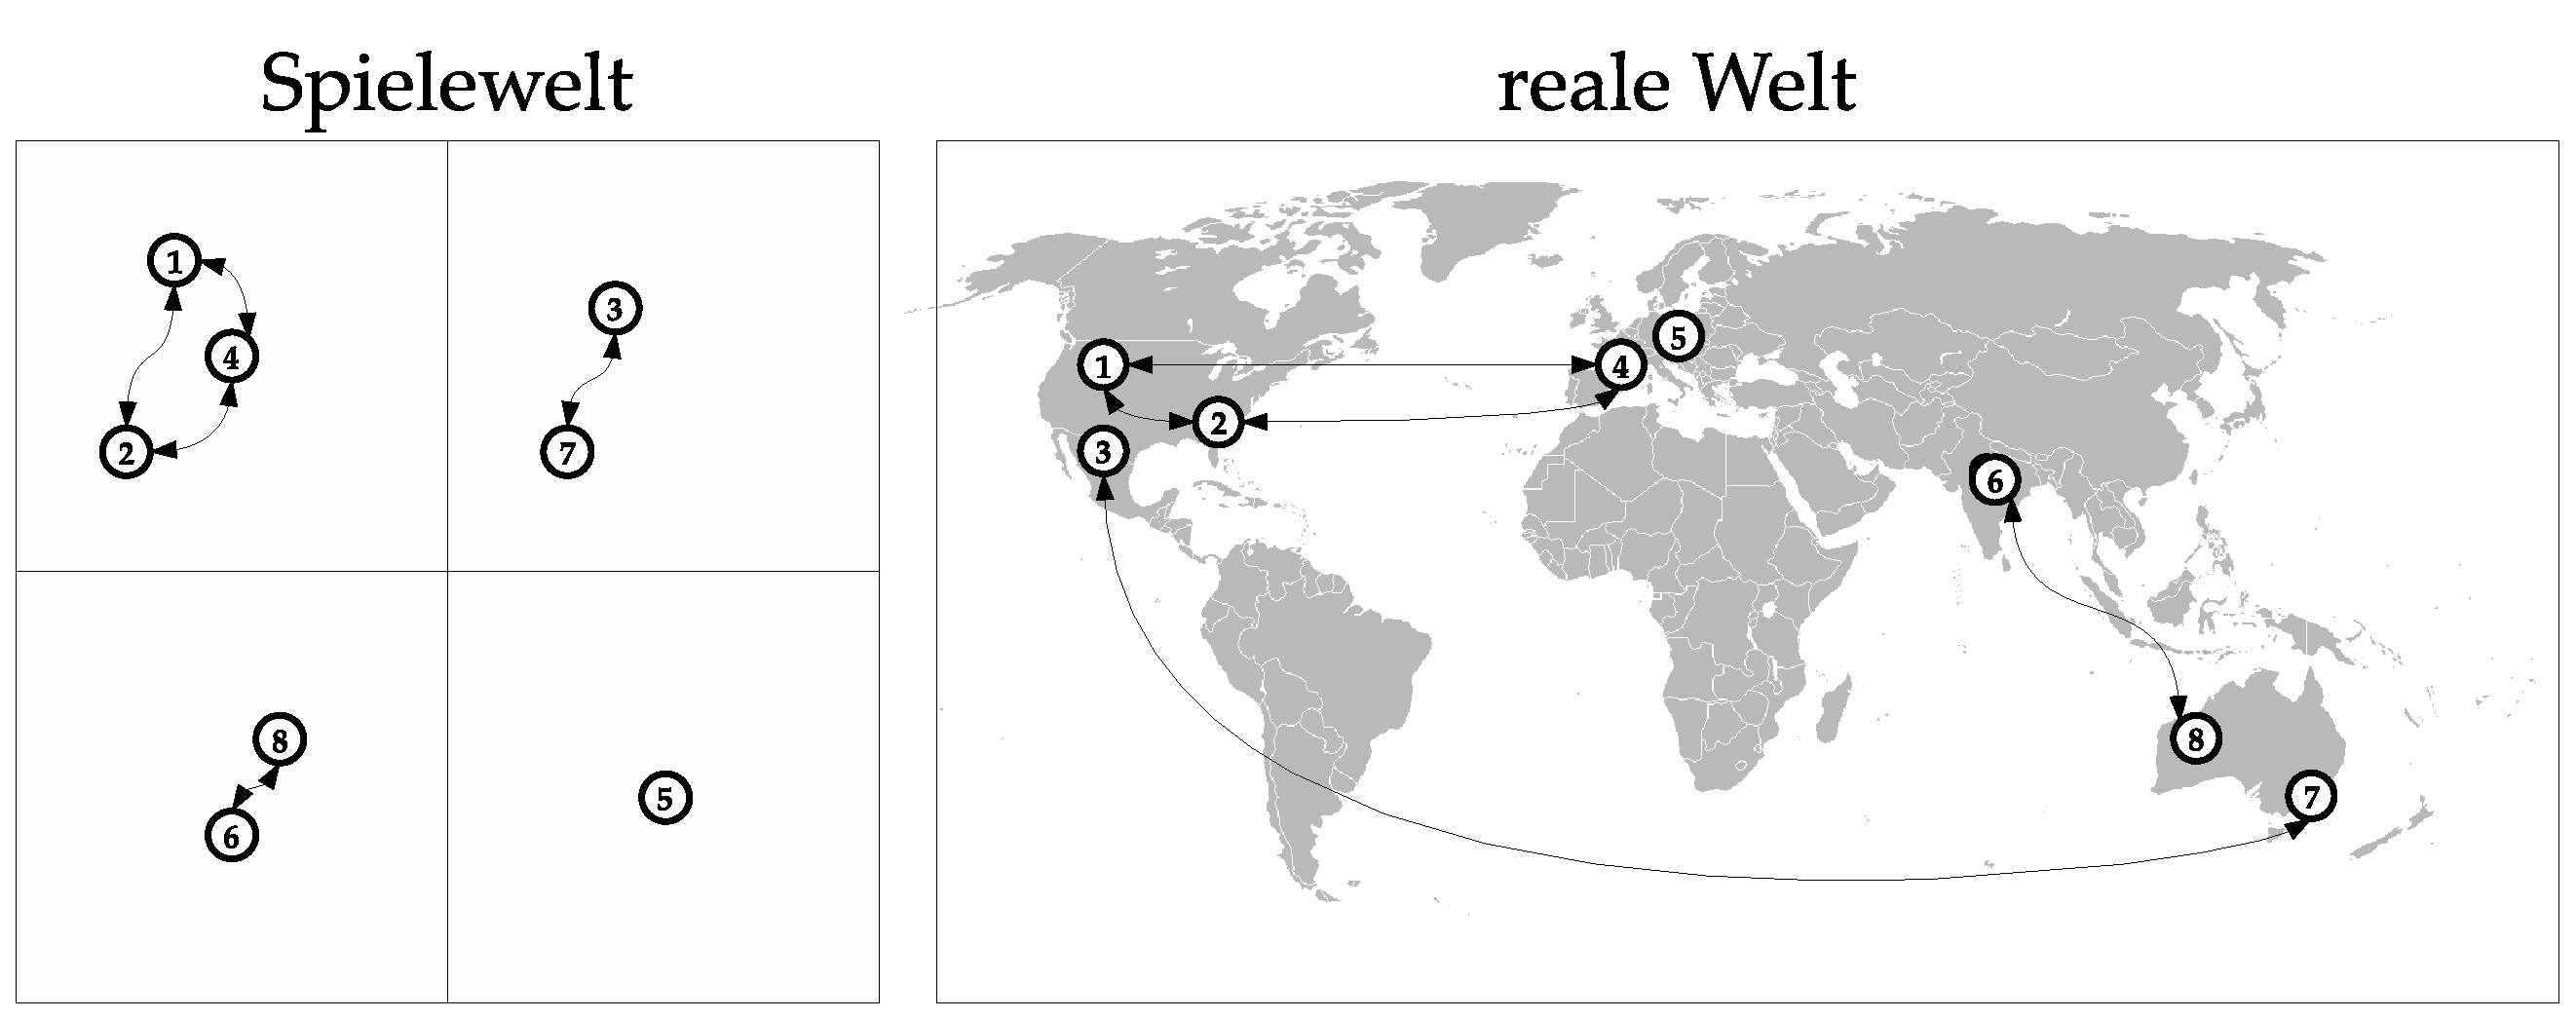
\includegraphics[width=1.00\textwidth]{grafiken/entwurf-p2p.eps}
		\caption{Peer-to-Peer-Architektur mit direkten Audioverbindungen der 
		\mbox{Spieler} untereinander in den entsprechenden Spielezonen}
	\label{fig:entwurf-p2p}
\end{figure}

Der Hauptnachteil dieser Topologie liegt darin, dass die Bandbreite der einzelnen Knoten im Peer-to-Peer-Ansatz die Anzahl der maximal m�glichen Verbindungen limitiert. Im Gegensatz zu Client-Server-Systemen hat die Avatar\-dichte Einfluss auf die Netzwerklast, aber nicht die Gesamtanzahl der Spieler. Obwohl jeder Client nur seinen Teil der Spielewelt verwaltet und nur ben�tigte Audioverbindungen aufbaut, f�hrt die Zunahme der Avatardichte in einer Region zu einem quadratischen Anstieg der Netzwerklast, weil bei einer Konferenz mit N Teilnehmern $N^2-N$ Audiostr�me ausgetauscht werden m�ssen. Dies f�hrt dazu, dass diese Architektur bei einer zu hohen Avatardichte nicht skaliert. 

\subsection{Client-Server}
\label{client-server-verteilung}
In einer Client-Server-L�sung wird der Audiostrom von jedem der Teilnehmer an einen zentralen Audioserver gesendet. Mithilfe der Positionsdaten der Spieler wird die Audioszene dort zentral abgemischt. Diese wird danach an die jeweiligen Spieler gesendet. 

Als Hauptvorteil erweist sich: Jeder Client -- auch mit beschr�nktem Up- und Download -- ist im Stande an solchen Konferenzen teilzunehmen. Auch die Anforderungen an die Rechenkapazit�t bei den Clients sind minimal, da kein lokaler Abmischvorgang stattfinden muss. Das interaktive Delay ist bei einem zentralen Audioserver weder von der Zunahme der Avatardichte noch deren Verteilung oder der Gesamtanzahl der Spieler abh�ngig. 

\begin{figure}[tbh]
	\centering
		\includegraphics[width=1.00\textwidth]{grafiken/entwurf-server.eps}
	\caption{Client-Server-Architektur mit zentralem Mischserver in Nordamerika}
	\label{fig:entwurf-server}
\end{figure}

Ein wichtiger Nachteil besteht darin, dass das interaktive Delay sehr stark von der geografischen Position der zentralen Komponente abh�ngt. So k�nnen f�r die Teilnehmer gro�e Delays auftreten, wenn sie sich physikalisch weit entfernt vom Server befinden. Bei einem falsch positionierten Server kann das Delay f�r einzelne Teilnehmer entsprechend schlecht ausfallen (siehe Abbildung \ref{fig:entwurf-server} Teilnehmer 6,7 und 8).
 M�chte man Clients die Kontrolle �ber alle Audiostr�me �berlassen und findet kein Mischvorgang auf dem Server statt, so ersch�pft sich schnell seine Kapazit�t, da f�r $N$ eingehende Audiostr�me $N^2-N$ ausgehende Str�me verschickt werden m�ssen. 
 
 Auch wenn beim Audioserver ein Mischvorgang stattfindet und f�r N Teilnehmer nur N Audiostr�me ausgetauscht werden m�ssen, ersch�pfen sich ab einer zu gro�en Gesamtspieleranzahl sowohl seine Leistungs- als auch die Bandbreitenkapazit�ten. Da der fundamentale Nachteil dieser Architektur in der seiner fehlenden Skalierbarkeit liegt, werden nachfolgend zwei alternative Systeme vorgestellt, um die Last zu verteilen. 
 
 Spieler der gleichen Umgebung der realen Welt werden an den gleichen Audioserver verwiesen, was dem "`Audio-Proxy-Konzept"' entspricht. Das Konzept der "`verteilten Audioserver"' sieht vor, dass Spieler der gleichen Umgebung der virtuellen Welt dem gleichen Server zugeteilt werden.

\subsubsection{Audio-Proxy}
\label{Audio-Proxy}
Zun�chst muss festgehalten werden: Der Begriff Proxy wird hier anders als in der Literatur �blich verwendet. Als Proxy werden in Rechnernetzen normalerweise Vermittler bezeichnet, die auf der einen Seite Anfragen entgegennehmen, um dann �ber ihre eigene Adresse eine Verbindung zur anderen Seite herzustellen. 

Mit einer Audio-Proxy-L�sung sind dedizierte Mischserver gemeint, die durch ihre weltweite Verteilung eine geringe Entfernung zum Teilnehmer erm�glichen sollen. Diese empfangen die Audiostr�me der Clients, mischen sie ab und schicken sie an die jeweiligen Spieler zur�ck. Proxys k�nnen ebenfalls Audiostr�me an weitere Proxys weiterleiten, falls diese f�r eine Audioszene ben�tigt werden. 

Die Vorteile eines solchen Konzepts liegen darin, dass im Gegensatz zur Peer-to-Peer-Architektur durch den Einsatz von dedizierten Proxys mit guter Anbindung Bandbreitenprobleme minimiert werden. Bei einer Zunahme der Gesamtanzahl der Spieler helfen Proxys auch, die Last des zentralisierten Systems zu verteilen, weil sie Audiostr�me verteilt entgegennehmen und mischen k�nnen. Durch ihre guten Bandbreiten- und Leistungskapazit�ten k�nnen sie jeweils eine hohe Avatardichte und �nderungen der Avatarverteilung gut bew�ltigen. Befinden sich die Teilnehmer einer Audioumgebung alle auch in physikalischer N�he zum Server, d.h. existiert eine starke Korrelation zwischen der realen und virtuellen Welt, erhalten alle Teilnehmer dieser Audioumgebung auch ein niedriges interaktives Delay.  

\begin{figure}[tbh]
	\centering
		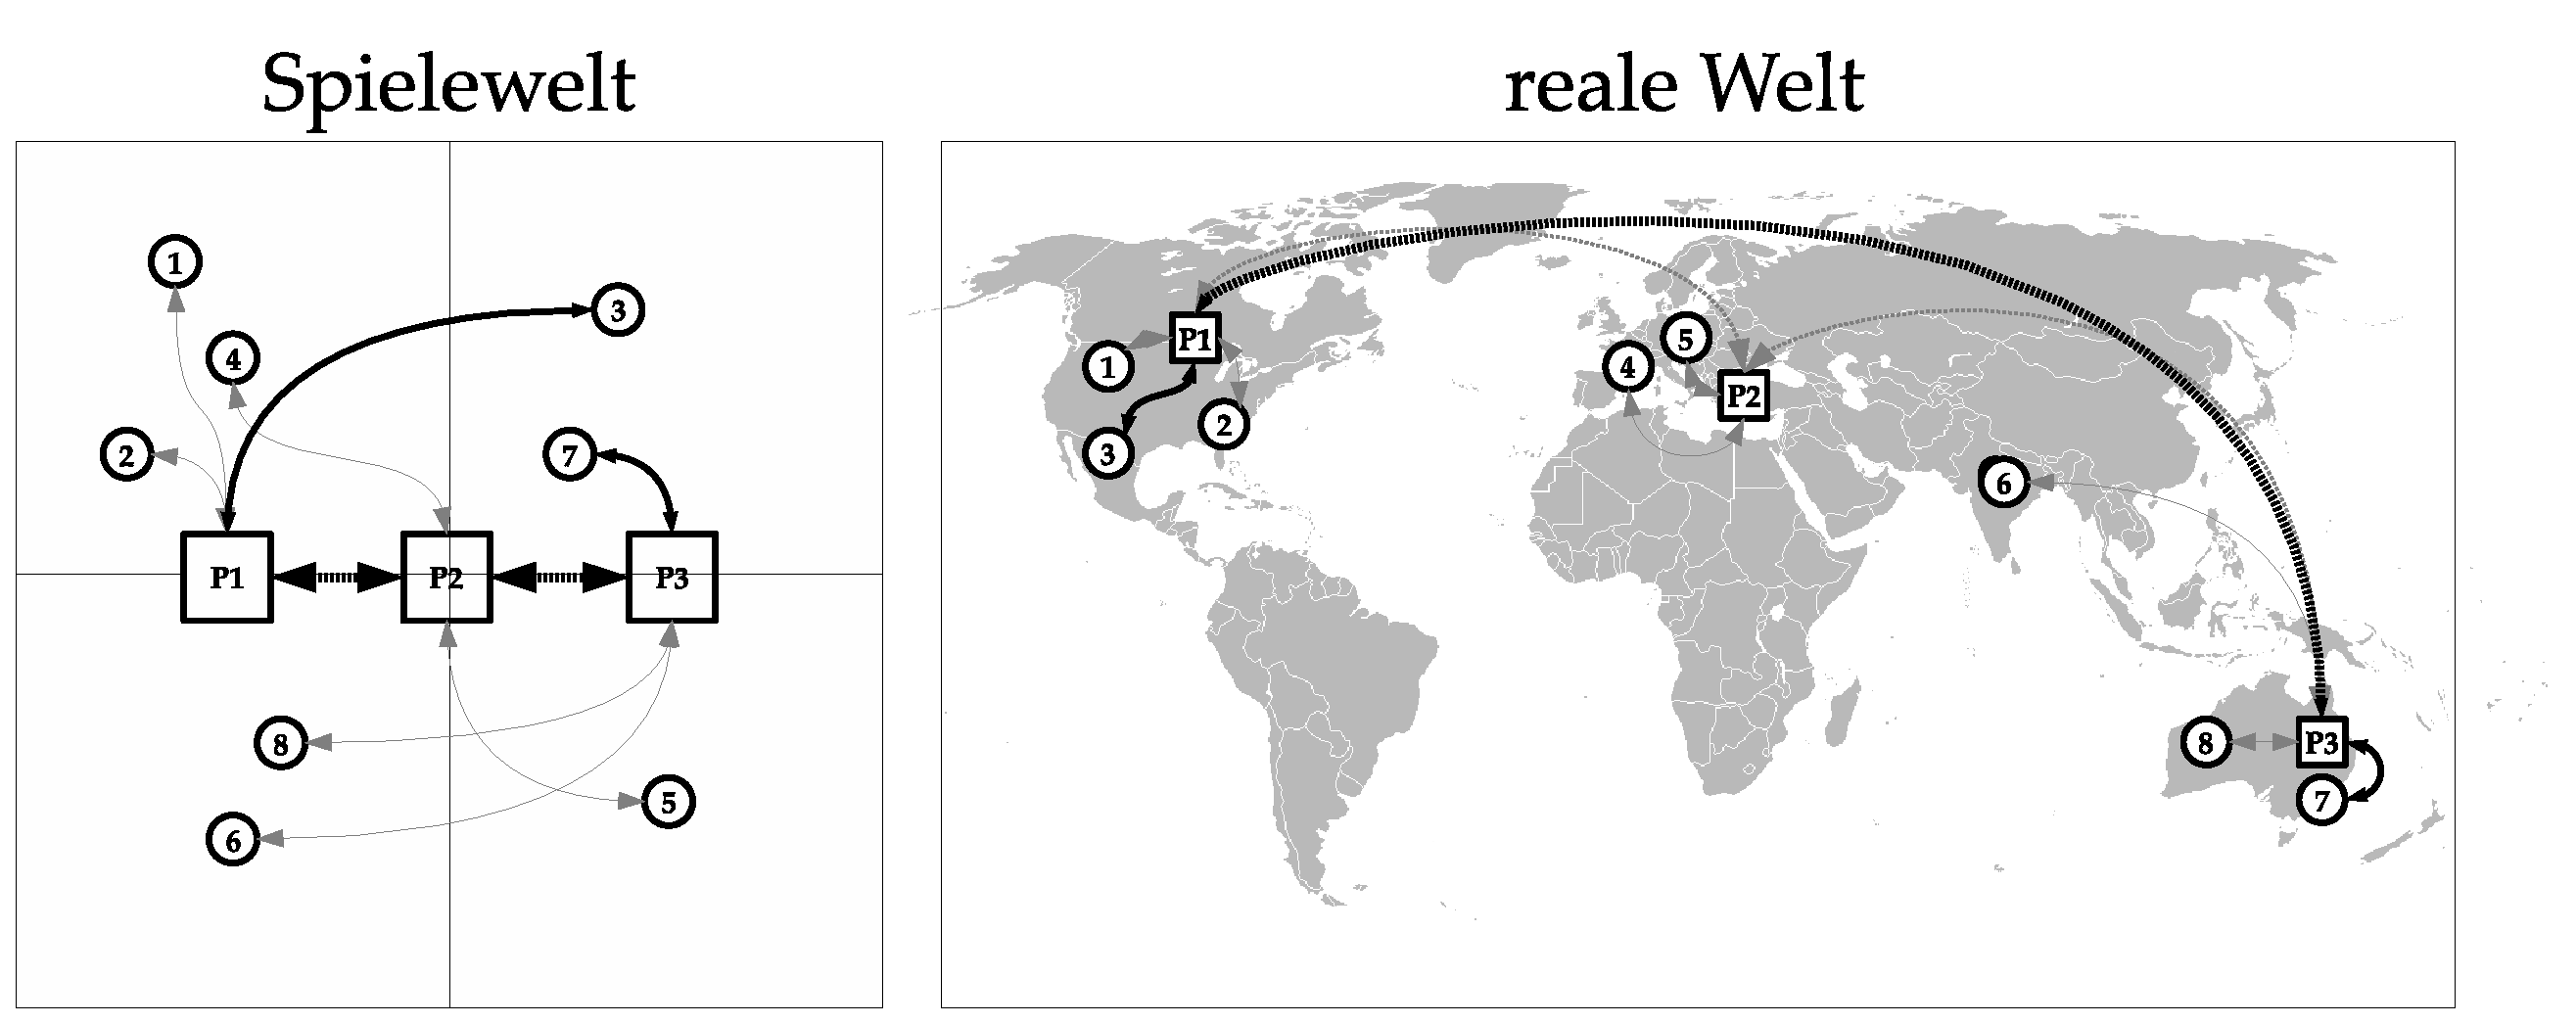
\includegraphics[width=1.00\textwidth]{grafiken/entwurf-proxy.eps}
	\caption{Beispiel f�r eine Proxy-Architektur. In Schwarz ist die Verbindung von Spieler 3 mit Spieler 7 dargestellt.}
	\label{fig:entwurf-proxy}
\end{figure}

Jedoch kann eine starke Korrelation beider Welten nicht erzwungen werden, was auch den Hauptnachteil dieses Systems ausmacht. Man kann durch das Proxy-Konzept zwar erreichen, dass Spieler der gleichen Umgebung in der realen Welt den gleichen Proxy benutzen, kann sie aber nicht in der Bewegung in der virtuellen Welt einschr�nken, da sie sich ja frei bewegen sollen. Umso mehr Teilnehmer sich in der Umgebung des Spielers befinden und so die Avatardichte erh�hen, desto mehr steigt die Wahrscheinlichkeit, dass auch mehrere verschiedene Proxys eingesetzt werden m�ssen, um die Audioszene zu mischen. Dies f�hrt wiederum dazu, mehr Nachrichten m�ssen zwischen den Proxys untereinander weitergeleitet werden, was letztendlich zu einer Verschlechterung des interaktiven Delays f�hrt.

\subsubsection{Verteilte Audioserver}
\label{verteilteaudioserver}
In einer verteilten Server-L�sung ist jeder zentrale Server nur f�r einen Teil der Spielewelt verantwortlich. So nutzen Spieler, die sich in der gleichen virtuellen Umgebung befinden den gleichen Server, der ihre Audiostr�me abmischt. Dieser Ansatz kann die auftretenden Kapazit�tsprobleme einer zentralisierten L�sung reduzieren, indem die Last auf mehrere Server verteilt wird. Die Netzwerklast h�ngt auch hier wie bei allen Serversystemen von der Gesamtspieleranzahl auf dem jeweiligen Server ab. 

Verteilte Audioserver bieten die gleichen Vorteile wie Audio-Proxys, besitzen jedoch auch die gleichen Nachteile. Wie bei den Audio-Proxys gilt auch hier, dieses System funktioniert bei einer starken Korrelation beider Welten gut, diese kann aber nicht erzwungen werden. Man kann zwar durch das verteilte Server-Konzept erreichen, dass Spieler der gleichen Umgebung in der virtuellen Welt den gleichen Server benutzen, hat dann aber keinen Einfluss darauf, wie ihre Verteilung in der realen Welt ist, da man von �berall am Spiel teilnehmen kann. 

�hnlich wie beim Proxy-Konzept hat hier eine Zunahme der Avatardichte einen negativen Einfluss auf das interaktive Delay. Mit einer Zunahme erh�ht sich die Chance, dass Spieler der gleichen Spielregion aus verschiedenen Teilen der Welt stammen k�nnen. Diese Tatsache erh�ht die Wahrscheinlichkeit, dass der entsprechende Server sich nicht im "`Schwerpunkt"' aller Spieler befindet. Somit kann das jeweilige Delay f�r einige Spieler sehr gut ausfallen, f�r andere jedoch sehr schlecht.

\begin{figure}
	\centering
		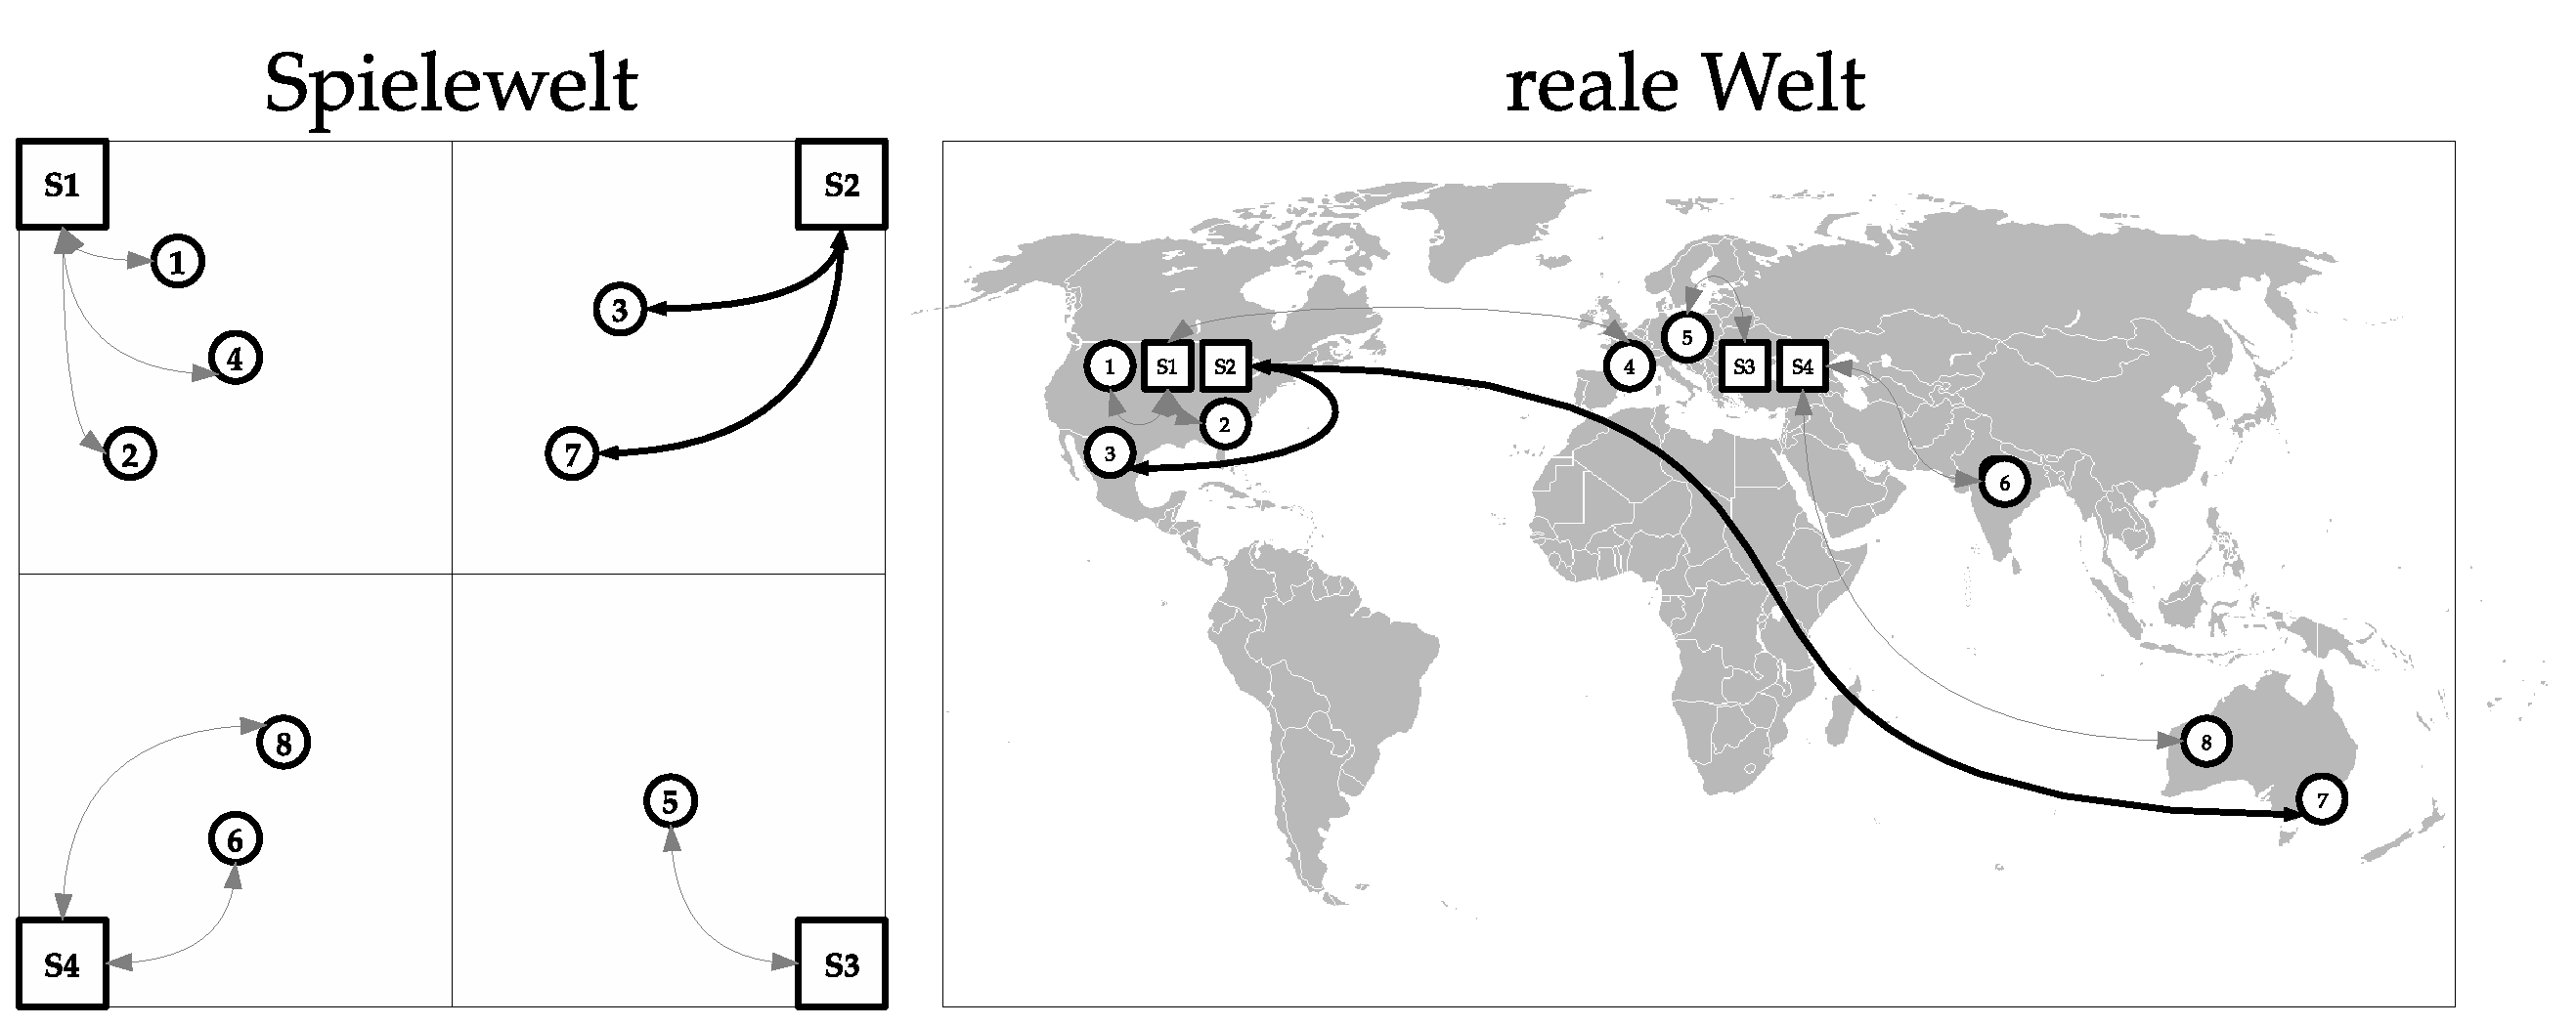
\includegraphics[width=1.00\textwidth]{grafiken/entwurf-verteilteserver.eps}
	\caption{Verteilte Server S1...S4. Die Verbindungen der Spielewelt S2 werden in Schwarz dargestellt. }
	\label{fig:entwurf-verteilteserver}
\end{figure} 

Neue Probleme entstehen beim �bergang von einem Server zum anderen. Wenn Teilnehmer w�hrend des Spiels die Spielzone wechseln und ihre Audiostr�me nun von einem anderen Server abgemischt werden sollen, k�nnen Server abh�ngig von ihrer Lage unterschiedlich hohe Delays liefern und in Grenzbereichen der Spielewelt Probleme auftreten, wenn der Audioserver oft gewechselt wird.

\subsection{Hybrid}
Im Ansatz einer Hybrid-Architektur senden die Teilnehmer ihre Audiostr�me zwar an einen zentralisierten Server, k�nnen sie aber bei Bedarf auch direkt austauschen, wenn die indirekte Route �ber den Server zu hohen Delays f�hren w�rde. Der hybride Ansatz k�nnte zwar alle Vorteile von Peer-to-Peer-Systemen mit zentralisierten Systemen kombinieren, ist allerdings nicht einfach umzusetzen, da nicht klar definiert ist, wann ein Teilnehmer zentral abgemischt werden soll und wann der Audiostrom direkt zwischen den Clients ausgetauscht wird; zudem erfordert er eine hohe Koordination zwischen den Teilnehmern.

\section {Architekturen mit SIP-Komponenten}
Entsprechend der vorgestellten Architekturen gibt es einige M�glichkeiten, Konferenzen mit mehreren Teilnehmern in SIP zu realisieren. 

Prinzipiell m�ssen aber bei einer Umsetzung zwei Fragen beantwortet werden:

\begin{itemize}
	\item Wie und wo findet die Signalisierung der Konferenzen und die Lokation der Teilnehmer statt?
	\item Wie und wo findet das Abmischen des Audiostroms statt?
\end{itemize}

%Auch interessant:
%http://www.ietf.org/internet-drafts/draft-ietf-simple-simple-02.txt

Diese zwei Aspekte k�nnen nicht getrennt voneinander betrachtet werden, da immer die Wahl einer Architektur Einfluss auf beide Probleme hat. In einer Peer-to-Peer-basierten Architektur ist es z. B. zun�chst keine triviale Aufgabe, eine Lokation aller Teilnehmer vorzunehmen, da jeder Peer nur einen Teil der Spielewelt verwaltet und keine zentralisierte Instanz existiert, die �ber alle Positionen aller Spieler verf�gt.  Genauso ergeht es dem zentralisierten System, in dem die Lokation und Signalisierung der Teilnehmer zwar durch eine zentrale Komponente einfach, eine Verteilung des Audiostroms aber problematisch ist. 

So muss f�r Konferenzen nicht nur die Frage beantwortet werden, wo der Audiostrom abgemischt wird, sondern wie die Teilnehmer informiert werden, dass sie Teil einer Konferenz sind.

Zus�tzlich zu diesen Fragen muss eine gew�hlte Architektur in Bezug auf die Herausforderungen aus Kapitel 3 noch folgende Kriterien erf�llen:

\begin{itemize}
	\item Die Architektur muss mehrere Audiostr�me unterst�tzen.
	\item Jeder Client muss in der Lage sein, alle Audiostr�me lokal zu kontrollieren.
\end{itemize}

%Deswegen werden die Komponenten zur Lokation, Signalisierung der Konferenzen und Mischen des Audiostroms zwar gleichzeitig betrachtet, aber unter ihnen unterschieden.

\subsection{Komponenten}
\label{sipkomponenten}
Es k�nnen drei Hauptkomponenten eines Systems definiert werden, die je nach ihrer Verteilung verschiedene Architekturen bilden k�nnen:

\begin{itemize}
	\item \textbf{Mixer}: Ein Mixer empf�ngt eine Gruppe von Audiostr�men und vereinigt ihre Medien nach einer spezifischen Art, um das Ergebnis an jeden Teilnehmer zu schicken. Dies beinhaltet Medien, die mittels des RTP-Protokolls �bertragen wurden.
	\item \textbf{Konferenz-Komponente:} Eine Konferenz-Komponente ist die logische Instanz, die dar�ber entscheidet, welche Audiostr�me miteinander gemischt werden, an wen sie verteilt werden und auch wer Teilnehmer einer Konferenz ist. Die Konferenz-Komponente kann von der Spielelogik gesteuert werden. Im SIP-Standard beinhaltet diese Komponente einen Proxy und/oder Registrar. 
	\item \textbf{Teilnehmer-Client}: Eine Client-Anwendung verbindet einen Benutzer mit einer Konferenz. Diese implementiert mindestens einen SIP-User-Agent kann aber auch nicht SIP-spezifische Mechanismen f�r zus�tzliche Funktionalit�t beherbergen. 
	%\item \textbf{Spieleserver}: Eine optionale Komponente, die die Daten der Spieler entgegen nimmt, um sie auszuwerten und an die anderen Teilnehmer zu verteilen. Diese kann, muss aber nicht, die Spielelogik enthalten und teilt dem Konferenz-Server mit, welche Spieler Teil einer Konferenz werden. Um mit den anderen Komponenten zu kommunizieren unterst�tzt sie das SIP Protokoll. 
\end{itemize}

%\subsection{Einsatz mehrerer Server}
%\label{mehrereregistrare}

Aus den vorgestellten Komponenten wird ersichtlich: Die Architektur der Sprachkommunikation kann nicht getrennt von der Architektur der darunter liegenden Signalisierung gesehen werden. Dies geschieht, da die Signalisierung und der reine Austausch an Spielerinformationen und Konferenzinformationen relativ wenig Bandbreite ben�tigt. Eine Audioverbindung dagegen kann aufgrund ihres reinen Datenvolumens bereits das Zehnfache der Bandbreite ben�tigen.   

Geht man davon aus, dass sowohl die Signalisierung als auch die Audiostr�me zwischen den Spielern entweder komplett zentral verteilt oder komplett dezentral stattfinden k�nnen, ergeben sich 9 m�gliche Kombinationen, die in Tabelle \ref{audiodatenmatrix} dargestellt werden. Bei einem zentralen System wird genau ein Server eingesetzt, bei einem dedizierten System werden mehrere Server oder besonders leistungsf�hige Clients eingesetzt, bei einem P2P-System existieren keine Server. Dabei kann beim dedizierten Verteilen von Audioservern jede Technik aus Abschnitt \ref{client-server-verteilung} eingesetzt werden. 

\begin{flushleft} 
\begin{table}[tbh]
	\centering	\begin{tabular}{p{0.15\textwidth}|p{0.24\textwidth}|p{0.24\textwidth}|p{0.24\textwidth}}
		\toprule
		\textbf{Daten / \newline Audio} & \textbf{Zentral} & \textbf{Dediziert} & \textbf{P2P} \\
		\midrule
		\textbf{Zentral} & ($A_{1}$) Client-Server Paradigma & ($A_{4}$) Ein Audioserver und mehrere Datenserver & ($A_{7}$) Ein Audioserver, aber dezentrale Signalisierung\\
		\hline
		\textbf{Dediziert} & ($A_{2}$) Zentraler Server mit mehreren dedizierten Audioservern & ($A_{5}$) dedizierte Daten- und Audioserver oder Supernodes& ($A_{8}$) Dedizierte Audiomixer, dezentrale Signalisierung\\
		\hline
		\textbf{P2P} & ($A_{3}$) VoIP mit zentralem Server & ($A_{6}$) VoIP mit mehreren Servern & ($A_{9}$) Komplett dezentrale L�sungen. \\
		\bottomrule
		\end{tabular}
	\caption{M�gliche Kombinationen bei Unterscheidung zwischen Daten- und \mbox{Audiostr�men}}
\label{audiodatenmatrix}
\end{table}
\end{flushleft} 

Prinzipiell sind alle Alternativen vorstellbar. In erster Linie sollen bei einer Implementierung einer einsatzf�higen Sprachkommunikationsl�sung vor allem Alternativen bevorzugt werden, die sowohl umsetzbar sind und sinnvoll erscheinen als auch eine Umsetzung der Vorschl�ge aus Kapitel 3 erf�llen k�nnen.  

\begin{itemize}
	\item ($A_{1}$) Hier findet sowohl die Signalisierung und Lokation der Teilnehmer als auch das Mischen des Audiostroms zentral statt. Darunter versteht man ein SIP-Netzwerk, das mit einem zentralen Server ausgestattet ist, der s�mtliche Daten der Spielerclients entgegennimmt und alle Konferenzen koordiniert. Das Abmischen der Audiostr�me findet ebenfalls in einer oder mehreren zentralen Konferenzen statt, die auf dem Server verwaltet werden. 	
	\item ($A_{2}$) Beh�lt man eine zentrale Konferenzkomponente bei, geht aber von einem verteilten Abmischen der Audiostr�me aus, kann man entweder mehrere dedizierte Mixer einsetzen oder auch einzelne Clients mit gen�gend Bandbreite (Superpeers) nutzen, um den Audiostrom zu mischen und dann zu verteilen (siehe Abschnitt \ref{verteilteaudioserver} und \ref{Audio-Proxy}).
	\item ($A_{3}$) Im hybriden Modell besitzt das System einen zentralen Proxy und Registrar, der die Signalisierung und Lokation der Teilnehmer vornimmt; das Abmischen der Audiostr�me findet dagegen dezentral und lokal bei jedem Client statt. Dies entspricht dem urspr�nglichen SIP-Aufbau, bei dem die Sprachkommunikation zwischen den einzelnen Peers stattfindet und das Audiosignal lokal von jedem Teilnehmer abgemischt wird.
	\item ($A_{4}$) Setzt man mehrere Proxys oder verteilte Server f�r den Datenaustausch ein, mischt aber die Audiostr�me zentral ab, so wird genau ein dedizierter Mixer eingesetzt, der alle Audiostr�me entgegennimmt und abmischt, w�hrend die Sig\-nali\-sierung �ber mehrere Proxys verteilt wird. 
	\item ($A_{5}$): Realisiert man sowohl den Datenaustausch als auch das Mischen des Audiostroms verteilt, geht man davon aus, dass entweder dedizierte Audio- und Datenkomponenten zusammenarbeiten oder auch besonders gut angebundene Clients (Superpeers) die Signalisierung und das Mischen des Audiostroms vornehmen.
	\item ($A_{6}$): Die Signalisierung und Lokation werden von mehreren verteilten Proxys oder Registraren �bernommen, w�hrend die Clients f�r das Abmischen ihrer Audiostr�me verantwortlich sind.
	\item ($A_{7}$): W�hrend ein dedizierter Audioserver das Abmischen der Audio\-str�me vornimmt, findet der Datenaustausch komplett dezentral statt. 
	\item ($A_{8}$): Auch hier findet ein komplett dezentraler Datenaustausch statt, w�hrend nun mehrere dedizierte Audioserver sich das Abmischen der Audiostr�me aufteilen. 
	\item ($A_{9}$): Realisiert man sowohl den Datenaustausch als auch das Mischen des Audiostroms komplett dezentral, 	spricht man vom Einsatz eines dezentralisierten SIP-Netzwerkes, das mittels P2P SIP, Multicast oder Full-Mesh-Ans�tzen realisiert werden kann. 
\end{itemize}

Die vorgestellten Alternativen $A_{4}$, $A_{5}$ und $A_{6}$ gehen davon aus, dass die zentrale Komponente des Registrars auf mehrere Server verteilbar ist. Von einer Verteilung des Registrars und des Proxy k�nnen auch die vorgestellten Alternativen $A_{1}$, $A_{2}$, $A_{3}$ profitieren, da sich damit die \textit{Fehlertoleranz} des Systems erh�ht. Falls mehrere Registrare eingesetzt werden, bestehen folgende Alternativen\footnote{Die Nachteile dieser Ans�tze bei einer gro�en Benutzeranzahl sind entweder eine gro�e Netzwerklast oder eine hohe Verbindungslatenz.}:
\begin{itemize}
	\item Die Registrierung des Benutzers findet auf einem Registrar statt und wird dann mit Datenbank-Replikation konsistent auf mehrere Registrare repliziert. Die Suche findet bei einem beliebigen Registrar statt.  
	\item Die Registrierung geschieht nur auf einem Registrar, w�hrend die Suche nach dem Registrar, der die Benutzerinformation enth�lt vom Client auf allen Registraren stattfindet. Dazu muss der Benutzer alle Registrare kontaktieren oder der erste kontaktierte Server die Anfrage weiterleiten. 
\end{itemize}

%Der Nachteil des ersten Ansatzes ist eine erforderliche Synchronisation f�r jede Registrierung. Es besteht die M�glichkeit, dass Eintr�ge veraltet sind, bevor eine Synchronisation zwischen den Servern ausgef�hrt wird. Mit einer wachsenden Anzahl an Benutzern k�nnte der zus�tzliche Netzwerkverkehr zwischen den Servern zu einem Flaschenhals werden. 
%Im anderen Fall ist die Verbindungslatenz h�her, da erst eine Reihe von Schritten durchlaufen werden muss. Eine parallele Suche erh�ht zudem die ben�tigte Bandbreite. 
%Beide Ans�tze k�nnen jedoch fehlschlagen, wenn die Anzahl an Benutzern sehr gro� wird.

Geht man dazu �ber, den Datenaustausch des Spiels komplett dezentral zu organisieren (siehe Alternativen $A_{7}$,$A_{8}$,$A_{9}$), so geschieht das aus zwei Gr�nden: erstens, um einen Single Point of Failure zu vermeiden und zweitens, um eine bessere Skalierbarkeit zu erreichen. 

Prinzipiell ist dieses Vorgehen solange praktikabel, wie noch einige zentrale Komponenten bestehen, die hierarchisch h�her gestellt sind als andere Knoten. Dies ist schon aus Gr�nden wie z. B. der Konferenzsteuerung notwendig, da Knoten existieren m�ssen, die die Lokationen der einzelnen Teilnehmer kennen, Rechte in Konferenzen �berwachen, oder eine Liste an aktiven Teilnehmern f�hren.

 Ans�tze zu einer komplett dezentralen Signalisierung werden sp�ter im Kapitel 8 vorgestellt, es darf aber schon vorab festgehalten werden, dass ein hoher Aufwand betrieben werden muss, um skalierbare dezentrale Systeme zu konstruieren. Nimmt man  diesen Aufwand tats�chlich auf sich, so erscheint es unlogisch, noch zentrale Audioserver-Komponenten zu behalten, da man so wieder einen Single Point of Failure besitzt und diese nicht skalieren. Das f�hrt zur logischen Entscheidung, alle Kombinationen, welche eine dezentrale Signalisierung besitzen, die aber trotzdem dedizierte Audioserver einsetzen, nicht weiter zu analysieren. Davon sind die Alternativen ($A_{7}$) und ($A_{8}$) betroffen.

Genauso verh�lt es sich bei der Skalierbarkeit: Der Grund, mehrere Server einzusetzen, liegt -- wie bereits erw�hnt -- darin, die ansteigende Netzwerklast zu verteilen. Beh�lt man jedoch einen einzigen zentralen Audioserver bei, so bildet dieser schnell den Flaschenhals. Deswegen wird die Alternative ($A_{4}$), die verteilte Spieleserver, aber einen zentralen Audioserver einsetzt, vorerst nicht weiter untersucht.

Die verbleibenden Alternativen lassen sich in 4 Gruppen gliedern:
\begin{itemize}
	\item Komplett zentralisierte Ans�tze (Alternative $A_{1}$)
	\item Komplett dezentralisierte Ans�tze (Alternative $A_{9}$)
	\item Ans�tze, die verteiltes dediziertes Audiomixing vornehmen (Alternativen $A_{2}$ und $A_{5}$)
	\item Ans�tze, die komplett dezentrales Audiomixing vornehmen (Alternativen $A_{3}$ und $A_{6}$)
\end{itemize}

\subsection{Komplett zentralisierte Ans�tze}
\label{zentralansatz}

\begin{figure}[tbh]
	\centering
		\includegraphics[width=0.8\textwidth]{grafiken/archzentral.eps}
	\caption{Komplett zentralisierter Ansatz mit SIP}
	\label{fig:archzentral}
\end{figure}

Beim Einsatz der Alternative $A_{9}$ wird die Signalisierung und Lokation der Teilnehmer und das Abmischen der Audiostr�me zentral vorgenommen. Die in Kapitel 5 von Singh und Acharya vorgestellte Methode kann man als zentralisiertes SIP-System bezeichnen. Den komplett zentralisierten Ansatz verfolgen auch Safei und Boustead im vorgestellten MICE-System. Diese Architektur bietet zun�chst eine sehr gute Ausgangsbasis f�r Sprachkommunikationsl�sungen mit einer begrenzten Anzahl an Teilnehmern, da es auch Knoten mit geringer Bandbreite eine Teilnahme erm�glicht. 

Die Grundlage f�r eine einfache Berechnung der maximal m�glichen Anzahl an Spielern auf einem Server versteht sich unter folgenden Voraussetzungen:

\begin{itemize}
	\item Jeder Spieler sendet einen Audiostrom zum Server.
	\item Jeder Spieler im gleichen Spiel m�chte die gesprochenen Daten aller Spieler empfangen.
	\item Weil der Spiele-/Konferenzserver und Mixer zentralisiert sind, kann der Mixer die Audiostr�me zentral abmischen, da er auch die Positionen der Teilnehmer kennt. 
\end{itemize}

Befinden sich beispielsweise 16 Personen im Spiel, empf�ngt der Server Audio\-str�me von 16 Personen und sendet einen bereits abgemischten Audiostrom an jede der 16 Personen. 

Sendet jeder Spieler seinen Audiostrom mit einem Speex-Audiocodec\footnote{Patentfreies Audio-Kompressions-Format (Xiph OSC), Seite besucht 22.03.2008, http://speex.org} mit einer 16 Kbit/s Bitrate an den Server, der nach dem heutigen Standard mit einer 100MBit-Anbindung f�r den Up- und Download ausgestattet ist, w�rde sich folgende theoretische maximale Anzahl an gleichzeitigen Audioverbindungen ergeben:

\[
 \frac{100000 \frac{Kbit}{s}}{16 \frac{Kbit}{s}} = 6250 \, Spieler
\]

Der Client selbst dagegen muss nur in der Lage sein, seinen eigenen Audiostrom zu senden und einen Audiostrom mit gleicher Bitrate zu empfangen. 

Obwohl diese Rechnung zun�chst vielversprechend klingt, muss auch die Rechenkapazit�t des Servers ber�cksichtigt werden, da jedes der ankommenden Signale dekodiert, abgemischt und kodiert werden muss. Eine Messung\footnote{Siehe Kapitel 9: Evaluation} der CPU-Belastung des Mixers, die anhand der Implementierung vorgenommen wurde, zeigt, dass die praktisch maximal m�gliche Anzahl an Spielern schon mitunter bei 32 Spielern erreicht wird, wenn ein rechenintensives Resampling des Audiosignals stattfindet. Diese Beobachtung wird auch dadurch best�tigt, dass bisherige Drittanbieter Sprachkonferenzl�sungen f�r Mehrspieler-Computerspiele im Schnitt nur 30-50 gleichzeitige Teilnehmer unterst�tzen\footnote{Ventrilo Server Status Query (Christian Wellh�fer), Seite besucht 23.03.2008, http://ventrilo-monitor.com/}.

Prinzipiell ist dieser Ansatz allen dezentralisierten Ans�tzen �berlegen, da ein zentraler Mischserver in der Regel �ber gen�gend Bandbreite verf�gt, um viele Audiostr�me zu empfangen und zu versenden, w�hrend dies bei Clients oft zu Problemen f�hrt. Zudem besteht die M�glichkeit, die Lokation und Signalisierung der Teilnehmer zentral zu verwalten. Diese Architektur wird vor allem bei Telefonkonferenzen verwendet, bei denen die Endger�te (VoIP-Telefone) �ber eine geringe Rechenleistung verf�gen und auf das Abmischen des Audiosignals durch einen Mischserver angewiesen sind. 

Da jedoch die Bandbreite und Rechnerkapazit�t eines zentralen Audioservers begrenzt sind, �berwiegen die Nachteile, die durch Schwierigkeiten bei der Skalierbarkeit eines zentralen Mischservers entstehen. Erschwerend hinzu kommt das bereits in Abschnitt \ref{client-server-verteilung} beschriebene Problem des interaktiven Delays, das stark von der Position des Servers abh�ngt und entsprechend schlecht ausfallen kann. Da in Kapitel 3 auch gefordert wurde, dass jeder Spieler Kontrolle �ber alle seine Audiostr�me erhalten soll, gestaltet sich au�erdem die Verwaltung und das Abmischen einer jeweils pers�nlichen Konferenz f�r jeden Spieler sehr schwer. Zuletzt sind noch die hohen Kosten beim Einsatz eines zentralen dedizierten Servers zu bedenken. All diese Gr�nde sprechen gegen den Einsatz einer solchen Architektur. 

Dabei bietet es sich gerade im Spielebereich an, die hohe Rechenleistung von gut ausgestatteten Spielecomputern auszunutzen, um die zentrale Komponente zu entlasten. 

\subsection{Komplett dezentralisierte Ans�tze}

\begin{figure}[tbh]
	\centering
		\includegraphics[width=0.80\textwidth]{grafiken/archp2p.eps}
	 \caption{Dezentralisierte SIP-Architektur}
	\label{fig:archp2p}
\end{figure}

Ans�tze der Alternative $A_{9}$ haben alle gemeinsam, dass sowohl der Audiostrom als auch der Datenstrom nur zwischen den einzelnen Knoten flie�t und keine zentrale Komponente ben�tigt wird. Sie unterscheiden sich jedoch darin, in welchen Topologien die einzelnen Clients miteinander verbunden werden und auf welche Art und Weise die Signalisierung stattfindet. Alle komplett dezentralisierten Ans�tze sind sehr gute Kandidaten, um die Anforderungen aus Kapitel 3 zu erf�llen, weil hier jeder Client mit allen Audiostr�men versorgt wird. Der Nachteil solcher Architekturen liegt jedoch in der schwierigen Signalisierung der Teilnehmer, da sich diese in einem komplett verteilten System schwierig gestaltet. 

\subsubsection{Multicast}
Gro� angelegte Multicast-Konferenzen waren die urspr�ngliche Motivation f�r die Entwicklung von SIP. In solchen Konferenzen werden eine oder mehrere Multicast-Konferenzen zu einer Konferenz vereint. Jeder Teilnehmer tritt einer Multicast-Gruppe bei und sendet seine Daten an diese Gruppe. 

Multicast-Konferenzen haben den Vorteil, dass sie keine Koordination zwischen den Endsystemen ben�tigen. Konferenzteilnehmer k�nnen unabh�ngig einer Konferenz beitreten und sie verlassen. 

Der Hauptnachteil von Multicast ist jedoch, dass es nur in einem Local Area Network funktioniert und im Internet nicht allgemein verf�gbar ist. Zudem m�ssen bei solchen Konferenzen Router die Identit�ten der Gruppe speichern und es ist beliebigen Teilnehmern m�glich, solchen Gruppen ohne Authentifizierung beizutreten. 

So verlieren die Teilnehmer die Kontrolle dar�ber, wer an Konferenzen teilnehmen kann und sind auch nicht in der Lage zu wissen, wer ihnen gerade zuh�rt. Abonniert beispielsweise ein falsch konfiguriertes System alle existierenden Multicast-Gruppen, entsteht dadurch ein sehr hoher Bandbreitenverbrauch, der schnell das ganze Netz  fluten kann. Gerade wegen dieser Probleme wird Multicast in wenigen Internet-Hauptleitungen unterst�tzt. Multicast-Konferenzen k�nnen zwar in LANs n�tzlich sein, im kommerziellen Internet sind sie jedoch nicht umsetzbar.

% In the loosely coupled model, there is no signaling relationship between participants in the conference.  There is no central point of control or conference server.  Participation is gradually learned through control information that is passed as partof the conference (using the Real Time Control Protocol (RTCP) [2], for example).  Loosely coupled conferences are easily supported in SIP by using multicast addresses within its session descriptions. 

\subsubsection{Peer-to-Peer-Unicast}
\label{peer-to-peer-unicast}
Bei einem v�llig dezentralisierten P2P-SIP mittels verteilter \textit{Hashtabellen}\footnote{Es existieren mehrere Umsetzungen verteilter Hashtabellen wie CAN \cite{Ratnasamy01}, Chord \cite{Stoica01}, Pastry \cite{Rowstron01} und Tapestry \cite{zaho01}, die sich durch spezielle Eigenschaften voneinander unterscheiden, deren Erl�uterung jedoch �ber den Fokus der Arbeit hinausgeht.} findet sowohl die Lokation, Signalisierung als auch die Sprachkommunikation nur zwischen den einzelnen Clients statt. Bisher existieren zwei Entw�rfe von P2P-SIP-Umzusetzungen \cite{pundkar07},\cite{bryan05s}. Beide Varianten haben gemeinsam, dass die einzige zentrale Komponente des Systems -- der Registrar -- entfernt wird und dezentral zwischen den einzelnen Teilnehmern verteilt realisiert wird, wobei jeder Rechner einen Teil der Funktionalit�t �bernimmt. 

F�r jede Audioverbindung wird ein Peer-to-Peer-Unicast eingesetzt, dessen Vor- und Nachteile in Abschnitt \ref{siphybrid} besprochen werden.

Dieser interessante Ansatz ist bisher nur theoretisch m�glich, da keine geeignete SIP-Implementierung existiert, die einen verteilten Registrar umsetzt. Zudem ist das Problem einer verteilten Spielkontrolle nicht trivial, da kein Teilnehmer �ber komplette Informationen der Spielewelt verf�gt. Sollte in Zukunft eine Implementierung eines funktionierenden P2P-SIP-Overlays existieren, k�nnte diese Option durchaus vorstellbar sein. 

\subsubsection{Full-Mesh}
In einem "`Full-Mesh-Modell"' kommuniziert jeder Endpunkt direkt mit jedem anderen Endpunkt. Alle Teilnehmer in der Konferenz sind "`gleich"', d. h., es gibt keinen Benutzer, der topologisch besonders ist oder �ber zus�tzliche Rechte oder F�higkeiten verf�gt. Jeder Teilnehmer kann jederzeit eine Konferenz betreten und verlassen. Das Audiosignal wird nur von den Endpunkten abgemischt.

Der Hauptvorteil liegt darin, dass ein solcher Aufbau keinen Single Point of Failure besitzt, da alle Komponenten gleichgestellt sind. Bei einem Austausch der Audiostr�me muss jeder Teilnehmer nur seinen eigenen Audiostrom kodieren, und alle N-1 ankommenden Audiostr�me einer N-Teilnehmer Konferenz dekodieren. F�r die meisten Sprachcodecs verursacht das Dekodieren weniger Last als das Kodieren, was also diesem Vorgehen entgegenkommt. 

In einer N-Teilnehmer Konferenz muss jedoch jeder Teilnehmer �ber gen�gend Bandbreite verf�gen, um N-1 simultane Audiostr�me zu verschicken und zu empfangen. Dadurch ist dieser Mechanismus f�r Systeme mit limitierten Bandbreiten wie analoge Modems oder asymmetrische DSL-Leitungen, die vor allem �ber eine schwache Uploadbandbreite verf�gen, nicht besonders gut anwendbar.

Das gr��te Problem bei diesem Ansatz stellt jedoch die fehlende strukturierte Signalisierung und Lokalisierung der Teilnehmer dar, da kein Knoten eine vollst�ndige Information dar�ber besitzt, wer Teil einer Konferenz sein soll. Der in Kapitel 5 vorgestellte Full-Mesh-Ansatz von Schulzrinne enth�lt genau diese Problematik.


\subsection{Verteiltes dediziertes Audiomixing}
\begin{figure}
	\centering
		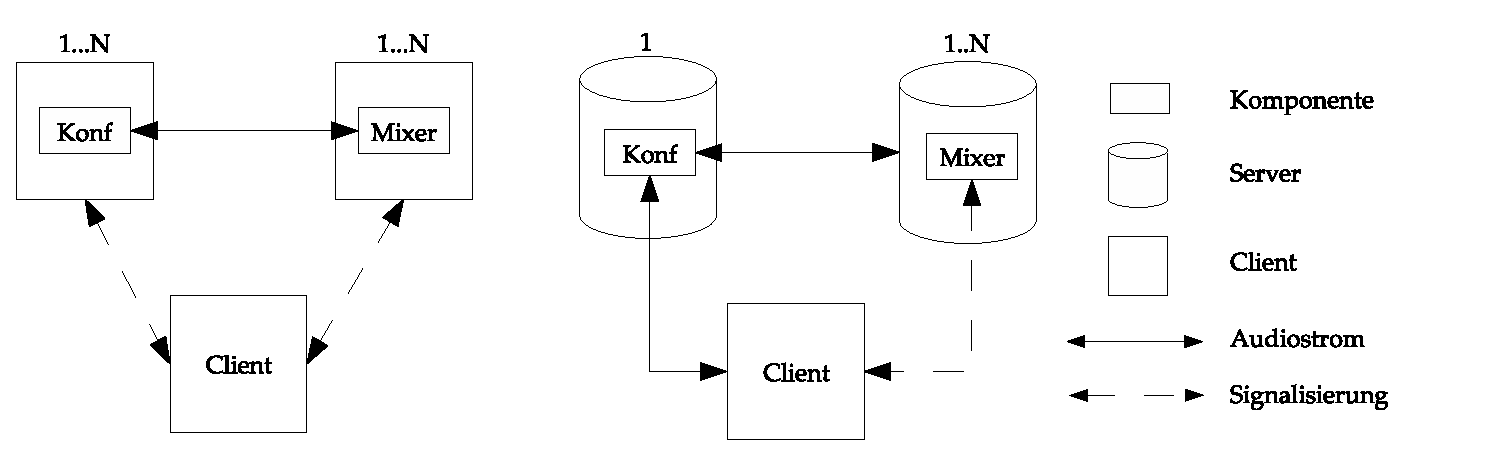
\includegraphics[width=1\textwidth]{grafiken/archverteilt.eps}
	\caption{Architekturen mit mehreren dedizierten Audiomixern}
	\label{fig:archverteilt}
\end{figure}

	Ein Ansatz, verteilte Konferenzen zu betreiben, besteht darin, mehrere dedizierte SIP-Endpunkte zu ernennen, mit denen sich Teilnehmer verbinden. Diese Mixer nehmen die Audiostr�me entgegen, mischen sie ab und leiten sie an die entsprechenden Spieler weiter. Die Signalisierung dagegen kann entweder von einem oder mehreren Registraren vorgenommen werden. 

Dabei gibt es zwei m�gliche Varianten dieses Modells: In einem Superpeer-Mixing �bernimmt ein Client die Verantwortung f�r das Mischen des Audiostroms und in einem Server-basierten-Mixing �bernehmen unabh�ngige dedizierte Server-Knoten diese Verantwortung, ohne aktiv am Gespr�ch teilzunehmen. 

Die Vorteile liegen vor allem in der Verteilung der Bandbreiten- und Kapazit�tsbelastung des Mischvorgangs auf mehrere Maschinen, w�hrend die Signalisierung noch zentral verwaltet werden kann. 

Dieses Modell hat jedoch einige Nachteile: Vor allem beim Einsatz von Super\-peer-Mixing ist die Existenz einer Konferenz ab\-h�n\-gig von dem Vorhandensein des entsprechenden Knotens; geht dieser offline, kann das Abmischen nicht mehr stattfinden. Was die maximale Anzahl an Spielern angeht, ergeben sich hier prinzipiell f�r jeden Mischknoten die gleichen Berechnungen wie bei einem zentralen Server-System (siehe Abschnitt \ref{zentralansatz}). Es erscheint unwahrscheinlich, dass private Rechner heutzutage �ber gen�gend Bandbreite und Rechenkapazit�t verf�gen, um f�r eine signifikante Anzahl an Spielern das Mischen vorzunehmen. Setzt man ein Server-basiertes-Mixing ein, so sind entsprechend hohe Kosten bei dessen Betrieb zu tragen. Da dedizierte Mischserver meist zuverl�ssiger sind und �ber eine bessere Anbindung verf�gen, sind sie besser als Superpeers f�r dieses Verfahren geeignet.

Ebenfalls problematisch gestaltet sich das Auffinden von Superpeer-Mixern, da zuerst alle Teilnehmer den gleichen Knoten aufsuchen m�ssen, um diesem dann die Kontrolle �ber die Konferenz zu �bergeben. Dass dies keine einfache Aufgabe ist, zeigt der im Kapitel 5 vorgestellte Ansatz von Gu, der sich zwar mit der Kontrolle von dedizierten \textit{Superpeers} besch�ftigt, aber nicht auf das Problem eingeht, wie solche Mischknoten lokalisiert werden sollen und wie die �berg�nge zwischen verschiedenen Konferenzen stattfinden sollen. 

Unabh�ngig davon, welches Verfahren verwendet wird, kommen beim verteilten Abmischen von Audiosignalen die Probleme der Korrelation der Spieler hinzu (siehe Abschnitt \ref{Audio-Proxy}), was die Effizienz eines solchen Verfahrens deutlich reduziert. 

 F�r gr��ere Konferenzen, bei denen die einzelnen Teile der Spielewelt von Mischservern verwaltet werden, bietet sich diese Art des Mischens zwar an, aber f�r kleine pers�nliche Konferenzen bedeutet sie einen erheblichen Aufwand. Die Anforderung, dass jeder einzelne Client eine Kontrolle �ber seine Audiostr�me haben soll, ist bei dieser Architektur nur mit einer komplizierten Signalisierung m�glich. 
% Grafik End-System-Mixing
% Grafik Server-Based-Mixing

\subsection{Hybrides dezentrales Audiomixing}
\label{siphybrid}

\begin{figure}
	\centering
		\includegraphics[width=0.80\textwidth]{grafiken/archhybrid.eps}
	\caption{Hybride SIP-Architektur mit einem oder mehreren Konferenzservern}
	\label{fig:archhybrid}
\end{figure}

Beim hybriden dezentralen Audiomixing wird das Abmischen der Audiostr�me direkt von den einzelnen Clients vorgenommen, w�hrend die Signalisierung von einem oder mehreren Registraren �bernommen wird. Im einfachsten Fall wird der eigene Audiostrom an alle Teilnehmer des Spieles gesendet (Unicast), und man selbst empf�ngt auch den Audiostrom aller Teilnehmer. In einer Konferenz mit $N$ Teilnehmern m�ssen so insgesamt $N^2-N$ Audiostr�me ausgetauscht werden.  

Was den Austausch der Audiosignale betrifft, entspricht eine solche Architektur dem Full-Mesh-Ansatz von Schulzrinne \cite{schulzrinne03}. Bei der Signalisierung unterscheidet sich diese L�sung jedoch vom Full-Mesh-Ansatz, da hier die Bestimmung der Teilnehmer einer Konferenz mit Hilfe des zentralen Registrars geschieht. So kann der gro�e Nachteil des Full-Mesh-Ansatzes, der in einer komplizierten Signalisierung lag, hier behoben werden. 

%Da allerdings der Bandbreitenverbrauch bei einem dezentralen Austausch von Audiostr�men quadratisch von der Anzahl der Teilnehmer abh�ngt, soll 
Obwohl ein Vorteil dieser Architektur darin liegt, dass die Kapazit�tsbelastung eines Mischservers von Client-Knoten �bernommen wird, die gerade im Spielebereich sehr gut ausgestattet sind, m�ssen jene auch �ber gen�gend Bandbreite verf�gen, um gen�gend Audiostr�me auszutauschen.  Dazu soll eine Plausibilit�tsrechnung pr�fen, welche Mindestvoraussetzungen die Teilnehmer eines solchen Systems erf�llen m�ssen.

F�r eine mittelgro�e Konferenz sollten mindestens 16 Spieler in der Lage sein, miteinander zu kommunizieren. Sendet jeder Spieler seinen Audiostrom mit 16 Kbit/s an die anderen Spieler, kann leicht errechnet werden, �ber welche Anbindung die Spieler mindestens verf�gen m�ssen, um diese Anforderung zu erf�llen. 

Die Grundlage f�r eine einfache Berechnung bieten die folgenden Voraussetzungen:

\begin{itemize}
	\item Jeder Spieler sendet einen Audiostrom an alle Clients.
	\item Jeder Spieler im gleichen Spiel m�chte die Audiostr�me aller Personen empfangen.
	\item Jeder Spieler mischt die Audiostr�me lokal ab, da er auch die Positionen der Teilnehmer kennt. 
\end{itemize}

Befinden sich beispielsweise 16 Personen im Spiel, empf�ngt jede dieser 16 Personen 16 Audiostr�me und sendet auch ihren eigenen Audiostrom an jede der 16 Personen. 

Upstream/Downstream:

\[	
	\mbox{16 Spieler} \cdot 16 \frac{Kbit}{s} = 256 \frac{Kbit}{s}
\]

Jeder Spieler muss also �ber mindestens $256 Kbit/s$ Up-/Download verf�gen, um in einem Full-Mesh miteinander kommunizieren zu k�nnen. Der Full-Mesh-Ansatz hat das Problem, dass sich die Kapazit�t der Bandbreite relativ schnell ersch�pft, da jeder Spieler seinen Audiostrom an alle anderen Spieler senden muss. Geht man davon aus, dass jeder Client heutzutage mit einem Upload von 128 Kbit/s ausgestattet ist, zeigen sich bereits bei 8 Spielern die Grenzen des Unicast-Ansatzes. Mit entsprechenden Audiocodecs ist vielleicht eine Verdopplung der Teilnehmer m�glich, sie �ndert aber nichts an den architekturbedingten Grenzen eines solchen Systems.

Die Gr�nde f�r den hohen Bandbreitenverbrauch liegen unter anderem in einer uneffizienten Verbreitung des Audiostroms. Es ist vorstellbar, dass nicht jeder Spieler des Spiels an den Audiostr�men aller Mitspieler interessiert ist. Trotzdem werden mit allen Teilnehmern Verbindungen aufgebaut. Deswegen werden in den folgenden Abschnitten Methoden vorgestellt, die Ans�tze aus Kapitel 3 nutzen, um Bandbreite einzusparen.

Diese Alternative besitzt jedoch als Einzige die entsprechenden Eigenschaften, um die Ans�tze aus Kapitel 3 umzusetzen. Sie bietet wie alle dezentralen Alternativen $A9$ dem Client Kontrolle �ber alle Audiostr�me und erlaubt so, mehrere Kan�le gleichzeitig zu verwenden und lokal abzumischen, verf�gt jedoch als einzige �ber eine funktionierende bereits praxisbew�hrte Signalisierung.  Diese besteht in der zentralen Komponente des Registrars, der es erlaubt, eine einfache Lokation und Signalisierung der Teilnehmer vorzunehmen. Bei P2P-SIP-Ans�tzen befindet sie sich noch im Entwurfsstadium oder ist beim Full-Mesh-Ansatz besonders kompliziert. 

Au�erdem nutzt der hybride Ansatz genau die Unterschiede der beiden Daten- und Audiostr�me, was dazu f�hrt, dass der Bandbreitenverbrauch auf den zentralen Komponenten minimal ist, da der Audiostrom nur zwischen den Clients flie�t. Dadurch ist der Einsatz einer zentralen Komponente mit geringen Kosten verbunden. Zuletzt bietet der hybride Ansatz eine gute Ausgangsgrundlage, um in Zukunft eine v�llig dezentralisierte Sprachkommunikation mit P2P-SIP zu erm�glichen, indem die einzige zentrale Komponente des Registrars verteilt wird. 

\section{M�glichkeiten zur Einsparung von Bandbreite}

\subsection{H�rn�he vs. Area of Interest}
Da Spieler nur an manchen Audiostr�men von Mitspielern interessiert sind -- wie bereit in Kapitel 3 festgestellt wurde -- wird versucht, diese Beobachtung in die Modellierung einflie�en zu lassen. Muss jeder Teilnehmer seinen Audiostrom nicht an alle anderen Teilnehmer verschicken, sondern nur an Teilnehmer seiner unmittelbaren Umgebung, so k�nnen unn�tige Verbindungen und dadurch Bandbreite eingespart werden. %Au�erdem kann in Abh�ngigkeit der Entfernung der Spieler zueinander, unterschieden werden welcher Audiocodec eingesetzt wird. 

Dieser Ansatz entspricht dem Proximit�tsprinzip, oder auch der \textit{Area of Interest}, bei der nur Teilnehmer an einer Audioverbindung interessiert sind, die sich auch tats�chlich in der N�he des Spielers befinden.

Die Grundlage f�r eine einfache Berechnung versteht sich unter folgenden Voraussetzungen:

\begin{itemize}
	\item Jeder Spieler sendet einen Audiostrom an Teilnehmer in seiner H�rn�he. 
	\item Jeder Spieler befindet sich mit einer Wahrscheinlichkeit $P_{Hoernaehe}$ in der H�rn�he des Teilnehmers. 
	\item Jeder Spieler mischt die Audiostr�me lokal ab, da er auch die Positionen der Teilnehmer kennt. 
\end{itemize}

Befinden sich beispielsweise 16 Personen im Spiel und nimmt man an, dass sich im Schnitt nur $30\%$ aller Teilnehmer in H�rn�he aufhalten, so muss der Sender nur noch an 5 Personen seinen Audiostrom senden und auch nur von 5 Personen den Audiostrom empfangen. 

Dabei gibt $P_{Hoernaehe}$ an, wie viele Personen sich im Schnitt in der H�rn�he des Teilnehmers befinden. Dieser Wert kann ver�ndert werden, in dem die \textit{H�r\-reichweite} des Spielers vergr��ert oder verkleinert wird. 

Generell gilt: Je gr��er die H�rreichweite, desto mehr Personen k�nnen sich in der H�rn�he des Teilnehmers befinden. F�r eine Beispielrechnung wird angenommen: Bei einer H�rreichweite von 10 m besteht eine theoretische Wahrscheinlichkeit\footnote{Stellt man sich vor, dass eine Spielewelt leicht 1000 Teilnehmer beherbergen kann, sich aber nur 10 davon in der H�rn�he aufhalten, kann dieser Wert auch nur 1\% betragen.} von 30\%, dass eine Person sich in diesem H�rradius befindet. 

Nun wird die Gleichung um diese Wahrscheinlichkeit erg�nzt und immer noch von 16 Spielern im Spiel ausgegangen. 

Upstream/Downstream:

\[
	\mbox{16 Spieler} \cdot 16 \frac{Kbit}{s} \cdot 30\% = 76,8\frac{Kbit}{s}
\]

In Abh�ngigkeit von der Wahrscheinlichkeit ist eine Reduzierung der Anzahl der etablierten Verbindungen und so auch der verbrauchten Bandbreite m�glich. Nat�rlich kann bei einer hohen Avatardichte der schlechteste Fall eintreten, bei dem sich wieder alle 16 Teilnehmer in der H�rn�he des Spielers befinden. Dann ist diese L�sung genauso effizient wie die Full-Mesh-Topologie, da der Spieler mit allen Teilnehmern Verbindungen aufbauen muss. Im Schnitt kann jedoch ein gro�er Prozentsatz der Bandbreite eingespart werden, wenn man davon ausgeht, dass Spieler nur an Audioverbindungen mit Spielern interessiert sind, die sich in ihrer N�he befinden.

\subsection{Private Zone und soziale Zone}

Bei den bereits etablierten Audioverbindungen l�sst sich sogar noch mehr Bandbreite einsparen, wenn man die H�rreichweite in zwei Zonen (entsprechend Abschnitt \ref{proxemikalssteuerungvonkonferenzen}) mit verschiedenen Audiocodecs unterteilt. In einer privaten Zone wird ein hochwertiger Audiocodec mit einer gr��eren Bandbreite und in einer sozialen Zone wird ein Codec mit einer niedrigeren Bandbreite benutzt. 

F�r die Beispielrechnung in dem vorgestellten Szenario mit 16 Teilnehmern wird angenommen, dass die 30 Prozentpunkte der Benutzer in H�rreichweite (5 Teilnehmer), sich zu 10 Prozentpunkten in der privaten Zone (2 Teilnehmer) und zu 20 Prozentpunkten in der sozialen Zone (3 Teilnehmer) aufteilen. Spieler in der privaten Zone nutzen einen Audiocodec mit einer Bitrate von $16 Kbit/s$ und Spieler in der sozialen Zone einen Audiocodec mit $8 Kbit/s$. Erg�nzt man die Gleichung entsprechend um das Zonenkonzept und nimmt immer noch an, dass sich 16 Spieler im Spiel befinden, kommt man zu folgender Berechnung:

\[
	\mbox{16 Spieler} \cdot ( 16 \frac{Kbit}{s} \cdot 10\% + 8 \frac{Kbit}{s} \cdot 20\%) = 51,2\frac{Kbit}{s}
\]

Hier wird deutlich:  Bandbreite kann noch einmal eingespart werden und trotzdem wird die gleiche Konnektivit�t gew�hrleistet. Die Einsparung resultiert vor allem aus der Reduzierung der Audioqualit�t der sozialen Zone. Trotzdem kann bei Bedarf noch eine h�herwertige Konversation eingeleitet werden, indem sich Spieler in die private Zone begeben. Im Kapitel 7 und 9 wird die Umsetzung dieses Ansatzes genauer diskutiert und evaluiert.
\cleardoublepage


\newpage~
\chapter{Implementierung}


\section{Entwicklungsumgebung}
\subsection{Programmiersprache}
\subsection{Build und Testumgeung}

\cite{schulzrinne05} -- Peer-to-Peer SIP Assumptions

Um eine funktionierende Implementierung in k�rzester Zeit umzusetzen, habe ich einige existierende offene SIP Stacks in Betracht gezogen.

\subsection{SIP Server}
F�r den Einsatz als Server bieten sich zwei gro�e Pakete an die beide den SIP Standard nach RFC 3261 unterst�tzen. 
Asterisk (Version 1.4.19) unterst�tzt Voice-over-IP (VoIP) mit unterschiedlichen Protokollen  darunter sowohl SIP als auch das H323 Protokoll und bietet alle M�glichkeiten einer Anbindung an das Telefonnetz. 
Die Serveranwendung OpenSer (Version 1.3.1) bietet �hnliche Funktionalit�t kann als SIP-Proxy, Registrar, aber auch als Location- und Application-Server betrieben werden und bietet zus�tzlich das Unterst�ztung f�r das SIP-SIMPLE Protokoll, was den Ausschlag gegeben hat diesen SIP Server zu benutzen. OpenSER ist flexibel einsetzbar, von eingebetteten System wie DSL-Routern bis zu gro�en Installationen mit mehreren Millionen Benutzern bei Internet Service Providern.
Dar�ber hinaus existieren noch etliche andere sowohl open source als auch propri�tere SIP Server L�sungen, die hier nicht weiter erl�utert werden. 

\subsection{Existierende SIP Clients}
%Linux
%http://sourceforge.net/projects/kphone
%www.linphone.org
%Windows
%www.xten.com 
%http://www.minisip.org
%http://gizmo5.com/

Bei den SIP Clients existiert mittlerweile eine Vielzahl an speziellen ausgereiften kostenlosen Softphone L�sungen L�sungen. Einige der bekanntesten open source Softphones f�r Linux und Windows sind das Ekiga, KPhone oder Linophone, Minisip. Bei diesen Softphones handelt es sich um kostenlose Projekte die frei eingesetzt und modifiziert werden k�nnen. Zus�tzlich existieren zwar freie Softphones, die von Infrastruktur Betreibern kostenlos werden um den eigenen Marktanteil am VoIP Markt zu erh�hen. Dazu geh�ren Programme wie X-Lite, Gizmo5 oder OpenWengo, deren Einsatz meist mit der Nutzung der Infrastruktur eines bestimmten Betreibers empfohlen oder vorgesehen wird. 
Zus�tzlich zu kompletten Softphones existieren plattform�bergriefende SIP Stacks die die Funktionalit�t von SIP in gr��eren Anwendungen erm�glichen sollen. Dazu z�hlen Stacks wie OpenSipStack, sipXtackLib, reSIProcate oder PJSIP.
Eine ausf�hrliche �bersicht �ber viele der auf dem Markt erh�ltlichen SIP Clients und Server Anwendungen findet sich unter \cite{sipsoftware08}.

\subsubsection{Pjsip}
Meine pers�nliche Wahl fiel aus den folgenden Gr�nden auf PJSIP:
\begin{itemize}
	\item Platformunabh�ngigkeit
	\item M�gliche Integration mit Irrlicht wegen C und C++ als Programiersprache
	\item Gute Dokumentation 
	\item Unterst�tzung des SIP und SIP-SIMPLE Standards 
	\item Unterst�tzung f�r STUN, TURN und ICE
	\item Unterst�tzung von Asterisk und Openser
	\item M�glicher Einsatz auf Mobilen Endger�ten
	\item Unterst�tzung f�r moderne Audiocodecs wie z.B. Speex oder G.711
	\item Bereits existierender Mediastack mit einer logischen Conference Bridge
	\item M�glichkeit der Anpassung der Lautst�rke der einzelnen Audiostreams
\end{itemize}

%Bild PJSIP

Viele der existierenden SIP Stacks kamen f�r den Prototypen auch deshalb nicht in Frage, weil sie in einer anderen Programiersprache als C oder C++ geschrieben waren und so mit der 3D-Engine nicht integriert werden konnten. 

\section{Protocoll Messages}
\subsection{Herstellen einer Verbindung}

\subsubsection{Das Problem der doppelten Verbindung}
Da Teilnehmer unabh�ngig von einer zentralen Instanz verbindungen Aufbauen, tritt der Fall, dass beide Teilnehmer zeitgleich eine Verbindung miteinander aufbauen immer dann auf, wenn sie die erforderliche N�he zueinander erreicht haben. Dann Versucht sowohl Teilnehmer A eine Verbindung zu Teilnehmer aufzubauen, als auch Teilnehmer B eine Verbindung zu Teilnehmer A aufzubauen. Dies entspricht dem problem im alltag, wenn zwei Personen sich versuchen zur exakt gleichen Zeit anzurufen. 

Dabei existieren zwei verschiedene Szenarios f�r diesen Fall. Der einfache Fall ist wenn eine INVITE Nachricht von A eintritt und B bereits mit A verbunden ist. Dann kann er einfach den Dialog verwerfen. Der kompliziertere Fall ist, wenn B gerade eine Verbindung mit A aufbaut und die INVITE Nachricht erh�lt, das bedeutet das B ebenfalls gerade eine Verbindung mit A aufbaut und die Situation symetrisch ist. Hierbei ist es wichtig, dass eine gemeinsame Regel existiert nach der die Teilnehmer den Dialog aufbauen. Ich habe mich daf�r entschieden, dass in diesem Fall beide Teilnehmer die Verbindung ablehnen, und eine neue Verbindung zu etablieren bis der unsymmetrische Fall auftritt. Diese Vorgehensweise hat sich in der Praxis best�tigt, da ein Teilnehmer meistens schneller akzeptiert als der andere Teilnehmer. 

\subsubsection{Verbindungsaufbau}

Teilnehmer A m�chte zu Teilnehmer B eine Verbindung herstellen. Dazu sendet er eine SIP-Nachricht INVITE an Teilnehmer B. Die Nachricht enth�lt die Beschreibung der RTP-Session nach dem SDP Protokoll und alle notwendigen Angaben, wie z.B. die Sprachkodierung, damit Teilnehmer B Pr�fen kann ob eine Session hergestellt werden kann. 
Falls Teilnehmer B die Verbindung annehmen kann, klingelt das angerufene IP-Telefon von Teilnehmer B, dies wird mit der SIP-Response 180 Ringing signalisiert. 

Hier pr�ft nun Teilnehmer B, ob er bereits eine Verbindung zu A aufbaut. Ist das der Fall so antwortet er auf den ankommenden Anruf mit der Response Nachricht 403 Forbidden. Da wir nur eine Verbindung zwischen den Teilnehmern ben�tigen, brechen wir den zweiten Verbindungsaufbau ab.

Baut Teilnehmer jedoch noch keine Verbindung zu Teilnehmer A auf und ist auch nicht mit ihm verbunden, so funktioniert der Rufaufbau wie gewohnt. Hat B den die Verbindung  akzeptiert, sendet er einen SIP-Response 200 OK der vom Teilnehmer A mit der Nachricht ACK best�tigt wird. Mit dem Empfang der ACK Nachricht von Teilnehmer B, ist die logische Verbindung abgeschlossen. Nun kann eine Verbindung nach dem Prtokoll RTP verlaufen und es besteht eine Session zwischen den Teilnehmern. 
Die bestehende RTP-Session kann von beiden Seiten beendet werden. Beendet Teilnehmer B durch das Absenden der SIP Nachricht BYE die Session, best�tigt Teilnehmer A den Empfang der Nachricht mit der SIP-Response 200OK. Mit dem Empfang von 200 OK beim beim Teilnehmer B wird die Session beendet. 

\subsection{Verbindungsabbau}
Befindet sich Teilnehmer B nicht mehr in Verbindungsreichweite zu Teilnehmer A so veranlassen beide die Verbindung zu beeden. Dazu sendet ein Teilnehmer eine BYE Nachricht an den anderen Teilnehmer, die mit einer ACK Nachricht best�tigt wird. 

\section {Erweitertes Audio Mixing}
Wie wir festgestellt haben ist die Teilnahme an einer Konferenz bin�r gel�st worden. Soieler sind entweder Teil einer Konferenz oder nicht. So ist in einer Konferenz mit \textit{n} Teilnehmern ${p_{1},p_{2},...,p_{n}}$, mit Audiostr�men ${V_{1},V_{2},...,V_{n}}$, das von einem Teilnehmer $p_{i}$ zu einer Zeit \textit{t} empfangene Signal definiert durch:
	\[
\begin{align}
	R_{i}(t) = \sum{V_{j}(t)} \mbox{,wobei 1 \geq j \geq n} \mbox{und j $\neq$ i}
\end{align}
\]
Das Szenario das wir aber vorstellen soll �ber den bin�ren Status einer Konferenz hinausgehen und die Teilnahme an einer Konferenz von der Distanz $d_{j}$ zum anderen Teilnehmer abh�ngig machen. Das empfangene Signal w�rde damit definiert durch:

	\[
	\begin{align}
	R_{i}(t) = \sum{d_{j} \cdot V_{j}(t)} \mbox{ wobei 1 \geq j \geq n} \mbox{ und j \neq i}
	\end{align}
\]

Der Distanzvektor wird dabei immer vom Spieler anhand der Spielerinformationen berechnet und die Lautst�rke des enstprechenden Audiostroms  mit diesem Vektor reguliert.

\section{Zonen}
Die Umgebung des Spielers wurde wie gefordert in drei Zonen unterteilt. 

\subsection{�ffentliche Zone C}
Der Teilnehmer stellt in der Zone C Verbindungen zu Teilnehmern dieser Zone statt. Da der Verbindungsaufbau mitunter bis zu 1 oder 2 Sekunden betragen kann wird diese Zone dazu genutzt bereits vorab Verbindungen zu etablieren, bevor die Teilnehmer tats�chlich in der Lage sind miteinander zu sprechen. So soll die entstehende Latenz vom Verbindungsaufbau f�r den Spieler nicht sichtbar sein. Diese Zone soll auch daf�r sorgen dass eine gewisse Unsch�rfe existiert, was die Verbindungen zwischen den Teilnehmern angeht. In dieser �bergangphase werden logische Verbindungen aus dem Grund aufrechterhalten, weil es sehr wahrscheinlich ist dass die Teilnehmer wieder die soziale Zone betreten.

\subsubsection{Eingang und Verlassen der �ffentlichen Zone}
Die �ffentliche Zone kann aus zwei richtungen betreten werden. Wird sie von au�en betreten wird eine Verbindung zwischen den Teilnehmern aufgebaut. Der Verbindungsaufbau und die damit eingehenden Probleme wurden oben bereits beschrieben. Wird die Zone von innen betreten. dh. findet ein �bergang von der Sozialen Zone zur �ffentlichen Zone statt, so findet auf Protokollebene folgendes statt.

\subsubsection{RTP - Silence Supression}
Der logische SIP Anruf bleibt weiterhin erhalten, w�hrend auf auf RTP Ebene kein weiteres Audiosignal mehr �bertragen wird. Dies geschieht indem der Teilnehmer aus der internen Conference Bridge genommen wird. Das bedeutet dass der Spieler das Audiosignal des Teilnehmers nicht mehr empf�ngt da beide Teilnehmern eine Silence Suppression vornehmen. Dies entspricht der im Kapitel 3 geschilderten Eigenschaften von Silence Supression von RTP und RTCP, nur dass sie hier nicht in Abh�ngigkeit der tats�chlichen Stille, sondern der Enfernung der Teilnehmer zueinander stattfindet. Durch diese Methode sind wir in der Lage einerseits den Bandbreitenverbrauch in dieser Zone minimal zu halten, aber gleichzeitig in der Lage Teilnehmern einen verz�gerungsfreien Wechsel zur�ck in die soziale Zone zu erm�glichen. 

\subsection{Soziale Zone B}
In der Zone B werden nun die Teilnehmer der bereits existierenden Verbindungen unserer eigenen lokalen Konferenz hinzugef�gt. Innerhalb der Konferenz wird die Lautst�rke der Teilnehmer gem�� ihrer Entfernung angepasst. Teilnehmer die sich unmittelbar in der n�he des Spielers befinden haben die Lautst�rke von 100\% w�hrend Teilnehmer die sich am �u�ersten Rand der Zone befinden eine Lautst�rke von 0\% besitzen.

\subsubsection{Lautst�rkenanpassung}

Da die Lautst�rke der �bertragenen Stimme bei einer �bertragung durch Luft mit zunehmender Entfernung abnimmt haben wir ein einfaches physikalisches Modell benutzt: Generell gilt, dass Schalldruck bei zunehmender Entfernung r  mit 1/r abnimmt.  Da sich die Schallintensit�t auf eine immer gr��er werdende gedachte Kugeloberfl�che (proportional zur Entfernung r) verteilt, nimmt sie mit der Entfernung quadratisch ab. 

Wir haben zu Testzwecken sowohl die lineare Abnahme der Schallintensit�t als auch die quadratische Abnahme der Schallintensit�t modelliert, um festzustellen welche Ver�nderung in einer Konferenz nat�rlicher erscheint. 
%http://www.sengpielaudio.com/Rechner-entfernung.htm

\subsection{Private Zone A}
In der privaten Zone A variiert die Lautst�rke der Teilnehmer nicht in Abh�ngigkeit von ihrer Distanz. Hier wird die sie konstant auf 100\% gehalten, um den Teilnehmern zu erm�glichen sich in einem kleinen Radius untereinander zubewegen, aber immer noch mit einer optimalen Lautst�rke zu kommunizieren. 

\subsection{Radar}

In einem Radar werden f�r den Spieler alle Teilnehmer des Spiels angezeigt. Der Radar besitzt ebenfalls drei Zonen, die die Verbindungsstufen anzeigen. Spieler werden einem  Icons und ihrem z�geh�rigen Namen angezeigt. In der �ffentlichen Zone werden wird der Icon gr�ulich angezeigt, betreten sie die soziale Zone werden dieser gr�n gef�rbt und in der privaten Zone ist ihr Icon gelb. So ist der Spieler jederzeit in der Lage zu wissen welche Spieler er gerade adressiert und welche Spieler er auch h�ren kann.

Die Metapher der Luft�bertragung mit der orientierungshilfe des Radars Hilft uns die das Problem der Addressierung in den Griff zu bekommen. Wir sind so in der Lage zu sehen an wen unsere Sprachnachrichten gehen und wen wir gerade h�ren. M�chten wir eine Person besser h�ren so m�ssen wir nur daf�r sorgen, dass wir uns dieser Person auf dem Spielfeld n�hren.  

\section{Spielewelt in Irrlicht und Irrklang}

\subsection{Irrlicht}
%Todo bild vom Level
\subsubsection{Level}
F�r eine m�glichst realistische Umsetzung haben wir in der 3D-Engine ein Level benutzt, das einen Park zeigt, und dem Spieler die M�glichkeit bietet sich in diesem Park frei zu bewegen. 

\subsubsection{Collision Detection}
Unter Collision Detection versteht man eine Berechnung der Kollisionen des Spielers mit seiner Umgebung. So kann der Spieler mit Gegenst�nden des Levels und dem Level selbst interagieren. W�rde keine Collision Detection exisiteren, k�nnte der Spieler durch die Gegenst�nde laufen. Diese Aufgabe wird mit der Hilfe der Irrlicht Engine erledigt. 

\subsubsection{Steuerung}
Der Spieler ist in der Lage sich in alle Richtungen zu Bewegen und zu springen.

\subsection{Irrklang}

\subsubsection{Lokale Audiszene}
%TODO Bild von Springbrunnen
Das Level wurde zus�tzlich mit mehreren lokalen Audioquellen ausgestattet, die eine realistische Audioumgebung simulieren. So sind Wind, Springbrunnen und die Fahrzeuge des Levels mit Audiodateien unterlegt, die durch die Irrklangengine  gerendert werden. Diese Audioszene wird lokal erzeugt und muss nicht im Gegensatz zur Sprachkommunikation �ber das Netzwerk �bertragen werden. Die Sprachkommunikation und die lokale Audioszene existieren gleichzeitig und erzeugen so f�r den Spieler ein eine realistische Audioszene. 

\section{Zusammenarbeit von Irrlicht und VoiP}

\subsection{Aktualisierung der VoIP Instanz}

Im Spiel selbst ist der Irrlicht Scene Manager verantwortlich alle Objekte der Szene zu verwalten. Er verf�gt auch �ber die die X,y,Z Koordinaten aller Spieler im Spiel. Die im Scene Manager enthaltenen Objekte werden von der Spielelogik verwaltet. Erh�lt der Spieler neue Positionsinformationen so werden die entsprechenden Spieler im SceneManager aktualisiert. 

Die VoIP Instanz fragt periodisch beim SceneManager die Koordinaten der aktiven Spieler ab um die Distanzvektoren neu zu berechnen und so das Mischen der Audiostr�me entsprechend der Positionen der Spieler anzupassen.

\subsection{Buddy Concept}

Die Spieler im Spiel werden durch Avatare repr�sentiert, jedem Avatar im Spiel ist ein entsprechender Buddy in der VoIP Instanz gegen�bergestellt.
Die VoIP Instanz h�lt eine lokale Liste von Buddies vor, �ber deren Status sie Anhand der Pr�senzinformation informiert ist. 

\section{Spielablauf}

\subsection{Registrierung}
Bevor das eigentliche Spiel stattfindet registriert sich der User Agent bei einem voreingestellten Registrar. Dazu sendet er seine Anmeldung gem�� im Kapitel 3 vorgestellten Registrierungsprozess. Ist die Registrierung abgeschlossen ist der Registrar in der Lage diesen Spieler erfolgreich zu lokalisieren.

\subsection{NAT Traversal}
Dadurch, dass SIP mit dem STUN Protokoll arbeitet sind wir in der Lage im Spiel auch mit Rechnern zu verbinden die hinter einem Router liegen. Dazu wird bei der Registrierungsphase ein �ffentlicher STUN Server angegeben, der dann kontaktiert wird und dem Spieler erlaubt seine �ffentliche IP Adresse und den Typ des eingesetzten Routers herauszufinden. 

\subsection{Spieler startet das Spiel}
Im Startbildschirm sieht der Spieler alle seine bisherigen Freunde und kann sofort ihren Status sehen: Freunde k�nnen entweder offline sein, online sein oder im Spiel. Will der Spieler das Spiel betreten kann er einen aktiven Spieler anw�hlen und Join klicken. M�chte er ein neues Spiel starten kann er mittels Create ein Neues Spiel anlegen.

\subsection{Neuer Spieler betritt das Spiel}
Betritt ein neuer Spieler das Spiel, so wird er nicht nur von der Irrlicht Engine im Spiel dargestellt sondern auch in die lokale Buddyliste des Spielers aufgenommen. Alle Spieler der Buddyliste sind potenzielle Kandidaten f�r eine Sprachkommunikation. Diese wird, falls sich der Spieler in entsprechender N�he befindet in der VoIP Instanz ausgef�hrt.

\subsection{Spieler beendet sein Spiel}
Beendet ein Spieler sein Spiel, so bedeutet es f�r die �brigen Spieler nicht, dass das komplette Spiel auch beendet ist. Das verlassen eines Spielers hat die einzige Auswirkung, dass dieser Spieler keine Positionsinformationen mehr versendet und empf�ngt und dass alle aktiven Gespr�che mit diesem Spieler beendet werden.

\newpage~
\chapter{SIP als Netzwerkgrundlage in Spielen}

\section{SIP als Netzwerkschicht}
Wie schon im Kapitel 5 beobachtet, sind die Herausforderungen an die Verwaltung eines Spieles mit der darunter liegenden Netzwerkarchitektur verbunden. So haben wir uns in Kapitel 5 und 6 ausf�hrlich mit dem der Evaluation, Entwurf und Umsetzung verschiedener Architekturen und ihrer Tauglichkeit f�r die Sprachkommunikation auseinander gesetzt und wollen zum Schluss zeigen wie SIP zus�tzlich auch als Netzwerkschicht verwendet werden kann. 

Da SIP ein generisches Protokoll ist, ist es prinzipiell nicht nur f�r die Sprachkommunikation einsetzbar sondern auch um Daten zwischen Clients auszutauschen. Dabei wollten wir pr�fen welche der bestehenden Architekturen sich mit SIP umsetzen lassen. Experimentell haben wir eine einfache Client-Server Architektur implementiert, die aus dem Prototypen somit ein v�llig auf dem SIP Protokoll basiertes Spiel macht. Dabei wollen wir nicht bestehende Probleme der einzelnen Architekturen l�sen indem wir das SIP Protokoll verwenden, sondern zeigen das SIP es uns erm�glicht bestehende Architekturen umzusetzen. Der resultierende Vorteil besteht vor allem in einer standardisierten Addressierung,  Signalisierung und hoher Abstraktionsebene.

\section{Anforderungen an die Netzwerkschicht}

Mehrspieler Spiele besitzen vielf�ltige Anforderungen an eine Netzwerkarchitektur. Abh�ngig von der gew�hlten Architektur lassen sich einige der Anforderungen leichter umsetzen als andere.

\textbf{Sicherheit:} Dadurch dass Spieler gegeneinander antreten, sollte Manipulation ausgeschlossen werden. Dazu ben�tigt man eine sichere Kommunikation zwischen den Spielern. 

\textbf{Persistenz:} Dadurch dass der Inhalt des Spieles Spieler und Objekte enthalten kann die genau nur einmal existieren, muss zwischen den einzelnen Sitzungen daf�r gesorgt werden dass diese persistent gespeichert werden.

\textbf{Zuverl�ssigkeit:} Durch einen zu h�ufigen Ausfall des Spielesystems, wird die Erfahrung des Spielens negativ beeinflusst. 

\textbf{Konsistenz:} Um eine sinnvolle Interaktion zwischen Spielern zu erm�glichen, muss die Erfahrung dieser Welt f�r jeden Mitspieler konsistent sein. Dies beinhaltet das Aufrechterhalten von Spielezust�nden und die Synchronisation von Ereignissen. Um eine Konsistenz der Spielewelt zu Erreichen m�ssen Ereignisse der Spieler mittels Nachrichten im System ausgetauscht werden. 

\textbf{Durchsatz:} Dadurch dass viele Spiele die echte Welt simulieren, hat der Durchsatz des Systems gro�en Einfluss darauf wie Echt diese Illusion wahrgenommen wird. Werden durch gro�e Verz�gerungen Ereignisse verz�gert dargestellt, so wird die Spielmechanik gest�rt. 

\textbf{Skalierbarkeit:} Eine skalierbare Architektur sollte sowohl eine gro�e Anzahl an gleichzeitigen Benutzern, als auch einen starken Anstieg der Benutzer unterst�tzen, ohne dass die Last des Systems dramatisch ansteigt. 

W�hrend Client- Server Basierte Systeme eine hohe Sicherheit, Persistenz und Konsistenz bieten ist ihre Zuverl�ssigkeit und Skalierbarkeit durch den einzelner zentralen Komponenten limitiert.Peer-to-Peer basierte Systeme dagegen bieten eine hohe Skalierbarkeit und Zuverl�ssigkeit sind aber Anf�llig in ihrer Sicherheit, Persistenz und Performanz. 

In der Forschung werden beide Architekturen bez�glich der oben genannten Aspekte untersucht. So existieren vergleichende Studien \cite{lau06} bei denen Client-Server Systeme mit Peer-to-Peer Architekturen bez�glich ihrer Bandbreite, Last und des Delay in Simulationen verglichen wurden. Dar�ber hinaus wurden auch Inhalte des Netzwerkverkehrs in Spielen analysiert \cite{lau05b}, oder die Auswirkungen der geografische Verteilung von Spieleservern und Spielern untersucht \cite{feng03}. 


\section{Client - Server in Netzwerkspielen}
Die Client- Server-Architektur f�r Netzwerk Spiele war �ber Jahrzehnte die dominierende Architektur, die in der Lage war zwischen 2 und 64 Spieler gleichzeitig zu unterst�tzen \cite{singhal99}. Die Mehrheit kommerzieller Mehrspieler Spiele benutzt heutzutage eine zentralisierte Architektur. Diese wird auch in Zukunft die �blichste Architektur f�r Spiele mit einer kleinen Spieleranzahl bleiben, ist aber nicht in der Lage mehrere tausend gleichzeitige Spieler zu unterst�tzen. 

Obwohl einzelne Server dem System hinzugef�gt werden k�nnen, steigt die Netzwerklast des Systems polynomiell mit der Zunahme von Spielern auf dem System \cite{lau06}.  Aufgrund dieser Tatsache bilden zentralisierte Server immer den Flaschenhals einer Netzwerkkommunikation. Da die Tendenz zum Spiel als Kommunikationsplattform (Massive Multiplayer Onlinge Game Abk. MMOG), bei der bis zu 10 Millionen Spieler in Spielergruppen miteinander spielen und kommunizieren \citep{wow2.2} geht und zentralisierte Systeme nicht �ber mehrere zehtausend Spieler skalierbar sind, verfehlen sie laut Marktanalysten ihr eigentliches Marktpotenzial \cite{thor03}. 

\subsection{Techniken zur Skalierung}

\subsubsection{Sharding}
Um das Problem der unzureichenden Skalierbarkeit zu umgehen wird von vielen Entwicklern das so genannte "`Sharding"' eingesetzt \cite{brandt05}. Ein "`Shard"' ist eine komplette und unabh�ngige Instanz der Spielewelt. Die maximale Anzahl an Spielern einer solchen Welt ist limitiert.  Durch das Hinzuf�gen von Shards k�nnen Entwickler zwar mehr Spieler aufnehmen, die aber in verschiedenen Spielewelten existieren und nicht miteinander interagieren k�nnen. Das derzeit gr��te MMOG \textit{World of Warcraft (WoW)} \cite{wow08} weltweit setzt erfolgreich Sharding ein um Spieler in mehreren gleichzeitig existierenden Spielewelten zu verwalten.

\subsubsection{Clustering}
Eine zus�tzliche M�glichkeit besteht daraus Cluster von Computern einzusetzen die als gemeinsame Client- Server-Platform nach au�en auftreten. Solche Systeme werden als Federated Client-Server Systeme bezeichnet. Diese Methode wird erfolgreich von Spielen wie EVE Online eingesetzt, die den Rekord f�r die gr��te Anzahl an gleichzeitigen Spielern auf einem Cluster mit 23000 Spielern h�lt \cite{brandt05}. Dabei ist jeder Computer in diesem Cluster ist f�r eine andere Portion der virtuellen Welt verantwortlich. Durch Load Balancing werden Spieler zwischen Computern im Cluster transferiert um die maximale Bandbreite und Last einer Maschine nicht zu �berschreiten. Studien von Lau in denen das Client-Server Federating Simuliert wurde, zeigten jedoch, dass auch diese Technologie ihre Grenzen hat \cite{lau06}.

\subsubsection{Interest Management}
Um eine konsistente Spielewelt zu erzeugen, die performant und skalierbar ist wird in das Interest Management eingesetzt \cite{morse96}. Unter Interest Management versteht man, dass Individuen nur eine begrenzten Wahrnehmungsradius besitzen und nur an Dingen interessiert sind die in einer limitierten lokalen Umgebung geschehen, welche auch als Area of Interest bezeichnet wird. 

Eine �bliche Technik im Interest Management besteht daraus die Spielewelt in Regionen aufzuteilen, wobei der Spieler immer nur Mitglied einer Region ist und auch nur Nachrichten dieser Region erh�lt. Interest Management ist in einer Client-Server Architektur sehr einfach umsetzbar, da der Server alle eingehenden Nachrichten vor dem weiterleiten filtern kann, was jedoch in einem P2P System nicht ohne weiteres m�glich ist, da keine solche zentrale Komponente existiert \cite{yu05}.

\section{SIP im Client-Server Modus}
In der Implementierung einer SIP Netzwerkarchitektur wurde versucht bereits bestehende Komponenten einzusetzen. Proxy und Registrar sind hier als eine Einheit zu verstehen, die SIP Server genannt wird. Der SIP Server wurde dazu eingesetzt um die Registrierung der Benutzer vorzunehmen und alle Nachrichten zu empfangen und weiterzuleiten an die entsprechenden Teilnehmer weiterzuleiten. 

%Abbildung die den Nachrichtenfluss zeigt. 
%Registrierung am Registrar
%Nachrichtenfluss mittels MESSAGE so eine Art Knotennetz oder sowas.

Hat sich ein Spieler erfolgreich auf dem Registrar angemeldet, werden alle Nachrichten an diesen Benutzer auf dem SIP Server aufgel�st und an den Client weitergeleitet. Dabei ist es prinzipiell sogar m�glich ohne die Hilfe eines Registrars miteinander zu kommunizieren, falls die Spieler die gegenseitigen Adressen bereits kennen. 

Da die Entwicklung einer Spiellogik viele Aspekte unter anderem auch der Synchronisation, Konsitenz und Fairness enth�lt, die �ber den Rahmen der Arbeit hinausgehen, haben wir uns darauf konzentriert, zu zeigen wie das SIP Protokoll als Netzwerkschicht dazu genutzt werden kann Spielezust�nde auszutauschen. 

Dies wurde im Spiel auf den Clients so umgesetzt, dass jeder Teilnehmer in der Lage ist sich in einer 3D Umgebung zu bewegen, und mit den Gegenst�nden und Spielern eines Spieles zu kollidieren. Dabei informiert er alle anderen Spieler �ber seine Ereignisse.

\subsection{SIP SIMPLE Protokoll}

%                 A Framework for Conferencing with the
%                  Session Initiation Protocol (SIP)
% http://www.ietf.org/rfc/rfc4353.txt

Die Entscheidung das SIMPLE Protokoll als Untergruppe des SIP Protokolls zu benutzen ergibt sich aus den gleichen Gr�nden wie das SIP Protokoll. Es handelt sich um ein offenes, weit verbreitetes Protokoll f�r das viele open-source Implementierungen existieren. Auch der MSN Messenger, eines der am weitesten verbreiteten Instant Messenging Applikationen weltweit, beruht auf der Grundlage des SIP und SIMPLE Protokolls. 

\subsubsection{Nachrichtendienst}
Die SIP Clients nutzen das in Kapitel 3 vorgestellte SIP SIMPLE Protokoll um miteinander zu kommunizieren. Der Datenaustausch zwischen den Clients findet mit Hilfe des SIP MESSAGE Nachrichtentyps statt. 

Obwohl das SIP SIMPLE Protokoll urspr�nglich vorgesehen wurde um Instant Messenging im SIP Standard analog zu vorhandenen Standards wie ICQ, Jabber zu erm�glichen, nutzen wir den es um Spieledaten auszutauschen. So enthalten Nachrichten au�er Empf�nger und Versender in ihrem Payload Teil Koordinaten der Spieler oder deren Status. 

Die Benutzung dieses Standards f�r unsere Zwecke ist deshalb m�glich weil es sich auch hier um ein generisches Protokoll handelt, das f�r verschiedene Zwecke genutzt werden kann und sich somit auch f�r Datenkommunikation in Spielen nutzen l�sst. 

Exemplarisch haben wir mehrere Nachrichtentypen generiert:
\begin{itemize}
	\item Position: Die Positionsnachricht enth�lt die aktuelle Position des Spielers im Spiel. Ihr Aufbau besteht aus der X, Y und Z Koordinate, denen die Buchstabenfloge COORD vorrausgeht.
	\item Status: 
\end{itemize}

Eine �bliche Transaktion sieht folgenderma�en aus:

%           |  F1 MESSAGE          |                         |
%           |--------------------> |  F2 MESSAGE             |
%           |                      | ----------------------->|
%           |                      |                         |
%           |                      |  F3 200 OK              |
%           |                      | <-----------------------|
%           |  F4 200 OK           |                         |
%           |<-------------------- |                         |
%           |                      |                         |
%           |                      |                         |
%           |                      |                         |
%        User 1                  Proxy                    User 2

Die Grafik zeigt eine Nachricht die von Teilnehmer A and Teilnehmer B geschickt wurde, wobei beide Teilnehmer Teil der gleichen Dom�ne sind, und den gleichen Proxy benutzen. 
Der Grundlegende Unterschied zum SIP Protokoll besteht darauf dass es hier kein separater Medienstrom existiert. Die Textnachrichten werden in einem SIP Paket �ber die Knoten �bertragen die den Signalisierungspfad bilden. Dies erfordert eine gr��eres Bed�rfniss nach Sicherheit als bei anderen SIP Anfragen da der der Benutzer allen dem Proxy vertrauen muss. Unverschl�sselte Nachrichten liegen diesem offen und auch eventuelles Forking ohne Wissen des Benutzers ist hier m�glich. 



\subsubsection{Buddy Konzept}
Spieler w�hlen einen Benutzernamen, der auch ihrer SIP Adresse entspricht. In einer Freundesliste halten sie Adressen alle Benutzer des Spieles vor, die auch Buddy Liste genannt wird. Mittels dieser Liste und des vorgestellten Pr�senzdienstes sind Spieler in der Lage festzustellen welche Spieler Teil des Spiels sind. 

\subsubsection {Pr�senzdienst}
Pr�senz ist eine Begriff der im Instant Messenging verwendet wird und sich darauf bezieht ob Benutzer in der Lage sind festzustellen ob andere Benutzer verbunden sind, um dann benachrichtigt zu werden falls diese das online oder offline gehen. Zum Beispiel kann ein Benutzer eine Liste von Personen besizten mit denen er kommunizieren m�chte. Solche benutzer werden "`Freunde"' oder englisch Buddies genannt. Der Pr�senzdient erlaubt es einem Benutzer zu sehen ob ein Freund online gegangen ist, indem dieser zum Beispiel in der Liste farblich hervorgehoben wird. 

Generell dient der Proxy nur als Nachrichtenverteiler, dh. dass er selbst keinerlei Spielelogik enth�lt, sondern stattdessen alle Spieler daf�r selbst verantwortlich sind anwesende Mitspieler mit allen relevanten Informationen �ber sich zu versorgen. Umgekehrt erwarten Teilnehmer, dass alle anderen Spieler sich genauso verhalten und sie mit ihren Informationen versorgen.

Durch dieses Vorgehen existiert kein spezieller Spieler, der das Spiel veranstaltet und steuert. So ist es m�glich dass jederzeit Spieler das Spiel verlassen und betreten ohne  dass das aktuelle Spiel unterbrochen wird. 

Dazu m�ssen alle Teilnehmer in der Lage sein zu wissen welche andern Teilnehmer am aktuellen Spiel teilnehmen. Zu diesem Zweck wird der SUBSCRIBE/NOTIFY Mechanismus von SIP benutzt. Mittels des SIMPLE PRESENCE Dienstes, der auf diesem Mechanismus aufbaut sind Teilnehmer in der Lage die eigene Pr�senz zu signalisieren und Pr�senzen anderer Teilnehmer zu abonnieren. Anhand der Pr�senzinformation werden Nachrichten nur an Spieler versendet die eine Teilnahme am Spiel signalisieren. 

Dabei haben wir drei verschiedene Pr�senzstati definiert:
\begin{itemize}
	\item Offline - Der Spieler ist nicht an einem Registrar angemeldet und kann auch nicht kontaktiert werden. 
	\item Online - Der Spieler hat sich an einem Registrar angemeldet, nimmt aber momentan nicht am Spiel teil.
	\item Im Spiel - Der Spieler hat sich am Registrar angemeldet und nimmt gerade am Spiel teil.
\end{itemize}

Eine �bliche Presence-Subscribe Verbindung findet folgenderma�en statt:
%BILD Presence
%   Watcher             Server                 PUA
%      | F1 SUBSCRIBE      |                    |
%      |------------------>|                    |
%      | F2 200 OK         |                    |
%      |<------------------|                    |
%      | F3 NOTIFY         |                    |
%      |<------------------|                    |
%      | F4 200 OK         |                    |
%      |------------------>|                    |
%      |                   |                    |
%      |                   |   Update presence  |
%      |                   |<------------------ |
%      |                   |                    |
%      | F5 NOTIFY         |                    |
%      |<------------------|                    |
%      | F6 200 OK         |                    |
%      |------------------>|                    |

\subsection{Skalierbarkeit}
Um das Konzept des Sharding umzusetzen, kann bei einem solcher Aufbau f�r jede Spielewelt ein zentralen Registrar eingesetzt werdem, der eine maximale Anzahl an Spielern erh�lt. M�chte man Clustering einsetzen, so ist vorstellbar, dass f�r eine Region der Spielwelt jeweils ein Registrar eingesetzt wird, an dem sich die Clients anmelden und Nachrichten der Spieler empfangen die am gleichen Registrar angemeldet sind. Um Interestmanagement umzusetzen, k�nnen beim Registrar Nachrichten gefiltert werden, oder Clients autonom entscheiden an welche Teilnehmer sie Nachrichten versenden m�chten.

\subsection{Tauglichkeit als Peer-to-Peer Ansatz}
Der von uns implementierte Ansatz braucht einzig die zentrale Komponente des Registrars, der f�r die Lokation der Teilnehmer verantwortlich ist. Wie wir sp�ter zeigen l�sst sich diese SIP Komponente verteilt realisieren, was es uns erm�glichen k�nnte SIP als eine Netzwerkgrundlage f�r Peer-to-Peer Spiele zu nutzen.

\section{Peer-to-Peer}
In den letzten Jahren sind Peer-to-Peer Netzwerke ein wichtiger Gegenstand der Forschung geworden \cite{lua05}. Ihr gr��ter Vorteil gegen�ber zentralisierten Architekturen ist ihre Skalierbarkeit. Jeder Knoten der dem System beitritt und Anfragen stellt, muss dem System gegen�ber auch Ressourcen freigeben und Anfragen anderer Knoten bearbeiten. Knoten die mehr Dienste zur Verf�gung stellen werden als SuperPeers oder Koordinatoren bezeichnet. Dabei wird eine Gruppe von Knoten als Overlay bezeichnet und die konstante Ver�nderung der Teilnehmer als Churn. Es existieren P2P Systeme die bis zu mehreren Millionen an gleichzeitigen Benutzern skalieren \cite{stutzbach05}. 

\subsection{Distributed Hash Tables}
Als verteilte Hashtabelle (Distributed hash table (DHT)) versteht man eine Datenstruktur, die versucht das allgemeine Problem in P2P-Systemen � den Speicherort einer gesuchten Datei zu finden � mit m�glichst geringem Aufwand effizient zu l�sen. Dabei sollten die Datenobjekte m�glichst gleichm��ig �ber die Knotenmenge verteilt und ein von jedem beliebigen Einstiegsort ortsunabh�ngiges Routing zum verantwortlichen Knoten erm�glicht werden. Jeder Knoten ist dabei analog zu einem Beh�lter einer Hashtabelle. Die Datenstruktur muss st�ndige Anpassungen durch Ausfall, Beitritt und Austritt von Knoten �berstehen, sich selbst organisieren und skalierbar sein. Die Grundlage f�r verteilte Hashtabellen bilden konsistente Hash-Funktionen.

Dazu werden einheitliche zuf�llige Hash IDs in einem Set von Knoten in einem gro�en Bezeichnungsraum vergeben. Objekten eindeutige einheitliche Schl�ssel aus dem gleichen Namensraum zugeteilt. Es existieren folgende Implementierungen verteilter Hashtabellen, CAN \cite{Ratnasamy01},Chord \cite{Stoica01}, Pastry \cite{Rowstron01} und Tapestry \cite{zaho01} die sich durch spezielle Eigenschaften voneinander unterscheiden, deren Erl�uterung jedoch hier nicht Thema der Arbeit ist. 

\subsection{Peer-to-Peer in Netzwerkspielen}
Im Kontext von Netzwerkspielen, kann jeder Spieler als ein P2P Knoten angesehen werden, der Ressourcen im System freigibt. In der Forschung finden sich erste Anf�nge im P2P Spiel MiMaze, in dem durch Spieler �ber Ereignisse Mittels IP multicasting benachrichtigt werden \cite{diot99}. 

Gruns�tzlich lassen sich Peer-to-Peer Systeme in unstrukturierte Systeme und strukturierte Systeme unterscheiden\cite{lau05w}. Unter unstrukturierten Systemen wird das P2P Overlay in dem die Topologie einer zuf�lligen Organisation entspricht und der Inhalt Mittels verschiedener Suchverfahren die das Overlay durchqueren lokalisiert wird. Dazu analysiert jeder Knoten die Suchanfrage und leitet sie weiter falls er den gew�nschten Inhalt nicht finden kann, was zu einer uneffizienten Lokalisierung f�hrt.

Unter einem strukturiertem System versteht man ein P2P Overlay, in dem die Topologie fest kontrolliert wird und der Inhalt nicht bei zuf�lligen Knoten plaziert wird, sondern an speziellen ausgew�hlten Knoten existiert, um seine Lokalisierung mittels DHT effizienter zu erm�glichen. 

Douglas schl�gt in \cite{douglas05} vor, P2P Netzwerk Spiel Architekturen in nachbarbasierte oder regionsbasierte Systeme zu unterscheiden, wobei nachbarbasierte Systeme in die Kategorie der unstrukturierten Systeme fallen und regionsbasierte Systeme zu den strukturierten Systemen geh�ren.

\subsection{Nachbarbasierte P2P-Systeme}
Nachbarbasierte Systeme bestehen aus Knoten mit gleicher Verantwortung, bei der jeder Knoten seine Nachbarn �ber Ereignisse informiert. Die ben�tigte Bandbreite ist eine Funktion der Dichte der Avatare. Solche Systeme besitzen gute skalierungseigenschaften, k�nnen jedoch von einer Partitionierung des Netzwerks leiden \cite{Keller03}. Ein Beispiel f�r Partitionierung ist, wenn eine Knoten sich in die N�he eines anderen Knoten begibt aber keiner der Knoten �ber diese �nderung informiert wird, was letzendlich zu einer fehlerhaften Spielmechanik f�hrt.  Ein weiteres Problem ist generell die ineffiziente Nutzung der vorhandenen Ressourcen.

In Kawaharas' "`Peer-to-Peer Message Exchange Scheme"'  Ansatz werden zwischen unmittelbar benachbarten Knoten Nachbarschaftslisten ausgetauscht. Dabei steigt die Gr��e der ausgetauschten Nachrichten mit $O(N^{2})$, wobei $N$ die Anzahl der Nachbarn darstellt \cite{kawahara02}. Dadurch, dass nur unmittelbare Nachbarn Nachrichten austauschen kann f�r isolierte Gruppen, die sich weit von anderen Gruppen befinden, eine Partitionierung auftreten. 

In Kellers' Solipsis Ansatz agiert jeder Knoten als Beobachter der benachbarten Knoten. 
Jeder Teilnehmer beobachtet jede Bewegung seiner Nachbarn und benachrichtigt andere Teilnehmer, wenn neue Nachbarn f�r ihn entdeckt wurden. Im Gegensatz zu Kahawaras Ansatz verbindet sich hier der Teilnehmer nicht unbedingt mit seinen n�chsten Nachbarn
\cite{Keller03}.

\subsubsection{Voronoibasierte P2P Systeme}
In Voronoibasierten Systemen ermittelt jeder Knoten Anhand eines Voronoi Diagramms  seine direkten Nachbarn. Mit allen Nachbarn h�lt der Knoten Verbindungen aufrecht. 
Im Voronoi Schema von Hu aktualisiert jeder Teilnehmer bei jeder seiner Bewegungen seine Nachbarn. Nachbarn, die sich an der Grenze der Area of Interest befinden �berpr�fen wiederum ob der Knoten sich in den Bereich ihrer Nachbarn bewegt und versorgen diese mit neuen Topologieinformationen\cite{hu04}. 

\subsection{Regionsbasierte P2P-Systeme}
Regionsbasierte Systeme unterteilen die Welt in geometrische Formen wie Quadrate oder Sechsecke. Regionen k�nnen dabei dynamisch oder statisch sein, der Einfachheit halber werden oft statische Regionen eingesetzt. F�r jede Region wird ein Koordinator oder Superpeer bestimmt. Dieser Knoten verwaltet Spieler die diese Region betreten und verlassen. Solche Regionen sind daf�r verantwortlich, wor�ber der Spieler informiert wird - alle Ereignisse die in einer Region generiert werden, werden auch nur an Knoten der gleichen Region propagiert. Die einzige Ausnahme bildet der Fall, wenn sich eine Knoten von einer Region in die n�chste bewegt und so Ereignisse des Knotens an zwei Regionen propagiert werden. Dabei muss der Koordinator einer solchen Region nicht unbedingt Teilnehmer des aktiven Spiels sein. Das erm�glicht den einsatz von dedizierten Rechnern mit gro�en Kapazit�ten die speziell nur diesen Zweck erf�llen. Regionsbasierte Systeme benutzen verteilte Hash Tabellen ( Distributed Hash Tables (DHT)) um weitere Knoten zu finden. 

Die Regionsgr��e ein wichtiger Faktor, wenn man eine regionsbasierte Architekturen entwirft. Einerseits f�hrt eine Verkleinerung der Region dazu, dass weniger Ereignisse verwaltet und gesendet werden m�ssen. Andererseits f�hren zu kleine Regionen dazu, dass Avatare schnell zwischen Regionen wechseln und so zus�tzliche Nachrichten an benachbarte Regionen gesendet werden m�ssen. 

Studien \cite{knutsson04} von Knutsson, Lu, Xu und Hoptkins in denen die DHT Architektur auf ihren Einsatz in Mehrspieler Spielen untersucht wurde haben gezeigt, dass die Erzeugung einer �bergangsloser Welt problematisch sein kann, da bei �berg�ngen von einem Koordinator zum N�chsten Avatare kurzzeitig nicht mit den n�tigen Informationen �ber die neue Region versorgt werden. Im Spiele Prototyp SimMud, zeigen Sie dass Spieler indem sie auch die Informationen von benachbarten Regionen abonnieren, nahtlose �berg�nge zwischen den einzelnen Regionen erm�glicht werden . 


Limura, Hazeyama und Kadobayashi \cite{Iimura04} unterteilen die Spielewelt in Spiele Zonen, von denen jede mittels Koordinatoren verwaltet wird. Koodinatoren sind Teil einer "`F�deration"' von Koordinatoren, die alle untereinander Spielezust�nde mittels DHT austauschen. Dabei dient DHT f�r Spieler , die neu hinzukommen oder sich bewegen, dazu um ihren zust�ndigen Koordinator zu finden. Die Kommunikation zwischen Spielern immer ausschlie�lich Mittels eines Koordinators statt. 

Triebel, Guthier und Effelsberg schlagen in \cite{triebel07g} den Einsatz vom propri�teren Skype Protokoll vor, um Spieledaten auszutauschen. Dazu unterteilen sie die Spielewelt in mehrere Regionen denen Spieler angeh�ren k�nnen. Aktionen der Spieler in der gleichen Region, werden ebenfalls nur Spieler der gleichen Region weitergeleitet.
Dabei wird f�r jede Region mit Hilfe der Skype Chatraum Funktion festgehalten welche Spieler dieser Region angeh�ren. In einer Evaluation des Verfahrens erreichen sie durchgehen akzeptable Latenzen unter 300ms, die zeigen dass der Einsatz von Skype f�r skalierbare Mehrspieler Spiele m�glich ist. 

\subsection{Hybride P2P-Systeme}
In Hybriden Systemen werden beide Methoden gleichzeitig eingesetzt, so werden Vorteile von strukturieren Overlays wie DHT mit denen von unstrukturierten P2P Architekturen verbunden. Zun�chst bestimmt ein Knoten seine Nachbarn mit Hilfe des Koordinators. Diese kontaktiert direkt ohne die Hilfe des Koordinators.  

Im strukturierten Teil des Hybriden Ansatzes von Yu \cite{yu05} werden Knoten in Master, Slave und Home knoten unterteilt, bei denen Regionen mittels der Master-Knoten verwaltet werden. Mittels der ihrer Home-Knoten Masterknoten sich untereinander verbinden und Slave-Knoten von  ihren Masterknoten verwaltet werden. Im Unstrukturieren Teil tauschen die die Master-Knoten untereinander Mittels Listen Informationen �ber ihre Nachbarn untereinander aus. Das System versucht so einerseits eine Partitionierung des Netzwerks zu verhindern, w�hrend der zus�tzliche Netzwerkverkehr der durch die Verwendung von DHT entsteht Minimiert werden soll.

%TODO TABLE

\section{Hybride Systeme}
Hybride P2P Systeme benutzen einen zentralisierten Server um einen bestimmten Knoten der einen Service anbietet zu lokalisieren. Der Service selbst wiederum, findet direkt zwischen den Knoten statt. Das beste Beispiel eines hybriden P2P Systems sind online Dateitauschdienste wie z.B. das Torrent Protokoll. Jeder Knoten ver�ffentlicht seine eine Liste seiner Dateien an einen zentralen �ffentlichen Server. Ein Benutzer der nach einer speziellen Datei sucht, kontaktiert zun�chst den �ffentlichen Server um den Knoten herauszufinden, der Dateiaustausch selbst findet zwischen den einzelnen Knoten statt. Ein anderes Beispiel ist das SIP Protokoll zur Internet-Telefonie in dem einzelne �ffentliche Server die Lokalisierung und Verwaltung der Benutzer vornehmen, das Telefongespr�ch selbst, aber zwischen den Knoten selbst stattfindet.

\section{Peer-to-Peer SIP}
\subsection{Motivation f�r Peer-to-Peer SIP}
Da SIP bereits als Standard etabliert ist hat auf dem Technologien Aufsetzen k�nnen und viele Eigenschaften besitzt die es Attraktiv f�r einen reinen Peer-to-Peer Betrieb attraktiv machen, bestehen seit dem Jahr 2005 Bem�hungen das Hybride SIP Protokoll komplett zu einem reinen Peer-to-Peer Protokoll zu erweitern. Dabei ist das Interesse sehr hoch, da Mittlerweile bereits �ber dutzende Entw�rfe zur Realisierung eines Standards bei der IETF eingegangen sind \cite{bryan07}. Der gro�e Vorteil gegen�ber anderen Systemen ist die Kombination von bereits etablierten Standards wie dem SIP und SIMPLE Protokoll \cite{rosenberg02} f�r Voice Over IP und Instant Messaging mit Eigenschaften von Distributed Hash Tables. Dadurch, dass bisher in P2P Systemen noch keine Standards existieren bietet sich die Verwendung von SIP, das als ausgereift und etabliert gilt, f�r diesen Zweck an. Zus�tzlich sind viele Endger�te wie Firewalls und Router bereits in der Lage SIP Netzwerkverkehr zu erkennen und zu unterst�tzen. 

SIP ist konventionell so gestaltet, dass so viel Funktionalit�t wie m�glich in den Endpunkten enthalten ist. So werden alle Nachrichten die f�r den Aufbau eines Telefongespr�chs, oder dem Austausch von Nachrichten notwendig sind bereits nur zwischen nur zwischen den Endpunkten ausgetauscht. Das Verhandeln des Mediacodecs und der F�higkeiten der einzelnen User Agents findet ebenfalls direkt zwischen den Endpunkten statt. Ist ein Telefongespr�ch etabliert, so flie�en die Daten zwischen direkt zwischen den Teilnehmern, zwei UA k�nnen auch so konfiguriert werden, dass sie direkt miteinander v�llig ohne Server kommunizieren.
Der einzige zentralisierte Baustein in SIP besteht aus der Lokation der Ressourcen, beim Registrar. In einer gew�hnlichen SIP Konfiguration meldet sich jeder Endpunkt bei einem Registrar an, der eine Zuordnung zwischen dem Namen des Teilnehmers und seiner IP Adresse herstellt. M�chte nun ein Benutzer einen anderen anrufen, so kontaktiert er zun�chst den SIP Proxy um die Zieladresse herauszufinden.

\subsection{Funktionsweise}
Als Peer-to-Peer SIP kann verstanden werden, dass die einzige zentrale Komponente des Systems entfernt wird und dezentral zwischen den einzelnen Teilnehmern verteilt realisiert wird. Dazu m�ssten die einzelnen Knoten die Funktion des Registrars �bernehmen. Dabei fungiert jedes Telefon als ein Knoten im Overlay. Dem Telefon wir eine PeerID zugewiesen, die ein eindeutiger Hash aus seiner IP Adresse sein kann. Der Name des Benutzers des Telefons wird ebenfalls als ein eindeutiger Hash in der ResourceID gespeichert. Dabei ist jeder Knoten f�r die Speicherung eines Teils der gesammten Information zust�ndig. 

Im Fall von DHT wird nun eine Nachricht an den Knoten mit der geringsten Entferung der PeerID zur RessourceID weitergeleitet aus einer Liste von bekannten Knoten weitergeleitet. Dieses Verfahren wird so lange wiederholt bis es beim Knoten mit der geringsten Enterfnung endet. 

M�chte ein Telefon dem Overlay beitreten so ermittelt es seine PeerID und versucht nun durch Austausch von Nachrichten seinen Platz im Overlay zu bestimmen. Wird es teil des Overlay so wird es auch f�r einen Teil der Informationen verantwortlich, dabei �bernimmt es Informationen vom Knoten der bisher f�r den Lokalisationsraum zust�ndig war. Als n�chstes wird aus dem Namen des Teilnehmers eine RessourceID gebildet. In einer Nachricht die die RessourceID und den Namen des Teilnehmers beinhaltet registriert sich der Knoten nun am Netz. Im konventionellen SIP w�rde diese Nachricht an einen zentralen Server weitergeleitet werden, hier jedoch wird die Nachricht so lange vom Overlay weitergeleitet bis sie ihren Zielort erreicht, wo sie von einem Knoten gespeichert wird. 

M�chte ein Benuter nun einen anderen Benutzer anrufen so wird eine Suchanfrage die die RessourcenID beinhaltet an das Overlay gestellt, diese wird durch das Netz geleitet bis der Knoten gefunden wird der die entsprechende IP Adresse enth�lt. Dieser Knoten beantwortet die Anfrage und der Benutzer kann nun direkt Mittels SIP direkt mit dem Zielknoten kommunizieren. 

Verlassen Knoten das Overlay so m�ssen sie ihre Information an andere Knoten weitergeben, oft wird die Information auch mehrfach repliziert um Datenverlust zu vermeiden. 
%TODO Graphics 

Bryan, Lowekamp und Jennings schlagen im SOSIMPLE Prototyp eine Kombination vom SIP und SIMPLE Protokoll vor in dem Knoten mittels eines auf Chord basierten DHT \cite{bryan05s} in einem Overlay verwaltet werden. Dabei sind alle Nachrichten die ben�tigt werden um das DHT aufrechzuerhalten, Benutzer zu Registrieren, Ressourcen zu lokalisieren, Sitzungen zu verwalten reine SIP Nachrichten. Dadurch das SIP als generisches Protokoll entworfen wurde m�ssen keine neuen Methoden hinzugef�gt werden sondern die Nachrichtentypen um zus�tzliche Header erg�nzt werden. 

Alternativ analysieren Singh und Schulzrinne verschiedene VoiP Peer-to-Peer Alternativen und schlagen ebenfalls ein Konzept f�r P2P basierte SIP Telefonie auf Basis eines Chord basierten DHT vor \cite{schulzrinne05}.


\subsection{Architektur Variationen}
Es bestehen drei alternative Architektur M�glichkeiten im Einsatz mit DHT. 

% TODO BILD.

Wir k�nnen den DHT auf eine Server Farm limitieren, in der jeder Teilnehmer zu einem der Server verbindet. Die Server selbst implementieren eine skalierbare Datenstruktur wie DHT um den entsprechenden Eintrag zu finden. Diese Architektur ist jedoch immer noch Client Server basiert. Der Teilnehmer muss mindestens einen Server finden und zu ihm verbinden. Diese Option beinhaltet keine Modifizierung der Clients, bietet aber eine zuverl�ssige Server Farm Architektur. 

Eine andere M�glichkeit ist dass jeder Client auch als Server arbeitet. Das Problem hierbei ist dass nicht alle Knoten eine gleiche Verf�gbarkeit und Bandbreiten Kapazit�t besitzen. Ein Knoten mit geringer Bandbreite und einer schlechten Anbindung z.B. hinter einer NAT besitzt eventuell nicht ausreichend im DHT funktionieren. 

Im dritten Ansatz kann eine Mischung aus den zwei Ans�tzen gew�hlt werden in der Knoten mit hoher Kapazit�t  (Bandbreite, CPU, Speicher) und Verf�gbarkeit (�ffentlich Erreichbar) zu SuperNodes (Koordinatoren) erkoren werden. Diese Koordinatoren Formieren die DHT. Dabei entscheidet jeder Knoten aufgrund seiner Eigenschaften selbst ob eine SuperNode werden will oder nicht. 
\newpage~
\chapter{Performancemessungen}

\section{Tests von Audio�bertragung}
\subsection{Bandbreite}
\subsection{Mixing}
\subsection{Ende-zu-Ende Verz�gerung (Delay)}
\subsection{Verz�gerungsschwankung (Jitter)}
\subsection{Paketverlust (Packet Loss)}
\subsection{�bertragungsqualit�t}

\section{Tests von SIP als Netzwerkschnitstelle}
\subsection{Latenzen}
\subsection{Skalierbarkeit}
\subsubsection{Vergleich mit Daten aus Skype}
\section{Vergleich mit Daten aus Multicast Sockets}

\chapter{Fazit und Ausblick}

Das Ziel dieser Arbeit ist es eine Peer-to-peer Sprachkommunikation zu implementieren, die einerseits durch ihre Architektur aber auch durch einen distanzbasierten Ansatz viele bisheriger Probleme in diesem Bereich der Audiokommunikation in Mehrspielerspieler Computerspielen l�sen soll. Dieses Kapitel beinhaltet eine kurze Zusammenfassung der Arbeit und stellt noch einmal die wichtigsten Punkte heraus.

\section{Fazit}
Im Rahmen dieser Arbeit konnte ein wichtiger Beitrag sowohl f�r die Wissenschaft als
auch f�r die Praxis geleistet werden. Es wurden die Schw�chen von Text als  bisheriges Kommunikationsmedium in Computerspielen aufgezeigt, die zur raschen Entwicklung der Sprachkommunikation gef�hrt haben. Daraufhin wurden die gravierendsten Probleme bei einer effektiven Audiokommunikation anhand von Studien vorgestellt. Diese zeigten, dass die Gr�nde auf drei Hauptursachen zur�ckzuf�hren sind: Den Einsatz von Drittanbieter L�sungen, die nicht in das Spiel integriert werden, die fehlende Flexibilit�t und Skalierbarkeit von bisher eingesetzten Client-Server Architekturen und die fehlenden Metaphern zur Sprachkommunikation in Spielen. All diese f�hrten dazu dass Spieler nicht in der Lage waren zu entscheiden wen sie adressieren m�chten und wessen Audiosignal sie empfangen m�chten. Die Zuordnung von der Sprachkommunikation zu den Avataren wurde von vielen als kompliziert empfunden.

In dieser Arbeit werden genau diese Unzul�ngl�nglichkeiten adressiert und L�sungen vorgestellt. Es wurden mehrere Ziele definiert, wie die bisherige Situation verbessert werden kann: Durch den Einsatz mehrerer direkter Kommunikationkan�le soll eine genau Adressierung der Spieler vereinfacht werden, sowie eine interpersonelle- sowie massenkommnikation erm�glicht werden. Eine Umsetzung des Proxemik Konzepts soll Spielern erm�glichen Spieler in ihrer N�he zu h�ren, w�hrend andere nicht wahrgenommen werden k�nnen. 

Dazu wird der Prototyp eines Computerspiels mit einer integrierten Sprachkommunikationsl�sung entwickelt, der diese Ziele praktisch umsetzt. F�r eine Umsetzung werden verschiedene Architekturen evaluiert und eine Peer-to-Peer Architektur auf Basis des SIP Protokolls entwickelt. 

Durch die Vielzahl an M�glichkeiten, die sich aus der clientseitigen Kontrolle des Audiostroms ergeben, war es m�glich die Metapher der �bertragung der Sprache durch die Luft zu realisieren. Dieses Konzept erm�glicht neue und intuitive Wege der Sprachkommunikation in Computerspielen. Dabei ist dieses Konzept erlaubt es die Balance zwischen eine aus, dass jeder Spieler nur noch mit benachbarten Spielern kommunizieren kann, Theoretische Konzepte aus der Proxemik werden direkt in die Praxis umgesetzt, indem ein 3 Zonen Modell erstellt wird, dass verschiedene Konnektivit�tsstufen zwischen den Spielern erlaubt. Dieses Modell bildet auch die Ausgangsgrundlage, um das schwierige Problem des exponentiell ansteigenden Bandbreitenverbrauchs beim Peer-to-Peer Ansatz zu adressieren. Anhand von Messungen wird gezeigt, dass ein Gro�teil von Verbindungen eingespart werden kann, wenn nur Verbindungen mit Spielern, die sich auch in Reichweite des Spielers befinden etabliert werden. 

Abschlie�end wird anhand der Implementierung vorgestellt, wie das verwendete SIP Protokoll nicht nur als reines Signalisierungsprotokoll f�r Sprach�bertragungen verwendet werden kann, sondern auch als Netzwerkschicht zum Austausch von Spielezust�nden und Informationen genutzt werden kann. Bestehende Komponenten und Dienste werden so eingesetzt, dass ein Spielprototyp auf Grundlage des SIP und SIMPLE Protokolls implementiert werden konnte. �

\section{Ausblick}
Im Laufe der Diplomarbeit ergaben sich einige interessante Fragestellungen, deren Beantwortung lohnende Erkenntnisse in Bezug auf die Zukunft von Sprachkommunikationsl�sungen in Mehrspieler Computerspielen liefern k�nnen. 

Obwohl Peer-to-peer L�sungen eine gr��ere Flexibilit�t liefern, skalieren sie bei einer gro�en Anzahl an gleichzeitigen Audioverbindungen nicht gut, da zu viele Audiostr�me ausgetauscht werden m�ssen. Obwohl diese Arbeit schon das Ziel verfolgt wurde, die Bandbreitenanforderungen in einer Sprachkommunikation minimal zu halten, wurden die architekturbedingten Grenzen eines reinen P2P Ansatzes deutlich. Hier sind L�sungen gefragt, bei denen einzelne Superpeers in der Lage sind Audiostr�me intelligent abzumischen, um den Teilnehmern immer noch die gleiche Flexibilit�t und Kontrolle �ber den Audiostrom zu liefern, aber den Bandbreitenverbrauch reduzieren k�nnen. 

Obwohl der Austausch der Sprachsignale v�llig dezentral stattfindet, sind einzelne Lokationskomponenten ben�tigt worden, um dies zu erm�glichen. Hier sind entweder die Spielelogik oder die Sprachanwendung gefragt eine dezentrale Lokation der Teilnehmer vorzunehmen. Der Einsatz von P2P SIP, das in dieser Arbeit n�her erl�utert wurde bietet genau diese Eigenschaften. Es ist sehr wahrscheinlich, dass in kurzer Zeit Implementierungen existieren, in denen die Komponente des Registrars verteilt realisiert wurde und so eine v�llig dezentrale Kommunikation stattfinden kann. Dieser Ansatz bildet auch die Grundlage f�r P2P Spiele. 

%

\chapter{Summary, Conclusions, and Further Work}
\label{chap:conclusions}
The purpose of this book is to understand  the influence of representations on the performance of genetic and evolutionary algorithms. 
This chapter summarizes the work contained in this study and lists its major contributions.

\selectlanguage{english}
\section{Summary}

We  started in Chap.~\ref{chap:einleitung} by providing the necessary background for examining representations for  GEAs. Researchers recognized early that representations have a large influence on the performance of GEAs. Consequently, after a brief introduction into representations and GEAs, we discussed how the influence of representations on problem difficulty  can be measured. The chapter ended with prior guidelines for choosing high-quality  representations. Most of them are  mainly based on empirical observations and intuition and not on theoretical analysis.

Therefore, we presented in Chap.~\ref{cha:grafiken} three aspects of a theory of representations for  GEAs. We investigated how the locality, scaling, and locality of an encoding  influences GEA performance. The performance of GEAs is determined by the solution quality at the end of a run and the number of generations until the population is converged. Consequently, for redundant and exponentially scaled encodings, we presented population sizing models and described how the time to convergence is changed.
Furthermore, we were able to demonstrate that high-locality encodings do not change the difficulty of a problem; in contrast, when using low-locality encodings, on average, the difficulty of problems changes. Therefore,  easy problems become more difficult and difficult problems become easier by the use of low-locality encodings.
For all three properties of encodings, the theoretical models were verified with empirical results.


\section{Conclusions}
We  summarize the most important contributions of this work.

{\bf Framework for design and analysis of representations (and operators) for GEAs.} The main purpose of this study was to present a  framework which describes how genetic representations influence the performance of GEAs. The performance of GEAs is measured by the solution quality at the end of the run and the number of generations until the population is converged. 
The proposed framework allows us to analyze the influence of existing representations on GEA performance and to develop efficient new representations in a theory-guided way.
Furthermore, we illustrated that the framework can also be used for the design and analysis of search operators, which are relevant for direct encodings.
Based on the framework, the development of high-quality representations remains not only a matter of intuition and random search but becomes an engineering design task.
Even though more work is needed, we believe that the results presented are sufficiently compelling to recommend increased use of the framework.



{\bf Redundancy, Scaling, and Locality}. These are the three elements of the proposed framework of representations.  We demonstrated that these three properties of representations influence GEA performance and presented theoretical models to predict how solution quality and time to convergence changes.
By examining the redundancy, scaling, and locality of an encoding, we are able to predict the influence of representations on GEA performance.

The theoretical analysis shows that the redundancy of an encoding influences the supply of building blocks (BB) in the initial population. $r$ denotes the number of genotypic BBs that represent the best phenotypic BB, and $k_r$ denotes the order of redundancy. For synonymously redundant encodings, where all genotypes that represent the same phenotype are similar to each other, the probability of GEA failure goes either with  $O(\exp(-r/2^{k_r}))$ (uniformly scaled representations) or  with $O(\exp(-\sqrt{r/2^{k_r}}))$ (exponentially scaled representations).
Therefore, GEA performance increases if the representation overrepresents high-quality BBs. If a representation is uniformly redundant, that means each phenotype is represented by the same number of genotypes, GEA performance remains unchanged in comparison to non-redundant encodings.

The analysis of the scaling of an encoding reveals that non-uniformly scaled representations modify the dynamics of genetic search. If exponentially scaled representations are used, the alleles are solved serially which increases the overall time until convergence and results in problems with genetic drift but allows rough approximations of the expected optimal solution after a few generations.

We know from previous work that the high locality of an encoding is a necessary condition for efficient mutation-based search.
An encoding has high locality if neighboring phenotypes correspond to neighboring genotypes.
Investigating the  influence of locality shows that  high-locality encodings do not change the difficulty of a problem. In contrast, low-locality encodings, where phenotypic neighbors do not correspond to genotypic neighbors, change problem difficulty and make, on average, easy problems more difficult and deceptive problems easier.
Therefore, to assure that  an easy problem remains easy, high-locality representations  are necessary.

\section{Further Work}

What are the open questions? What should be done next?

\selectlanguage{ngerman}



%%% Local Variables: 
%%% mode: latex
%%% TeX-master: "..\\da-beispiel"
%%% End: 


%\selectlanguage{ngerman} % jetzt sprechen wir wieder deutsch.

\backmatter
\appendix
\renewcommand*\appendixpagename{Anhang}
\appendixpage
\addcontentsline{toc}{chapter}{Anhang}
\renewcommand{\thefigure}{A.\arabic{figure}}

\chapter*{Messergebnisse}

\begin{figure}[tbh]
	\centering
		\includegraphics[width=.90\textwidth]{grafiken/ohnevadupdown.eps}
	\caption{Der Up- und Downstream ohne Unterscheidung der Zonen}
	\label{fig:NOVADrtpsip}
\end{figure}

\begin{figure}[tbh]
	\centering
		\includegraphics[width=.90\textwidth]{grafiken/ohnevadsiprtp.eps}
		\caption{Signalisierung mit SIP, Audiostrom mit RTP ohne Unterscheidung der Zonen}
	\label{fig:NoVADupdown}
\end{figure}

\begin{figure}[tbh]
	\centering
		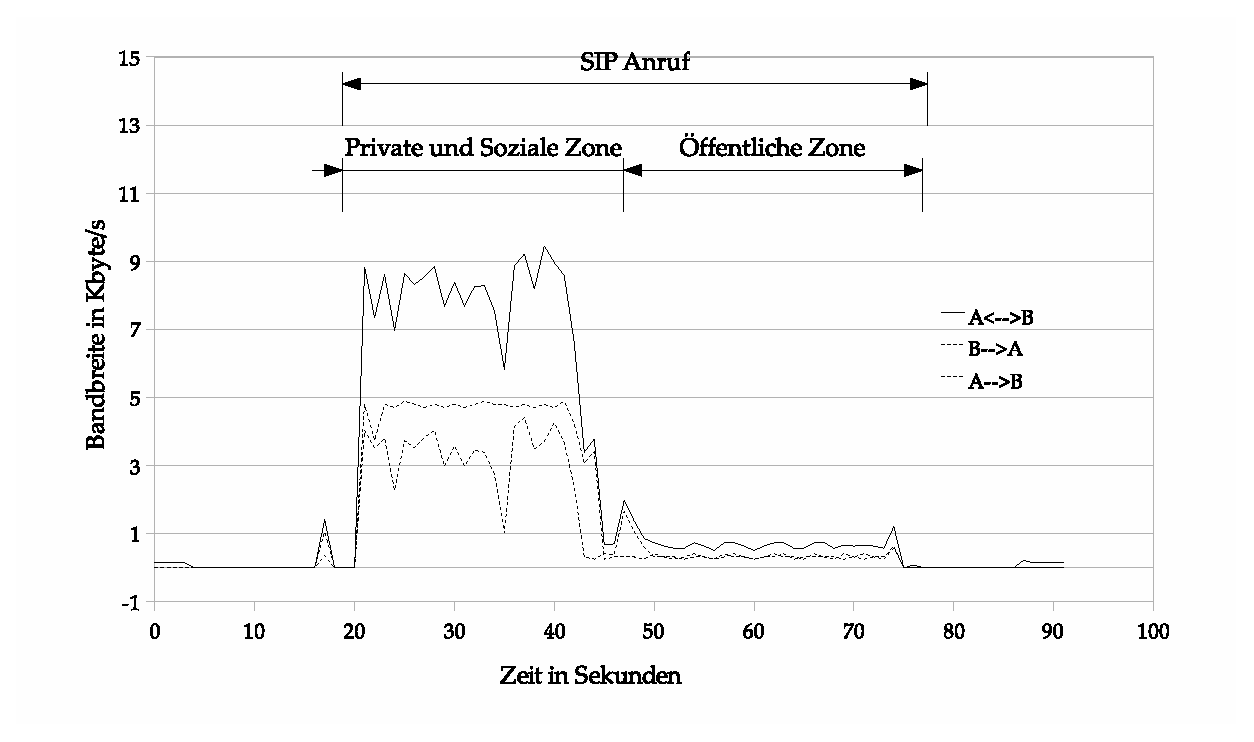
\includegraphics[width=1.00\textwidth]{grafiken/mitvadupdown.eps}
		\caption{Der Up- und Downstream mit der Silcence-Supression-Technik}
	\label{fig:VADupdown}
\end{figure}

\begin{figure}[tbh]
	\centering
		\includegraphics[width=1.00\textwidth]{grafiken/mitvadrtpsip.eps}
		\caption{Der Up- und Downstream mit der Silcence-Supression-Technik}
	\label{fig:VADrtpsip}
\end{figure}

\begin{figure}[tbh]
	\centering
		\includegraphics[width=1.00\textwidth]{grafiken/mitholdupanddown.eps}
		\caption{Der Up- und Downstream mit der SIP-Hold-Technik}
	\label{fig:mitholdupanddown}
\end{figure}

\begin{figure}[tbh]
	\centering
		\includegraphics[width=1.00\textwidth]{grafiken/mithold1.eps}
		\caption{Gegen�berstellung des SIP- und RTP-Traffics mit der SIP-HOLD-Technik}
	\label{fig:mithold1}
\end{figure}


\begin{figure}[tbh]
	\centering
		\includegraphics[width=\textwidth]{grafiken/mitvadund2codecs.eps}
		\caption{Speex mit 16 kHz in der privaten Zone und Speex 8 khZ in der sozialen Zone}
	\label{fig:mitvadund2codecs}
\end{figure}

\begin{figure}[tbh]
	\centering
		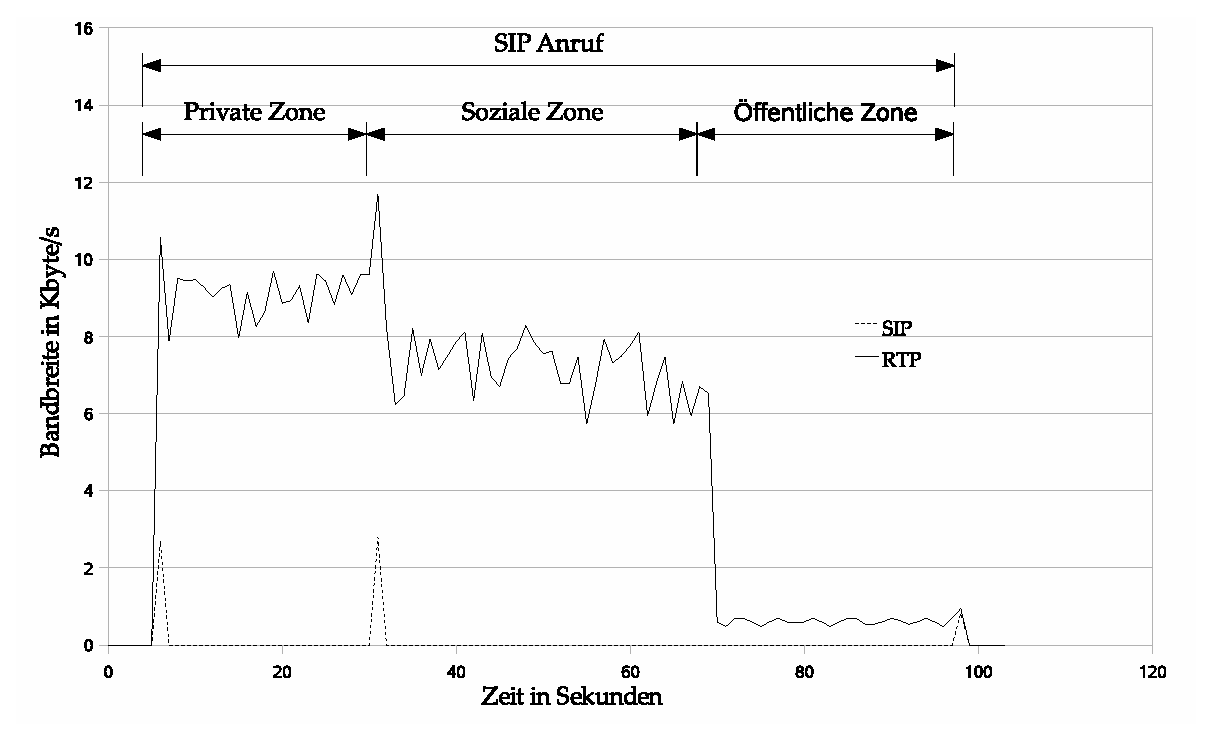
\includegraphics[width=\textwidth]{grafiken/mitvadundrtpsip.eps}
		\caption{Rufauf- und -abbau, sowie Signalisierung eines anderen Codecs mit SIP, Reduktion des Audiostroms mit RTP}
	\label{fig:mitvadundrtpsip}
\end{figure}
%\bibliographystyle{plain}
\bibliographystyle{dinat}
\bibliography{literatur/da}
\chapter*{Eidesstattliche Erkl\"{a}rung}\thispagestyle{empty}Ich versichere, dass ich meine Diplomarbeit ohne Hilfe Dritter und ohne Benutzunganderer als der angegebenen Quellen und Hilfsmittel angefertigt und die den benutzten Quellen w\"{o}rtlich oder inhaltlich entnommenen Stellen als solche kenntlich gemacht habe. Diese Arbeit hat in gleicher oder \"{a}hnlicher Form noch keiner Pr\"{u}fungsbeh\"{o}rde vorgelegen.\bigskip\raggedright{Mannheim, den 17.06.2008} \bigskip \bigskip \bigskip Thomas Plotkowiak
\end{document}